\documentclass[10pt]{article}
\usepackage[a4paper, left=2cm, right=2cm, top=2cm, bottom=2cm]{geometry}
% \usepackage[T1]{fontenc}
% \usepackage{mathptmx}
\usepackage{amsmath,amssymb,amsfonts}
% \usepackage{amsfonts}
% \usepackage{chemformula}
\usepackage{cite}
% \usepackage[colorlinks, linkcolor=black, anchorcolor=black, citecolor=black]{hyperref}
\usepackage{graphicx}
\usepackage[backref]{hyperref}
\usepackage{ntheorem}
\usepackage{float} %设置图片浮动位置的宏包
\usepackage{subfigure} %插入多图时用子图显示的宏包
\usepackage{listings}
\usepackage[framed,numbered,autolinebreaks,useliterate]{mcode}
\usepackage{booktabs}
\usepackage{float}

\newtheorem*{proof}{Proof}[section]

\setlength{\parskip}{0.5em}
\title{Adaptive Signal Processing and Machine Intelligence Coursework}
\author{\textup{Zhaolin Wang}}
\begin{document}

\begin{titlepage}
	\newcommand{\HRule}{\rule{\linewidth}{0.5mm}}
	\includegraphics[width=8cm]{logo_imperial_college_london.png}\\[1cm] 
	\center 
	\quad\\[1.5cm]
	\textsl{\Large Imperial College London }\\[0.5cm] 
	\textsl{\large Department of Electrical and Electronic Engineering}\\[0.5cm] 
	\makeatletter
	\HRule \\[0.4cm]
	{ \huge \bfseries \@title}\\[0.4cm] 
	\HRule \\[1.5cm]
	\Large \@author \\[0.5cm]
	% \begin{minipage}{0.4\textwidth}
	% 	\begin{flushleft} \large
	% 		\emph{Author:}\\
	% 		\@author 
	% 	\end{flushleft}
	% \end{minipage}
	% ~
	% \begin{minipage}{0.4\textwidth}
	% 	\begin{flushright} \large
	% 		\emph{Supervisor:} \\
	% 		\textup{Prof Yang}
	% 	\end{flushright}
	% \end{minipage}\\[3cm]
	\makeatother
	{\large An Assignment submitted for the ICL:}\\[0.5cm]
	{\large \emph{ELEC97003 - Adaptive Signal Processing and Machine Intelligence}}\\[0.5cm]
	{\large \today}\\[2cm] 
	\vfill 
\end{titlepage}

\tableofcontents
\newpage

\section{Classical and Modern Spectrum Estimation}
\subsection{Properties of Power Spectral Density (PSD)}
\ \indent
For a random sequence $x\left[n\right]$, its Power Spectral Density (PSD) 
is defined as
\begin{equation}
	P\left(\omega\right)=\sum_{k=-\infty}^{\infty} {r\left(k\right)e^{-j\omega k}} \label{eq1}
\end{equation}
where $r\left(k\right)$ is the autocorrelation function (ACF) of the sequence $x\left[n\right]$, which is defined as 
\begin{equation}
	r\left(k\right)=\mathbb{E}\left\{x\left[n\right]x^\ast\left[n-k\right]\right\} \label{eq2}
\end{equation}
Apart from definition \eqref{eq1}, the PSD can be defined as
\begin{equation}
	P\left(\omega\right) = \lim_{N\rightarrow\infty}{\mathbb{E}}\left\{\frac{1}{N}\left|\sum_{n=0}^{N-1}{x\left(n\right)e^{-jn\omega}}\right|^2\right\} \label{eq3}
\end{equation}
if the ACF $r\left(k\right)$ decays rapidly, i.e.,
\begin{equation}
	\lim_{N\rightarrow\infty}{\frac{1}{N}}\sum_{k=-\left(N-1\right)}^{N-1}\left|k\right|\left|r\left(k\right)\right|=0 \label{eq4}
\end{equation}
\begin{proof}
	Firstly, the following two vectors are defined                                                                                                                                                                                                                                                                                                                                                                                                                                                                                                                                                                                                                                                                                                                                                                                                                                                                                                                                                                                                                                                                                                                                                                                                                                      
	\begin{gather}
		{\bf{x}}=\left[x\left(0\right),x\left(1\right),\ldots,x\left(N-1\right)\right]^T \label{eq5}\\
		{\bf{e}}=\left[1,e^{-j\omega},\ldots,e^{-j\left(N-1\right)\omega}\right]^T \label{eq6}
	\end{gather}
	The definition \eqref{eq3} can be rewritten as 
	\begin{align}
		P\left(\omega\right) &= \lim_{N\rightarrow\infty}{\mathbb{E}}\left\{\frac{1}{N}\mathbf{e}^H\mathbf{x}\mathbf{x}^H\mathbf{e}\right\} \nonumber \\
		&=\lim_{N\rightarrow\infty} {\frac{1}{N}} {\bf{e}}^H \left[ \begin{matrix} r(0)&r(-1)&\cdots&r(-(N-1)) \\ \cdots&\cdots&\cdots&\cdots \\ r(N-1)&r(N-2)&\cdots&r(0) \end{matrix} \right]{\bf{e}} \nonumber \\
		&=\lim_{N\rightarrow\infty}{\sum_{k=-\left(N-1\right)}^{N-1}{\frac{N-\left|k\right|}{N}r\left(k\right)e^{-j\omega k}}} \nonumber \\
		&=\sum_{k=-\infty}^{\infty}{r\left(k\right)e^{-j\omega k}}-\lim_{N \rightarrow \infty} {\sum_{-\left(N-1\right)}^{N-1}{\left|k\right|r\left(k\right)e^{-j\omega k}}} \label{eq7}
	\end{align}
	If the constrain \eqref{eq4} is satisfied, the second term in \eqref{eq7} becomes zero, 
	and definition \eqref{eq3} is equivalent to \eqref{eq1}. $\hfill\blacksquare$ 
\end{proof}

This equivalence can also be indicated by simulation. Consider the 
following impulse signal and sinusoidal signal:

\begin{subequations}
	\begin{equation}
		x_1(t)=\delta (t) \label{eq8a}
	\end{equation}
	\begin{equation}
		x_2(t)=\sin (2 \pi \times 300t) + 0.2 w(t) \label{eq8b}
	\end{equation}
\end{subequations}
where $w(t)$ is the WGN signal.

Figure \ref{fig1a} shows the ACF and PSD of the impulse signal \eqref{eq8a} calculated by 
definition \eqref{eq3}. As the ACF of the impulse signal decays very fast, 
the PSD defined by \eqref{eq3} is constant, which is the same as the 
theoretical one defined by \eqref{eq1}. While for the sinusoidal signal \eqref{eq8b}, which 
is shown in Figure \ref{fig1b}, the PSD is not the same as the theoretical one 
as the ACF does not decay fast. 

\begin{figure}[htbp]
    \centering
    \subfigure[impulse signal]{
        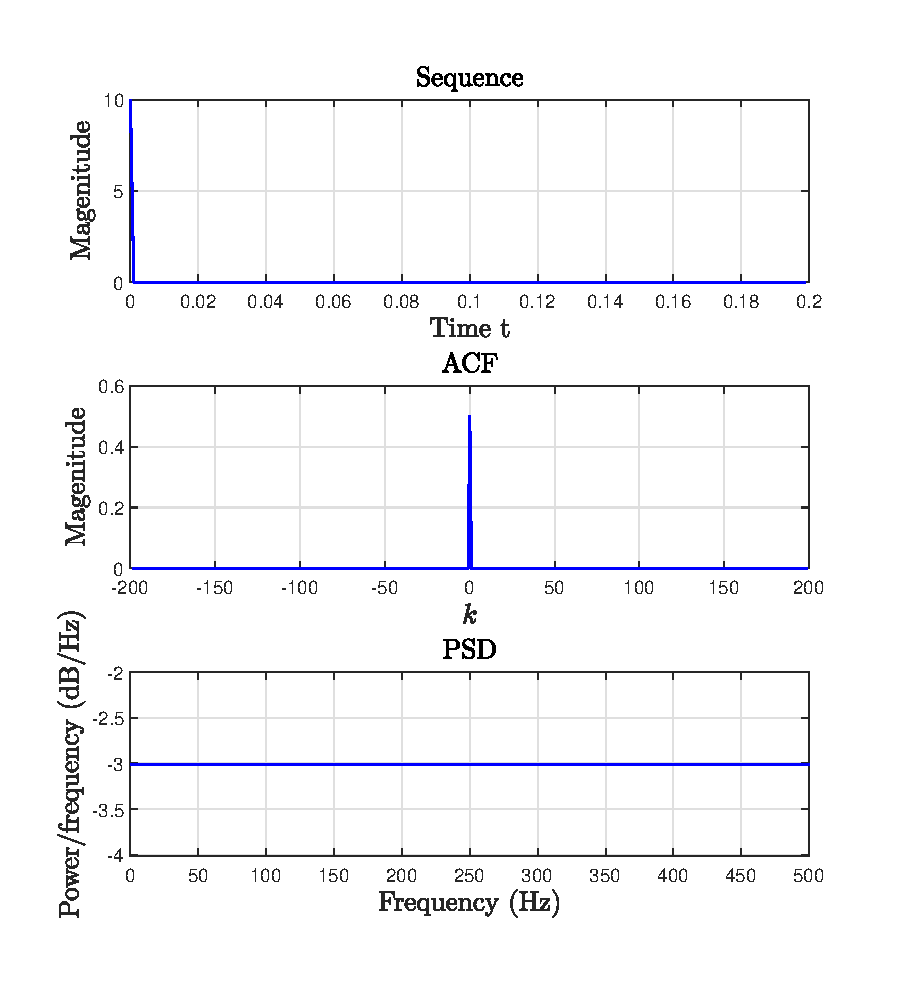
\includegraphics[width=0.48\textwidth]{fig/1.1_1.eps}
        \label{fig1a}
    }
    \subfigure[sinusoidal signal]{
	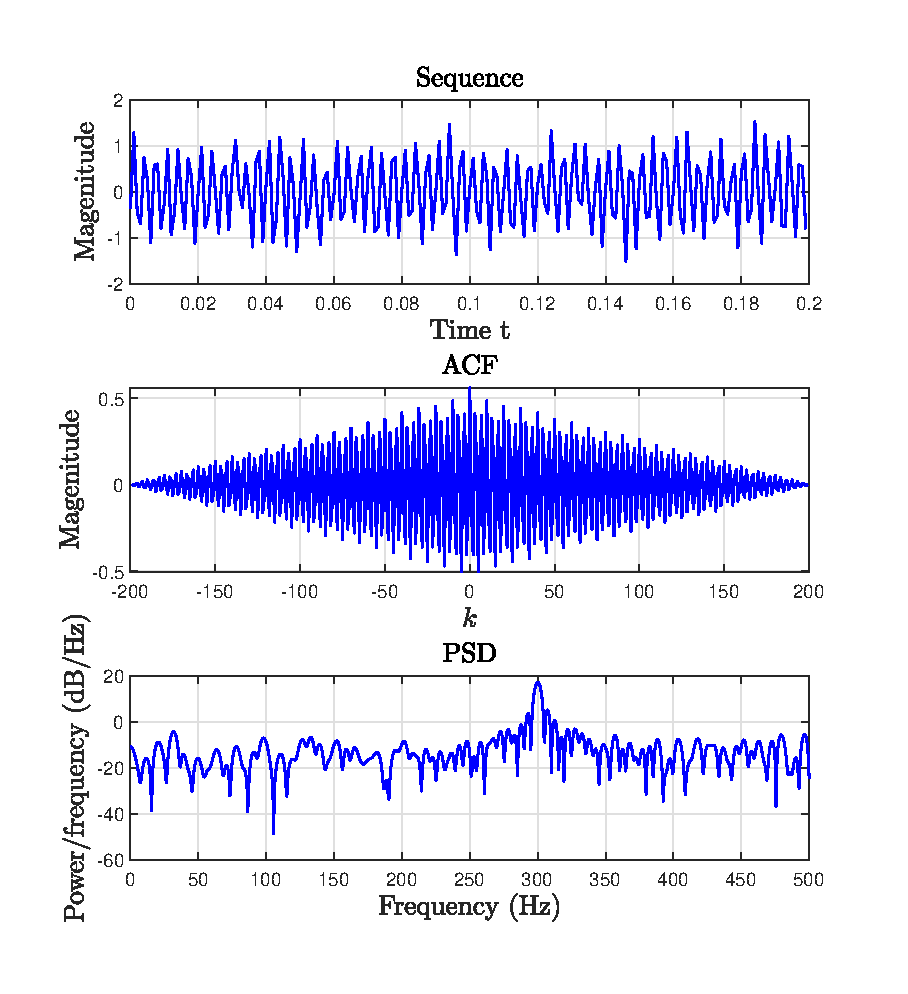
\includegraphics[width=0.48\textwidth]{fig/1.1_2.eps}
        \label{fig1b}
    }
    \caption{ACF and PSD of the signal}
    \label{fig3}
\end{figure}

\subsection{Periodogram-based Methods Applied to Real–World Data}
\ \indent
The Periodogram estimator is defined as 

\begin{equation}
	{\hat{P}}_{per}\left(\omega\right)=\frac{1}{N}\left|\sum_{k=0}^{N-1}{x\left[k\right]e^{-j\omega k}}\right|^2 \label{eq9}
\end{equation}

\subsubsection{Task a: Sunspot Time Series}
\ \indent
Figure \ref{fig2a} shows the comparison of the original and mean-removed sunspot 
data and their PSD. It is noticeable that the value of PSD at 0Hz is 
reduced by about 30dB. The mean value of the sequence contributes to 
the DC component, therefore the DC part (i.e., 0Hz) of the PSD is reduced.

Figure \ref{fig2b} shows the comparison of the original and trend-removed sunspot 
data and their PSD. In contrast to the mean-removed data, the DC component 
of the trend-removed data is almost totally removed (actually the 
magnitude at 0Hz of PSD is lower than -200dB).

Figure \ref{fig2c} shows the comparison of the original and mean-removed logarithmic 
sunspot data. For the latter data, the periodicity is more evident, 
where the magnitude in dB oscillates roughly in the range between -10dB 
and 10dB and its period is around 10 samples.

\begin{figure}[htbp]
    \centering
    \subfigure[Comparison of the original and mean-removed sunspot data (top) and their PSD (bottom)]{
        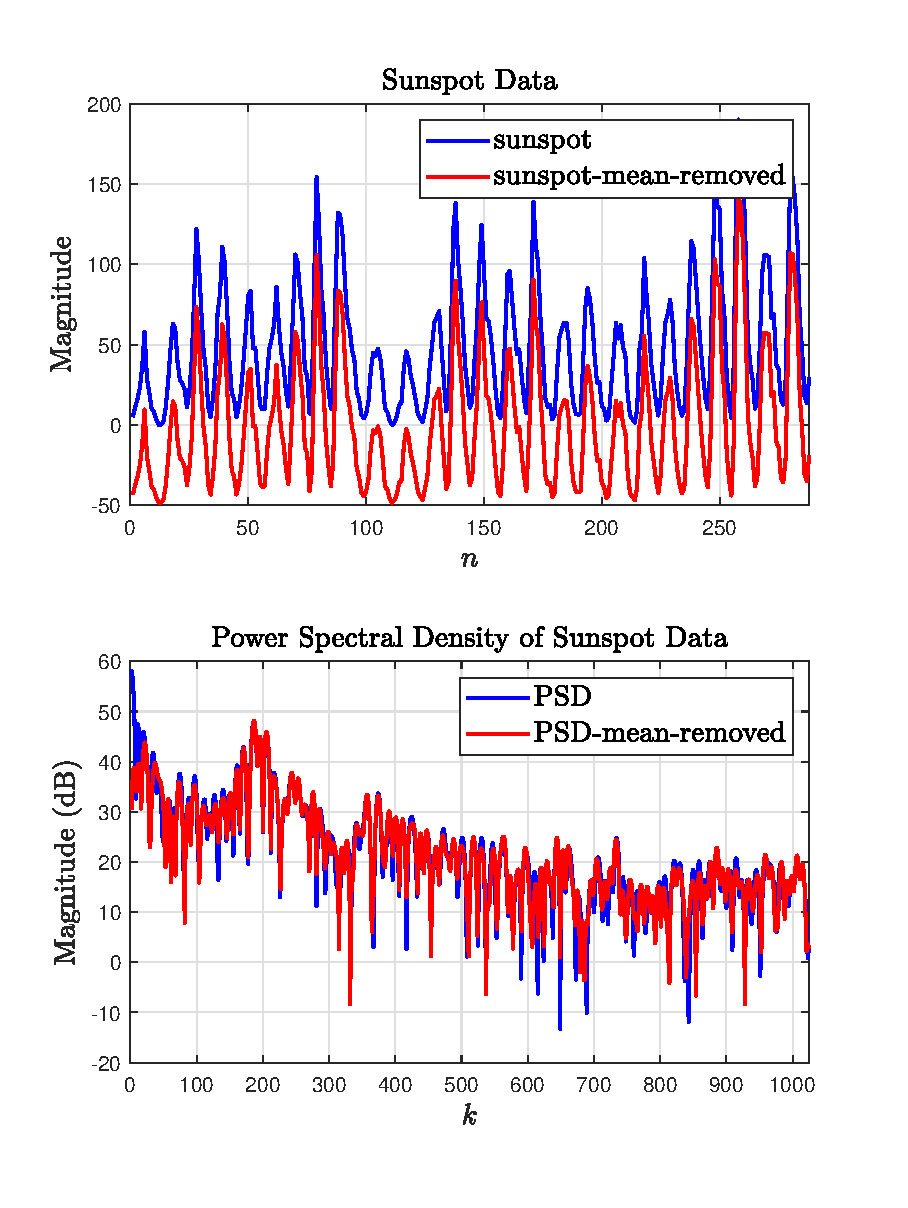
\includegraphics[width=0.31\textwidth]{fig/1.2_1.eps}
        \label{fig2a}
    }
    \subfigure[Comparison of the original and trend-removed sunspot data (top) and their PSD (bottom)]{
		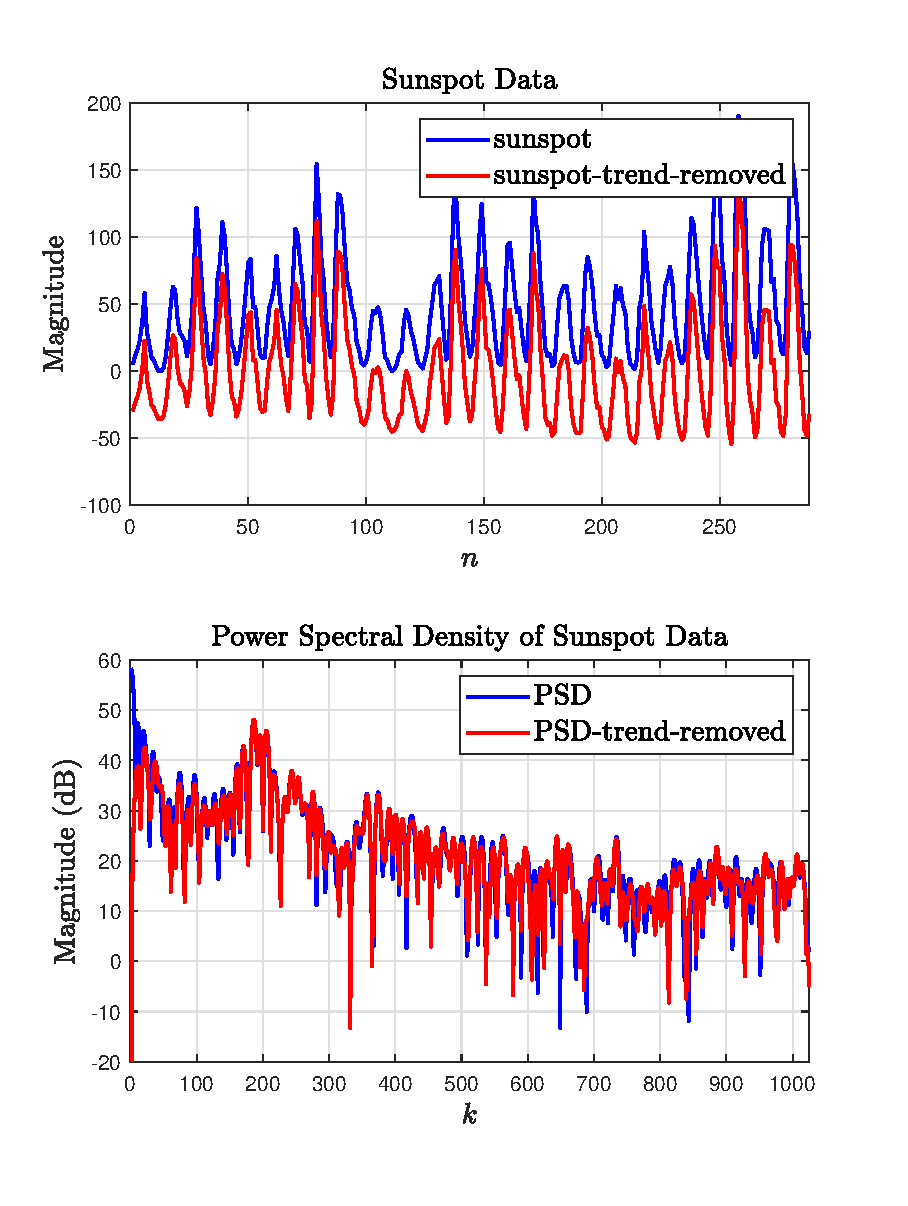
\includegraphics[width=0.31\textwidth]{fig/1.2_2.eps}
        \label{fig2b}
    }
	\subfigure[Comparison of the original (top) and mean-removed logarithmic (bottom) sunspot data.]{
		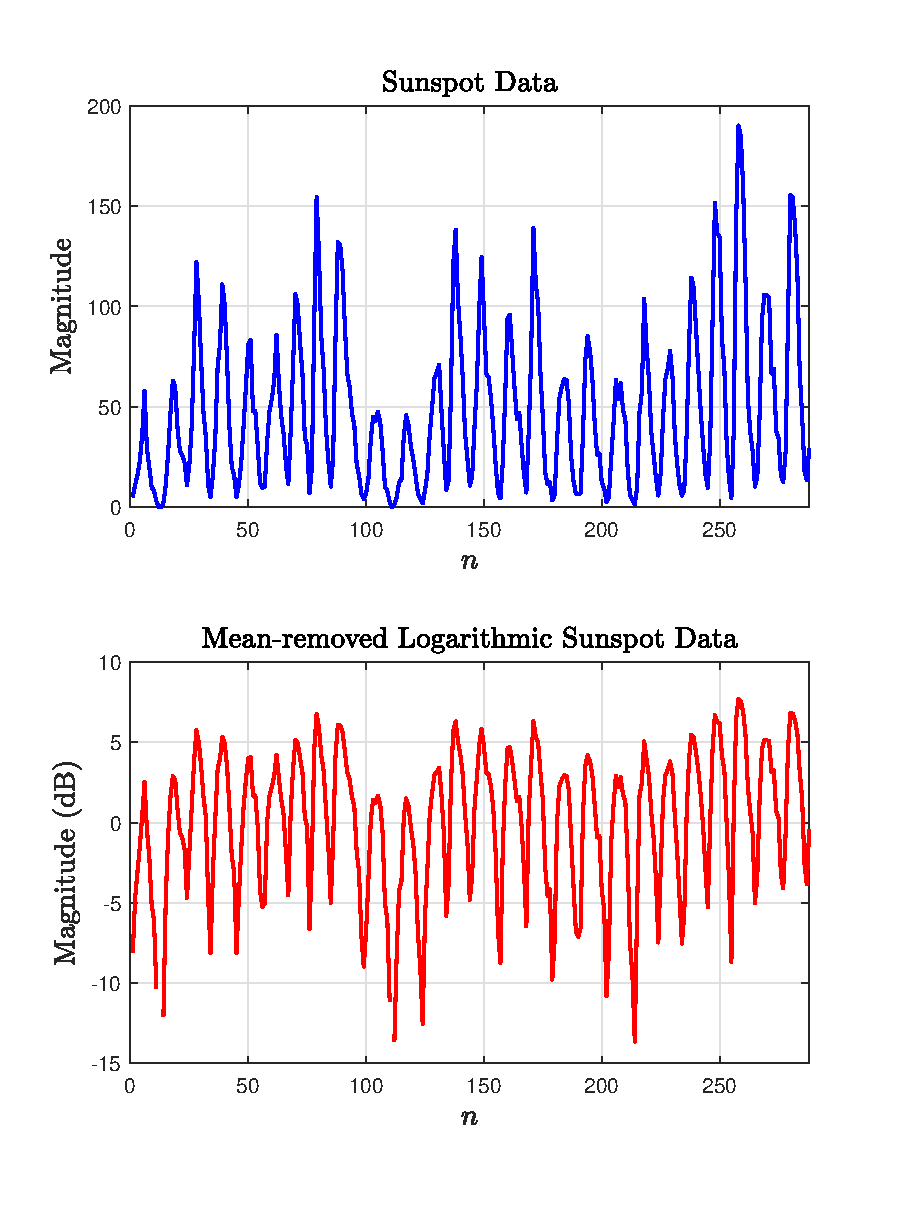
\includegraphics[width=0.31\textwidth]{fig/1.2_3.eps}
		\label{fig2c}
	}
    \caption{Analysis of the sunspot time series data}
    \label{fig2}
\end{figure}

\subsubsection{Task b: EEG Signal}
\ \indent
The Periodogram estimator in \eqref{eq9} is exploited to estimate the PSD of the 
EEG signal. The blue curve in Figure \ref{fig3a} shows the PSD between 11Hz and 20Hz estimated by 
standard Periodogram, which reveals an SSVEP peak at 13Hz.

Bartlett’s method is a modified Periodogram approach, which is averaged 
Periodogram of non-overlapping segments. Three different window lengths 
(10 s, 5 s, and 1 s) are tested. To enable a fair comparison, the 5 DFT 
samples per Hz are kept for all the cases. Figure \ref{fig3a} shows the comparison 
of the standard Periodogram approach and Bartlett’s method with a window 
length of 10s, where the SSVEP peak at 13Hz in the latter method is more 
distinguishable. 

Nevertheless, Bartlett’s method does not always benefit finding the SSVEP 
peaks, as the resolution of PSD is decreased with the decrease of window 
length. Figure \ref{fig3b} shows the effect of window length. In the case where the 
window length is 5s, the PSD result is better than the case where the 
window length is 10s. However, if the window length is very small, 
e.g., 1s in the figure, the peak at 13Hz disappears due to the low 
frequency resolution.

\begin{figure}[htbp]
    \centering
    % \subfigure[PSD estimated by standard periodogram]{
    %     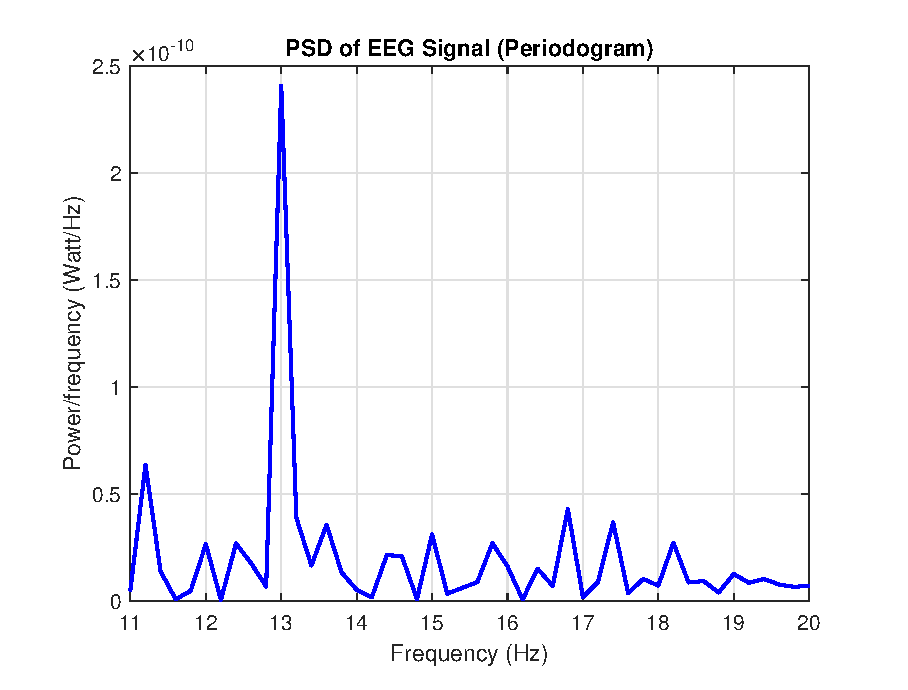
\includegraphics[width=0.31\textwidth]{fig/1.2_4.eps}
    %     \label{fig3a}
    % }
    \subfigure[Comparison of the standard periodogram approach and modified periodogram approach with windows length of 10s]{
		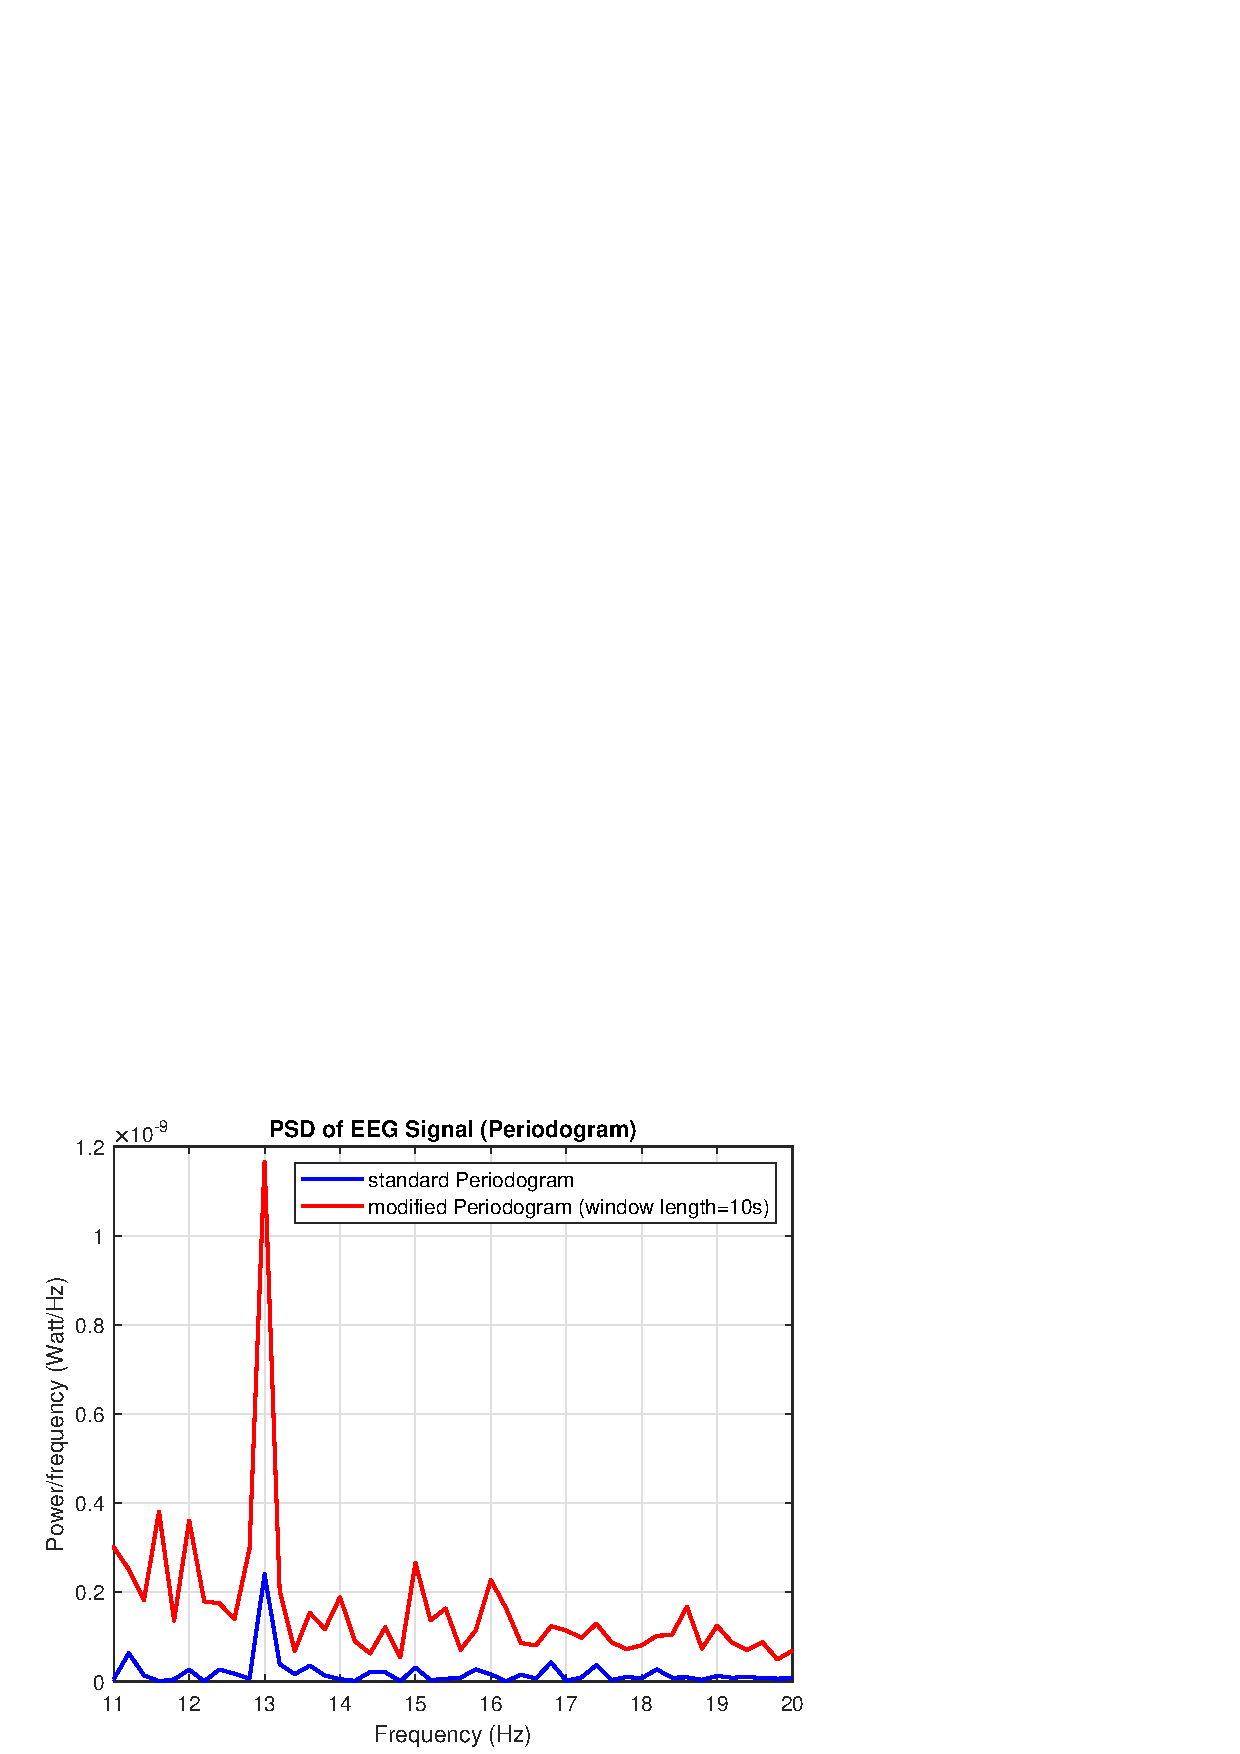
\includegraphics[width=0.47\textwidth]{fig/1.2_5.pdf}
        \label{fig3a}
    }
	\subfigure[Comparison of Bartlett’s method with various window lengths.]{
		\includegraphics[width=0.47\textwidth]{fig/1.2_6.pdf}
		\label{fig3b}
	}
    \caption{Standard Periodogram and Bartlett's Periodogram of the EEG signal}
    \label{fig3}
\end{figure}

\subsection{Correlation Estimation}
\ \indent
Apart from the Periodogram-based method, the Correlogram method can also 
be applied to estimate the PSD, which is defined as 
\begin{equation}
	{\hat{P}}_{corr}\left(\omega\right)=\sum_{k=-\left(N-1\right)}^{N-1}{\hat{r}\left(k\right)e^{j\omega k}} \label{eq10}
\end{equation}
where $\hat{r}\left(k\right)$ is the biased or unbiased estimates of 
autocorrelation function (ACF).

\subsubsection{Task a: Comparison of Biased and Unbiased Estimators}
\ \indent
In order to compare the effect of biased and unbiased estimators of 
ACF in the Correlogram, the following two signals are considered:
\begin{subequations}
	\begin{equation}
		x_3\left(t\right)=0.7\sin{\left(60\pi t\right)}+\sin\left(120\pi t\right)+0.3w\left(t\right) \label{eq11a}
	\end{equation}
	\begin{equation}
		x_4\left(t\right)=w\left(t\right) \label{eq11b}
	\end{equation}
\end{subequations}
where $w\left(t\right) \sim \mathcal{N}(0,1)$ is the WGN signal. 
These two signals are sampled with the sampling frequency $f_s=200$Hz 
and $N=128$ samples are obtained. For the second pure WGN signal, the 
averaged ACF and Correlogram PSD of 1000 realizations are calculated.

Figure \ref{fig4a} shows the ACF the PSD of biased and unbiased estimates of the 
noisy sinusoidal signal \eqref{eq11a}. For the unbiased estimate of ACF, it is 
noticeable that the value is larger than that of the biased estimate for 
large lags. However, the unbiased estimate is subjected to high uncertainty for large 
lags, due to the fewer available samples.

On the other hand, the biased estimate applies low weights for the large 
lags, which reduces the uncertainty and makes the biased estimate more 
reliable. This can be indicated by the more oscillation in the PSD 
estimated by unbiased ACF, whose variance is higher. 
Furthermore, the unbiased ACF may result in the negative values of 
estimated PSD.

Figure \ref{fig4b} shows the average ACF of PSD of biased and unbiased estimates 
of 1000 realizations of the pure WGN signal \eqref{eq11b}. Both PSD 
functions estimated by the biased and unbiased ACF oscillate around the 
theoretical PSD (i.e., $P\left(\omega\right)=1$). However, 
the oscillation range of the unbiased estimate is higher than the 
biased one, which indicates the higher variance of the unbiased 
estimate again.

\begin{figure}[htbp]
    \centering
    \subfigure[ACF (top) and Correlogram PSD (bottom) of sampled signal \eqref{eq11a}]{
        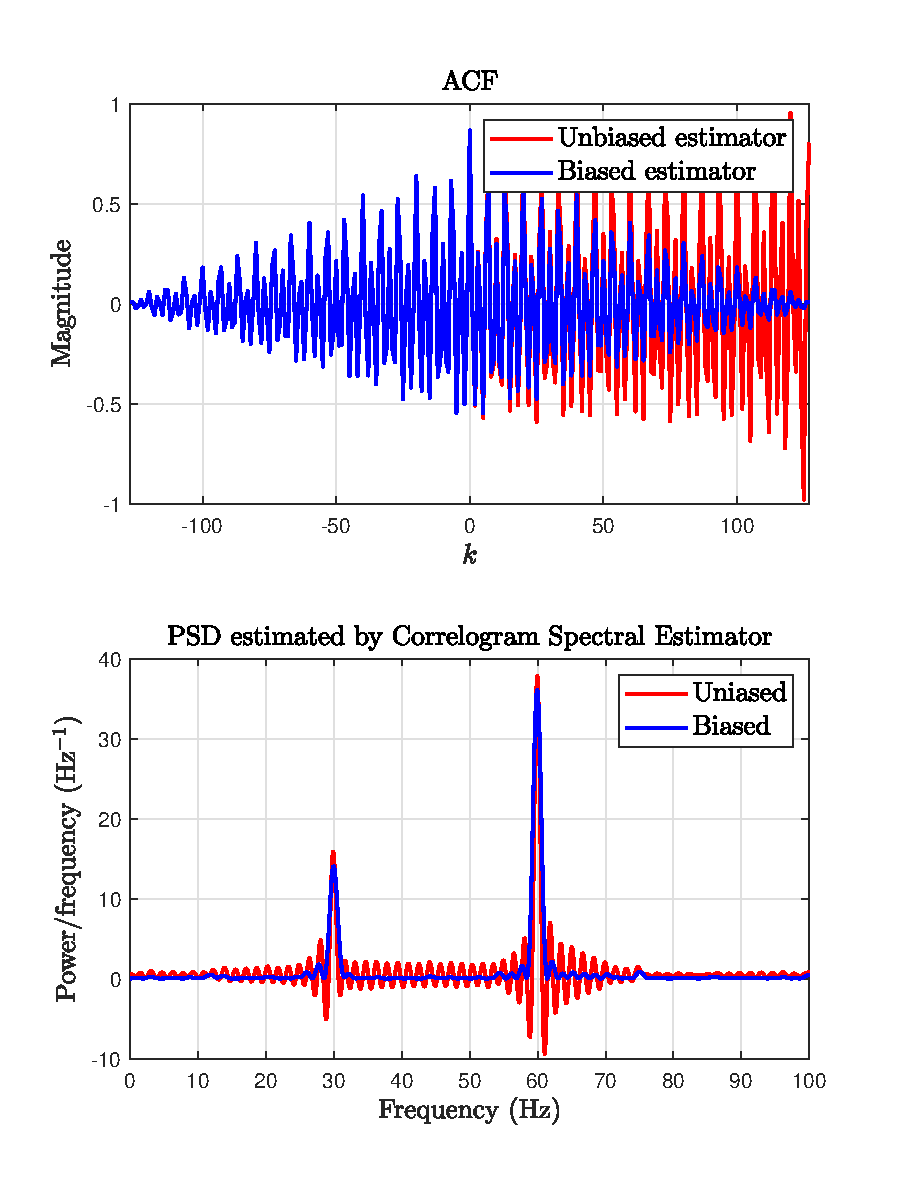
\includegraphics[width=0.48\textwidth]{fig/1.3_1.eps}
        \label{fig4a}
    }
    \subfigure[ACF (top) and Correlogram PSD (bottom) of sampled signal \eqref{eq11b}]{
	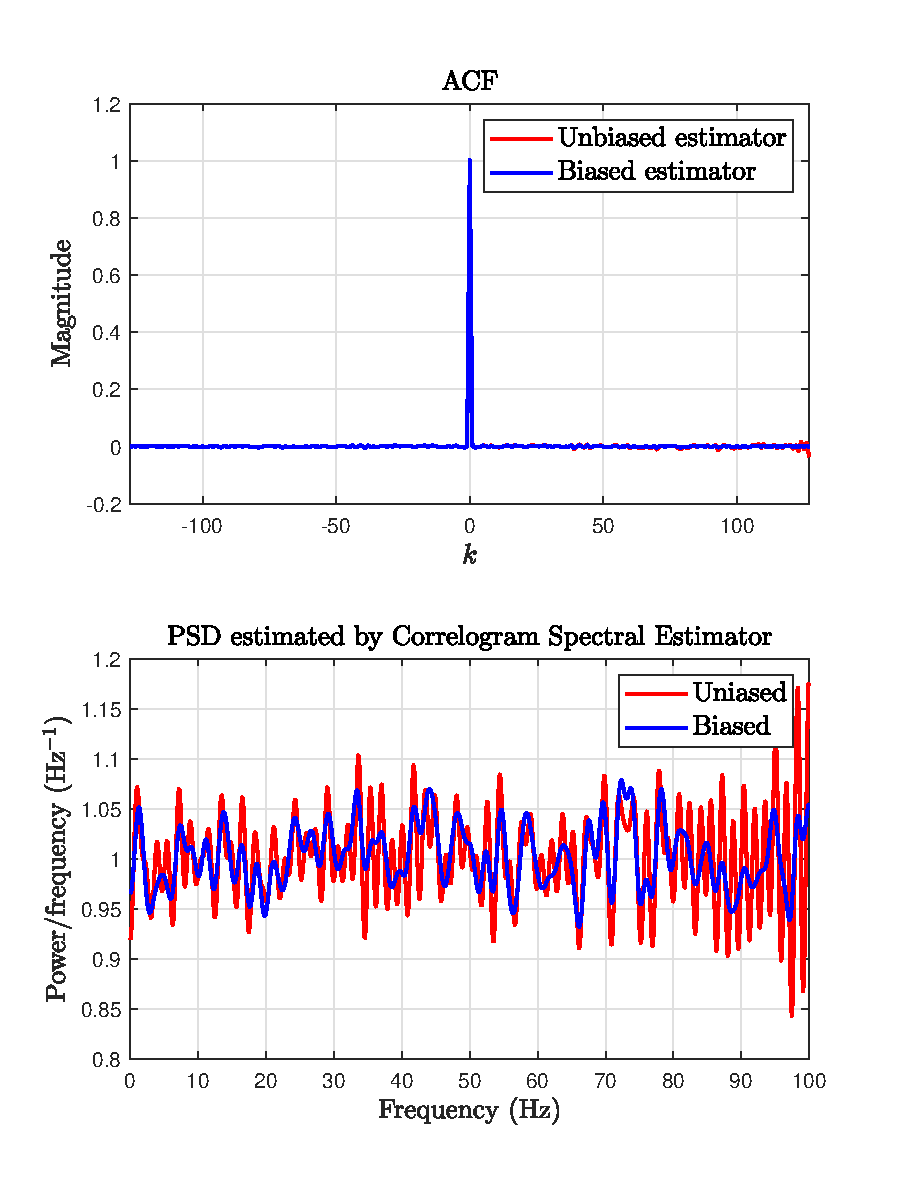
\includegraphics[width=0.48\textwidth]{fig/1.3_2.eps}
        \label{fig4b}
    }
    \caption{Comparsion of biased and unbiased estimator}
    \label{fig4}
\end{figure}

\subsubsection{Task b \& c: Plotting in dB}
\ \indent
The effect of plotting PSD in dB is investigated in this part. The biased 
ACF estimator of noisy sinusoidal signal \eqref{eq11a} is considered. In Figure \ref{fig5a}, 
the PSD estimates of 100 realizations and their mean are not plotted in dB. 
We can see that the different realizations of the spectral estimate are 
more disperse at the frequency near 30Hz and 60Hz, where the values of 
PSD are high. This phenomenon can also be indicated by the higher value 
of the standard deviation near 30Hz and 60Hz. However, the high-value part 
of PSD is usually what we are interested in.

\begin{figure}[htbp]
    \centering
    \subfigure[PSD estimates of signal \eqref{eq11a}. Top: an overlay of 100 realizations and their mean. Bottom: standard deviation of the 100 realizations.]{
        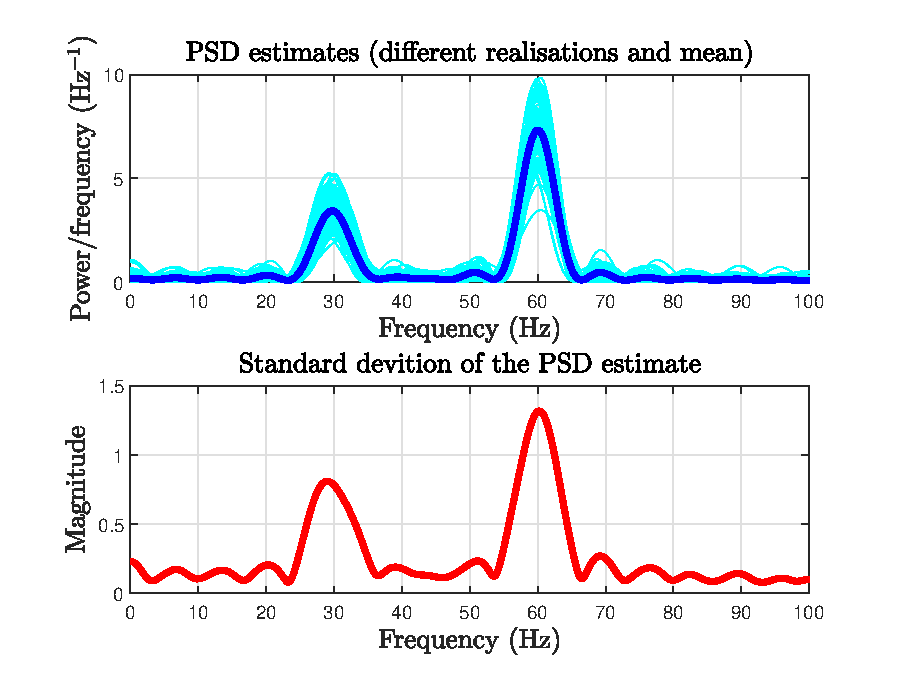
\includegraphics[width=0.48\textwidth]{fig/1.3_3.eps}
        \label{fig5a}
    }
    \subfigure[PSD estimates of signal \eqref{eq11a} plotted in dB. Top: an overlay of 100 realizations and their mean. Bottom: standard deviation of the 100 realizations.]{
	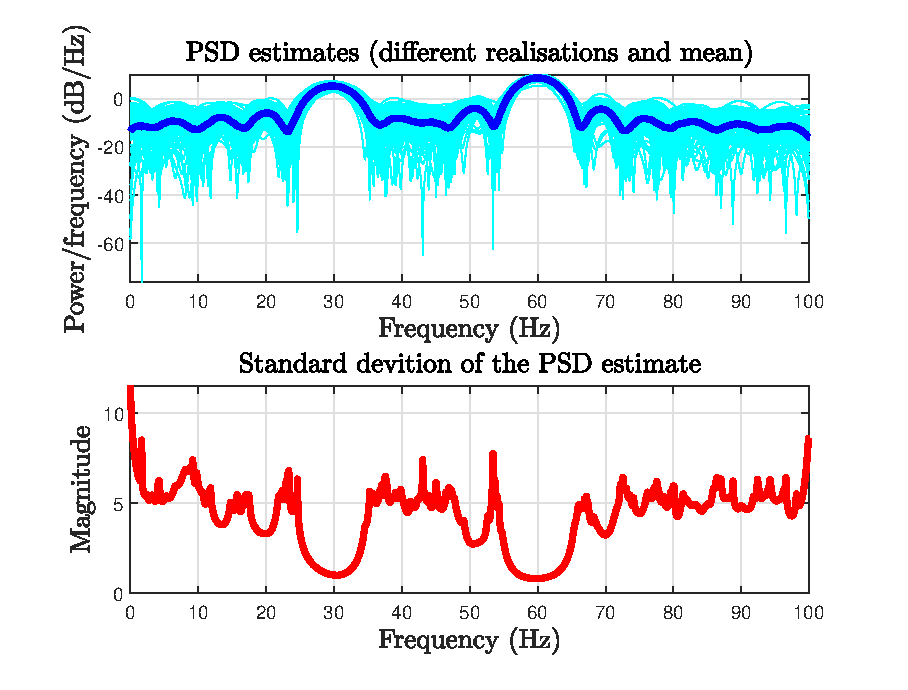
\includegraphics[width=0.48\textwidth]{fig/1.3_4.eps}
        \label{fig5b}
    }
    \caption{Comparison of standard plot and "dB" plot}
    \label{fig5}
\end{figure}

Figure \ref{fig5b} plots the PSD estimates in dB and then the average PSD 
is calculated. In this case, the estimates of PSD are less spread out at 
the high value of PSD and the standard deviation is inversely proportional 
to the value of PSD. Therefore, there is less uncertainty at the positions 
that we are interested in the PSD.

\subsubsection{Task d \& e: Frequency Estimation by MUSIC}
\ \indent
For the classic Periodogram approach, the frequency 
resolution of estimated PSD is limited by the length $N$ of sequence, 
and the resolution is proportional to $1/N$. 

\begin{figure}[htbp]
    \centering
    \subfigure{
        \includegraphics[width=0.48\textwidth]{fig/1.3_5_1.pdf}
    }
    \subfigure{
		\includegraphics[width=0.48\textwidth]{fig/1.3_5_2.pdf}
    }
	\subfigure{
        \includegraphics[width=0.48\textwidth]{fig/1.3_5_3.pdf}
    }
    \subfigure{
		\includegraphics[width=0.48\textwidth]{fig/1.3_5_4.pdf}
    }
    \caption{Periodogram of the complex exponential with different length}
    \label{fig6}
\end{figure}

Figure \ref{fig6} shows the Periodogram estimates of the following signal:
\begin{equation}
	x_5\left(t\right)=e^{j2\pi\times0.3t}+e^{j2\pi\times0.32t}+0.2n\left(t\right) \label{eq12}
\end{equation} 
where $n\left(t\right) \sim \mathcal{CN}(0,1)$ is the complex Gaussian noise.

% \begin{figure}[htbp]
% 	\centering
% 	\includegraphics[width=1\textwidth]{fig/1.3_5.eps}
% 	\caption{Periodogram of the complex exponential with different length}
% 	\label{fig6}
% \end{figure}

This signal is sample with $f_s=1$Hz. In Figure \ref{fig6}, the two frequency 
components 0.3Hz and 0.32Hz cannot be distinguished when the length of 
sampled sequence is 30, due to the low frequency resolution. With 
the increase of the sequence length, the two frequency components start to 
be distinguishable and the Periodogram spectrum starts showing the correct line 
spectra of the signal \eqref{eq12}, which has high main-lobe level at frequency 
0.3Hz and 0.32Hz and low side-lobe level at other frequencies.

The MUSIC is a subspace method for spectral estimation, which is defined as
\begin{equation}
	{\hat{P}}_{\text{MUSIC}}\left(\omega\right)=\frac{1}{\sum_{i=p+1}^{M}\left|\mathbf{e}^H\mathbf{v}_i\right|^2} \label{eq13}
\end{equation}
where $M$ is the length of the signal sequence, $p$ is the number of 
frequency components in the signal, $\mathbf{e}=\left[1,e^{j\omega},\ldots,e^{j\omega\left(M-1\right)}\right]$ is the 
basis vector, and $\mathbf{v}_i$ is the eigenvector corresponding to the 
$i$-th eigenvalue ranking from the largest to the smallest. If $\omega_1$ is 
one of the frequency components in the signal and $\mathbf{e}_1$ is the 
corresponding basis vector, we have
\begin{equation}
	\mathbf{e}_1^H\mathbf{v}_i=0 \label{eq14}
\end{equation}
Therefore, ${\hat{P}}_{\text{MUISC}}\left(\omega\right)$ will have a 
large value at the frequency component $\omega_1$.

In this part, the following code is applied to find the desired line 
spectra of signal \eqref{eq12}, which is sample at $f_s=1$Hz and has a 
length of $N=30$, using the MUSIC method. 

\begin{lstlisting}
	[X,R] = corrmtx(x,14,'mod');
	[S,F] = pmusic(R,2,[ ],1,'corr');
	plot(F,S,'linewidth',2); set(gca,'xlim',[0.25 0.40]);
	grid on; xlabel('Hz'); ylabel('Pseudospectrum');
\end{lstlisting}

The first line in the code is to estimate the covariance matrix of 
the sequence. The first input argument for the function $\mathtt{corrmtx}$ 
is the signal sequence $x\left[n\right]$. Let the second argument is 
denoted by $M$, then the first output of $\mathtt{corrmtx}$ with the $\mathtt{'mod'}$ 
argument is a $2\left(N-M\right)\times\left(M+1\right)$ matrix, 
which is defined as 
\begin{equation}
	\mathbf{H}=\frac{1}{\sqrt{2(N-M)}} \left[\begin{matrix}
		x(M+1) & \cdots & x(1)\\
		\vdots & \ddots & \vdots\\
		x(N) & \cdots & x(N-M)\\
		x^*(1) & \cdots & x^*(M+1)\\
		\vdots & \ddots & \vdots\\
		x^*(N-M) &\cdots & x^*(M)
	\end{matrix} \right] \label{eq15}
\end{equation}

and the second output of $\mathtt{corrmtx}$ is the covariance matrix, which is defined as
\begin{equation}
	\mathbf{R}=\mathbf{H}^H\mathbf{H} \label{eq16}
\end{equation}
According to \eqref{eq16} $\mathbf{R}$ is an $\left(M+1\right)\times\left(M+1\right)$
matrix, each entry of which is calculated by averaging $2\left(N-M\right)$ 
samples to get the expected value. 

The second line of the code is to calculate the line spectra defined 
in \eqref{eq13}. The first argument of $\mathtt{pmusic}$ is the covariance matrix calculated 
by \eqref{eq16}, the second argument is the number of frequency components $p$, 
the forth argument is the sampling frequency, and the last one is to 
indicate that the first argument should be the covariance matrix. For 
the outputs of $\mathtt{pmusic}$, the first one is the estimated line 
spectra and the second one is the corresponding frequency interval. 

\begin{figure}[htbp]
	\centering
	\includegraphics[width=0.48\textwidth]{fig/1.3_6.pdf}
	\caption{Spectrum estimated by MUSIC.}
	\label{fig7}
\end{figure}

Figure \ref{fig7} shows the spectrum of \eqref{eq12} estimated by MUSIC, 
where the two frequency components at 0.3Hz and 0.32Hz can be 
clearly identified although the length of sequence is only $N=30$. 
Therefore, the MUSIC method can still have good performance to identify
the frequency components with small sequence length, which outperforms 
the Periodogram method. Nevertheless, the number of frequency components 
need to be known for the MUSIC, as it is based on the orthogonality of 
the frequency basis vector and the noise space vector (equation \eqref{eq14}). 

Furthermore, the MUSIC method can be evaluated for any frequency, 
while for the Periodogram can only evaluate the frequency of the 
DFT bins. In this case, the MUSIC method has higher accuracy of the 
estimated spectrum.

\subsection{Spectrum of Autoregressive Processes}
\ \indent
The model of an AR process is given as
\begin{equation}
	x[n] = \sum_{k=1}^p a_k x[n-k] \label{eq17}
\end{equation}
For AR process, its power spectrum is given by
\begin{equation}
	P_{\text{AR}}\left(\omega\right)=\frac{\sigma_w^2}{\left|1-\sum_{k=1}^{p}{a_ke^{-jk\omega}}\right|^2} \label{eq18}
\end{equation}
where $\sigma_w^2$ is the noise power, $p$ is the order of AR process, 
and $a_k$ are the AR coefficients. The $\sigma_w^2$ and $a_k$ can be estimated 
using the Yule-Walker equations with biased ACF estimates or unbiased ACF 
estimates.

\begin{figure}[htbp]
    \centering
    \subfigure[Estimated PSD of AR process using different orders with 1$0^3$ samples.]{
        \includegraphics[width=0.48\textwidth]{fig/1.4_1.eps}
        \label{fig8a}
    }
    \subfigure[Estimated PSD of AR process using different orders with $10^4$ samples.]{
		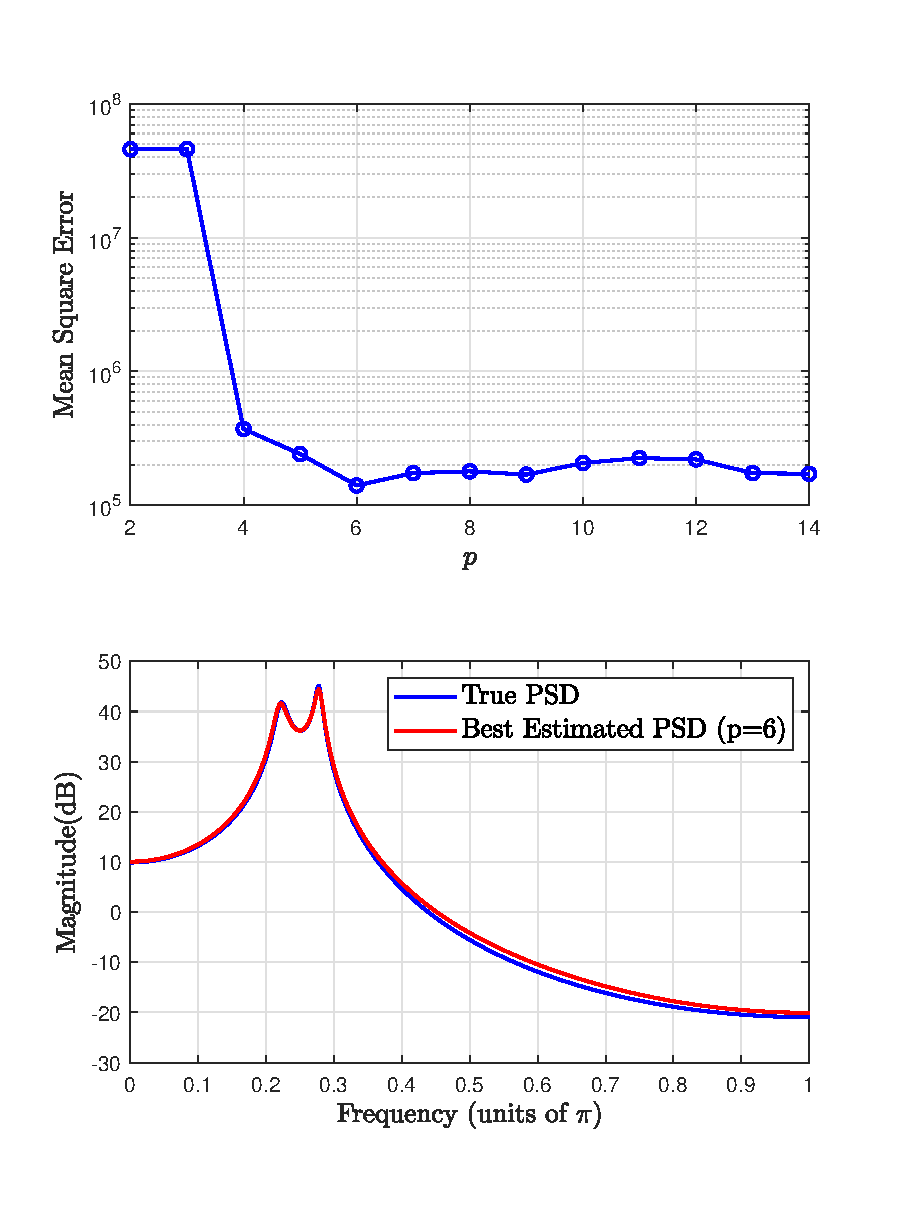
\includegraphics[width=0.48\textwidth]{fig/1.4_2.eps}
        \label{fig8b}
    }
    \caption{Estimated PSD of AR process}
    \label{fig8}
\end{figure}

\subsubsection{Task a: Shortcomings of Unbiased ACF}
\ \indent
In the Yule-Walker equations, if the biased ACF estimate is applied, 
there can be high erratic for the large lags, which may lead to the high 
uncertainty of the estimated AR coefficients. Therefore, the biased 
estimate of the ACF is a better choice.

\subsubsection{Task b \& c: AR Spectrum Estimation}
\ \indent
In this part, the following AR coefficient is considered
\begin{equation}
	{\bf{a}} = [2.76,-3.81, 2.65,-0.92]^T \label{eq19}
\end{equation}
and the noise power is assumed to be $\sigma_w^2=1$.

Figure \ref{fig8a} shows the true PSD of the AR process and the best-estimated 
PSD ($p=12$) using $10^3$ samples, as well as the error of the estimated at 
each order. This figure indicates that by increasing the order of the 
assumed model, the error is generally reduced.

Figure \ref{fig8b} shows the results of $10^4$ samples. It is noticeable that when 
the model order is lower (under-modeling) than the true order, i.e., $p=4$, 
the error is dramatically decrease as the model order increase, while for 
the higher order (over-modeling), although the error generally decreases, 
the reduction of error is not obvious with the increase of model order.

\subsection{Real World Signals: Respiratory Sinus Arrhythmia from RR-Intervals}
\ \indent
In order to better observe the frequencies of respiration in the spectrum, 
the trend of the RRI data in the three trails is firstly removed using 
$\mathtt{detrend}$ to remove the DC component.

\begin{figure}[htbp]
    \centering
    \subfigure[Standard Periodogram spectrum estimates for the RRI data in the three trials.]{
        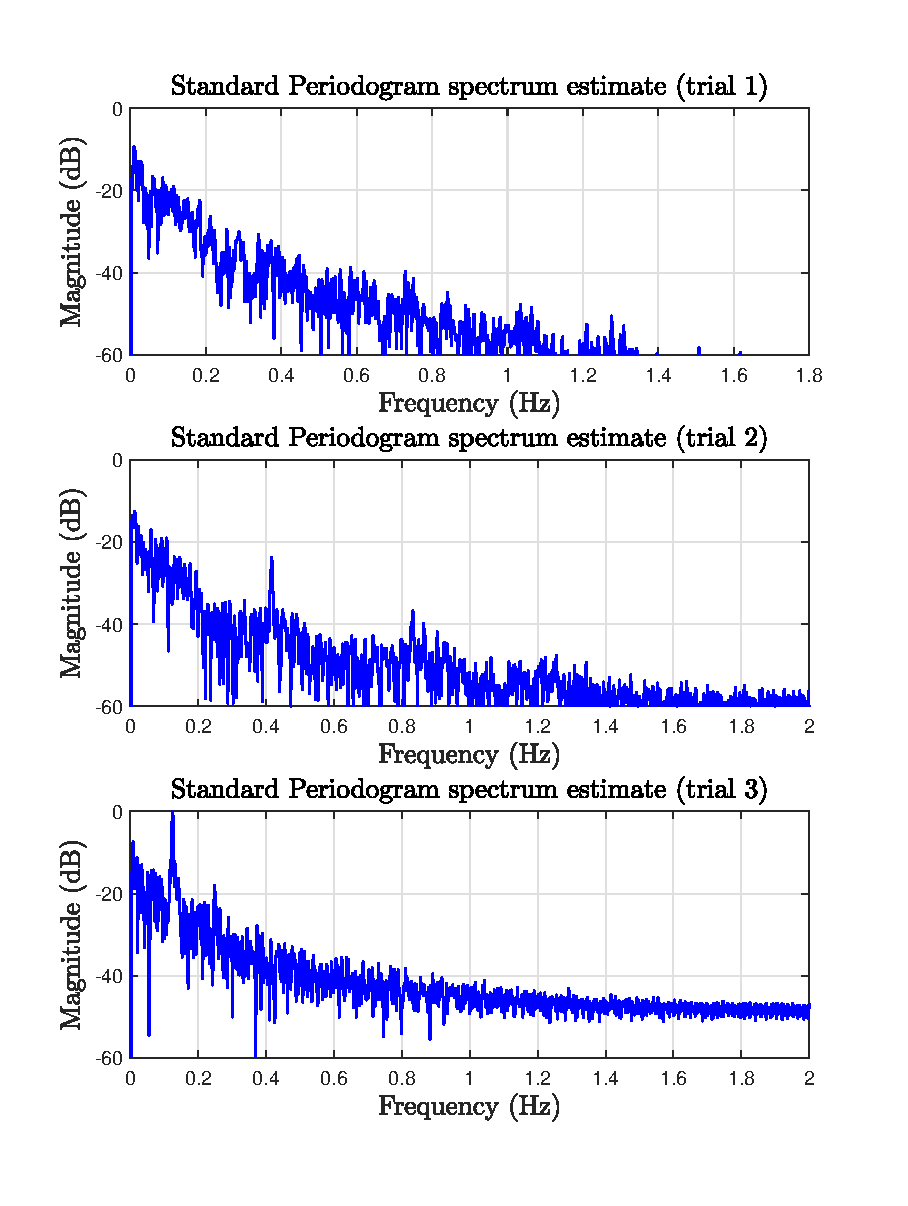
\includegraphics[width=0.48\textwidth]{fig/1.5_1.eps}
        \label{fig9a}
    }
    \subfigure[Averaged Periodogram spectrum estimates for the RRI data in the three trials.(windows length is 50s).]{
		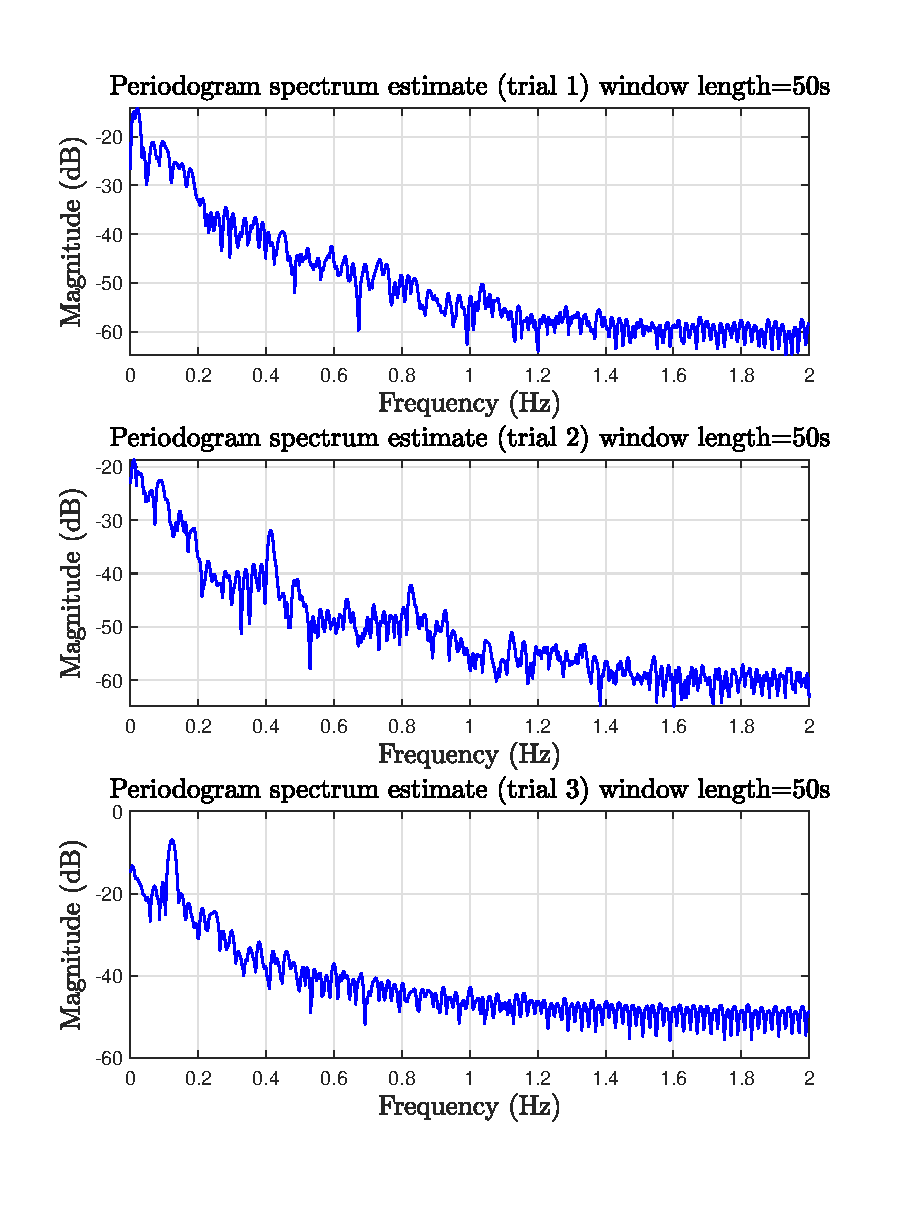
\includegraphics[width=0.48\textwidth]{fig/1.5_2.eps}
        \label{fig9b}
    }
	\subfigure[Averaged Periodogram spectrum estimates for the RRI data in the three trials.(windows length is 150s).]{
		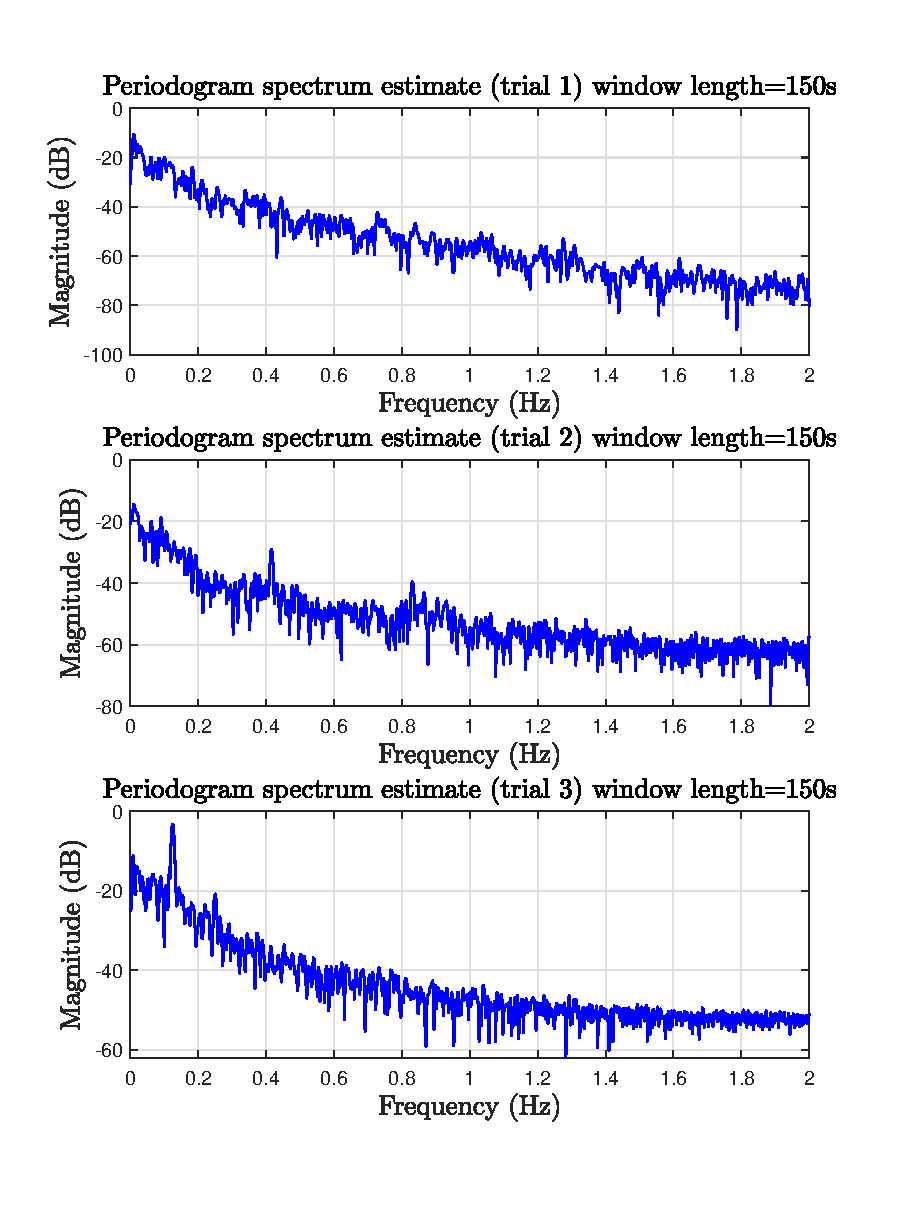
\includegraphics[width=0.48\textwidth]{fig/1.5_4.eps}
        \label{fig9c}
    }
	\subfigure[AR spectrum estimates for the RRI data in the three trials. (AR model order is 40).]{
		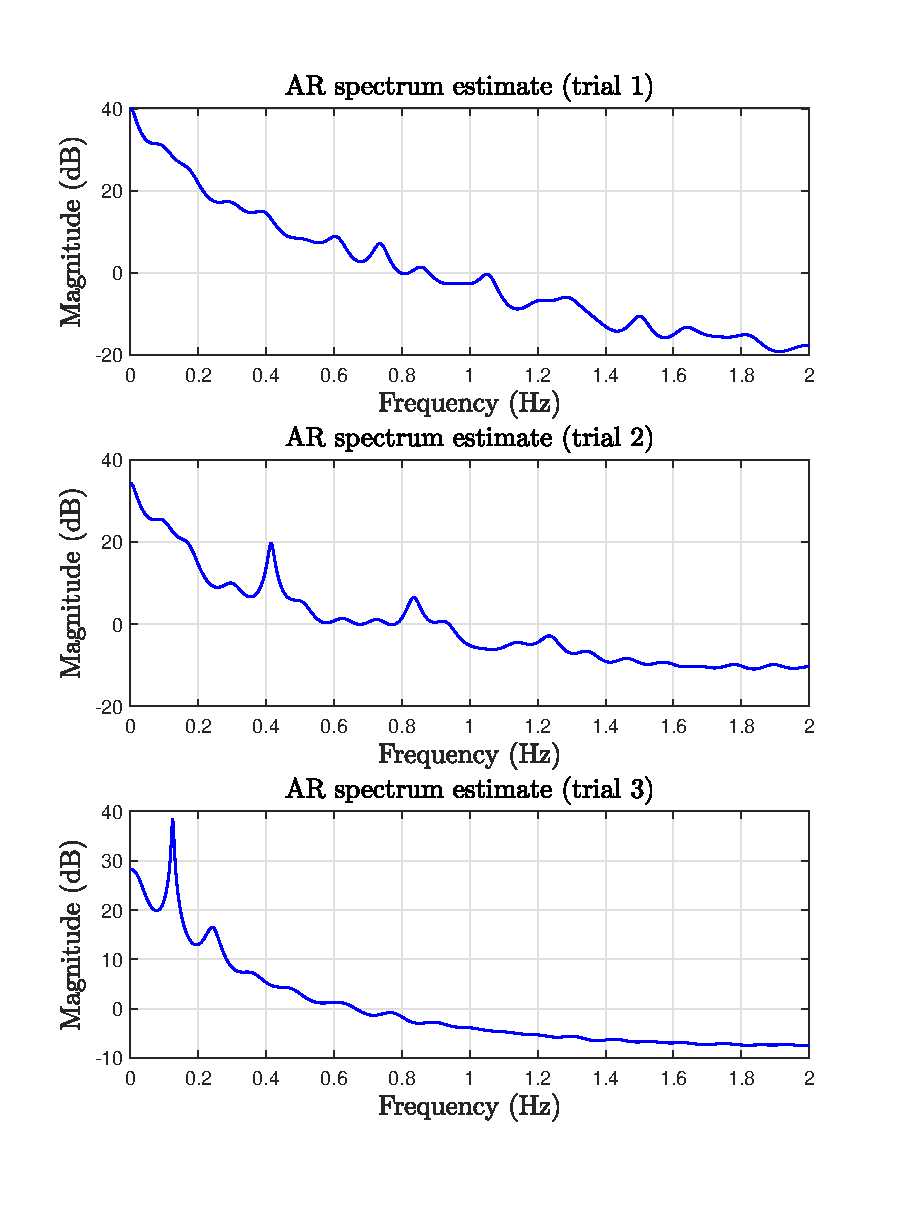
\includegraphics[width=0.48\textwidth]{fig/1.5_3.eps}
        \label{fig9d}
    }
    \caption{Periodogram and AR spectrum estimates for the RRI data}
    \label{fig9}
\end{figure}

\subsubsection{Task a \& b: Periodogram Estimates of PSD}
\ \indent
Figure \ref{fig9a} shows the standard Periodogram spectrum estimates for the RRI 
data in the three trials. Figure \ref{fig9b} and Figure \ref{fig9c} shows the average 
Periodogram spectrum with window lengths of 50s and 150s, respectively.

The main difference between the PSD estimates for the trails is that 
there are no obvious peaks in the PSD for the first trail while both 
the others have the obvious peaks. In the PSD for the second trial, 
the peak appears at the frequency of 0.4Hz, which matches the 25 breaths 
per minute in the trail. In the third trial, the peak is at around 0.12Hz, 
which matches the 7.5 breaths per minute in this trial.

\subsubsection{Task c: AR Spectrum Estimates}
\ \indent
Figure \ref{fig9d} shows the AR spectrum estimates for the RRI in the three trails, 
where the order of the AR model is 40. We can see that the AR spectrum 
estimates is also capable of revealing the frequency peaks. Compared 
with the Periodogram estimates, there are two main difference:
\begin{itemize}
	\item The spectrum power density at each frequency in the two kinds 
	of spectrum estimates are different.
	\item The AR spectrum estimate is capable of showing the frequency 
	components clearer than the Periodogram estimate.
\end{itemize}

% \begin{figure}[htbp]
% 	\centering
% 	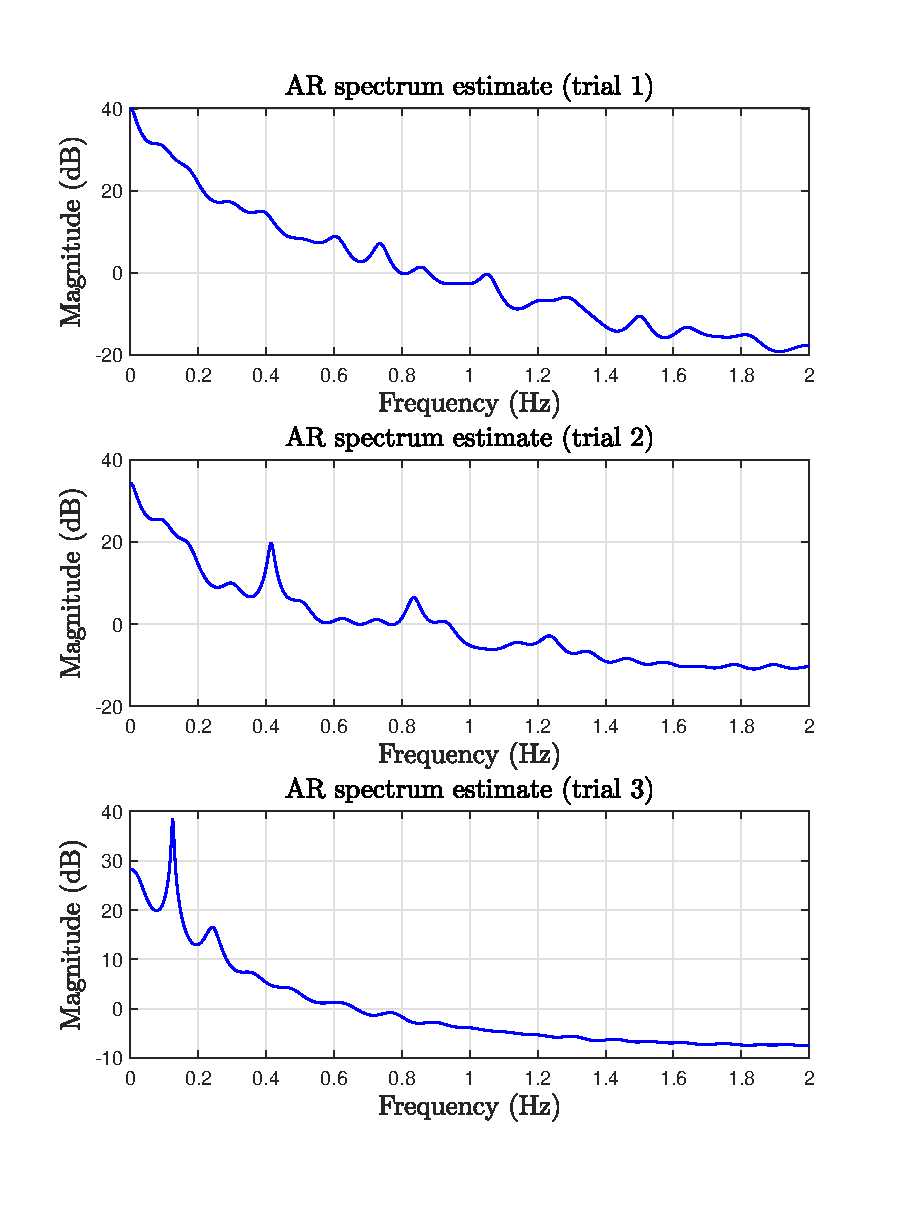
\includegraphics[width=0.45\textwidth]{fig/1.5_3.eps}
% 	\caption{AR spectrum estimates for the RRI data in the three trials. (AR model order is 40).}
% 	\label{fig10}
% \end{figure}

\begin{figure}[htbp]
    \centering
	\subfigure[Singular values of the $\bf{X}$ and ${\bf{X}}_{noise}$ and the square errors between them.]{
		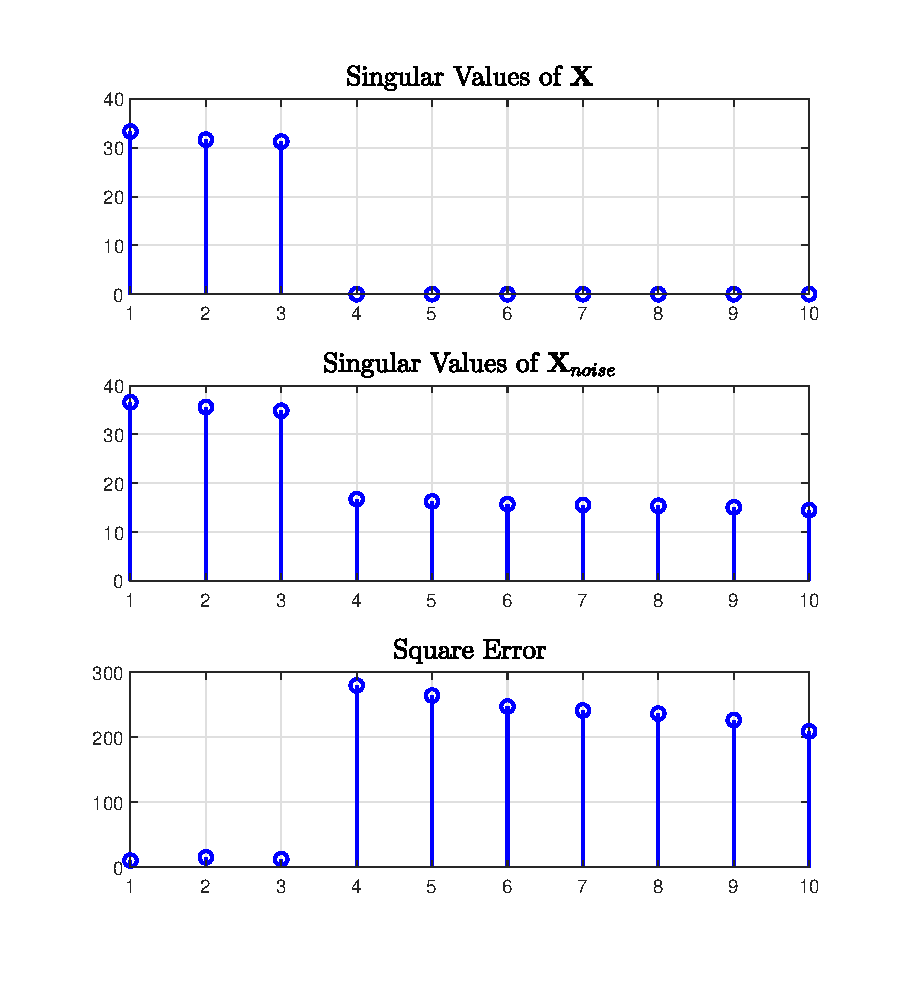
\includegraphics[width=0.48\textwidth]{fig/1.6_1.eps}
        \label{fig11a}
	}
    \subfigure[Singular values of the denoised matrix (top). The mean square error between the columns of the noiseless input matrix and the noisy and denoise matrices (bottom).]{
		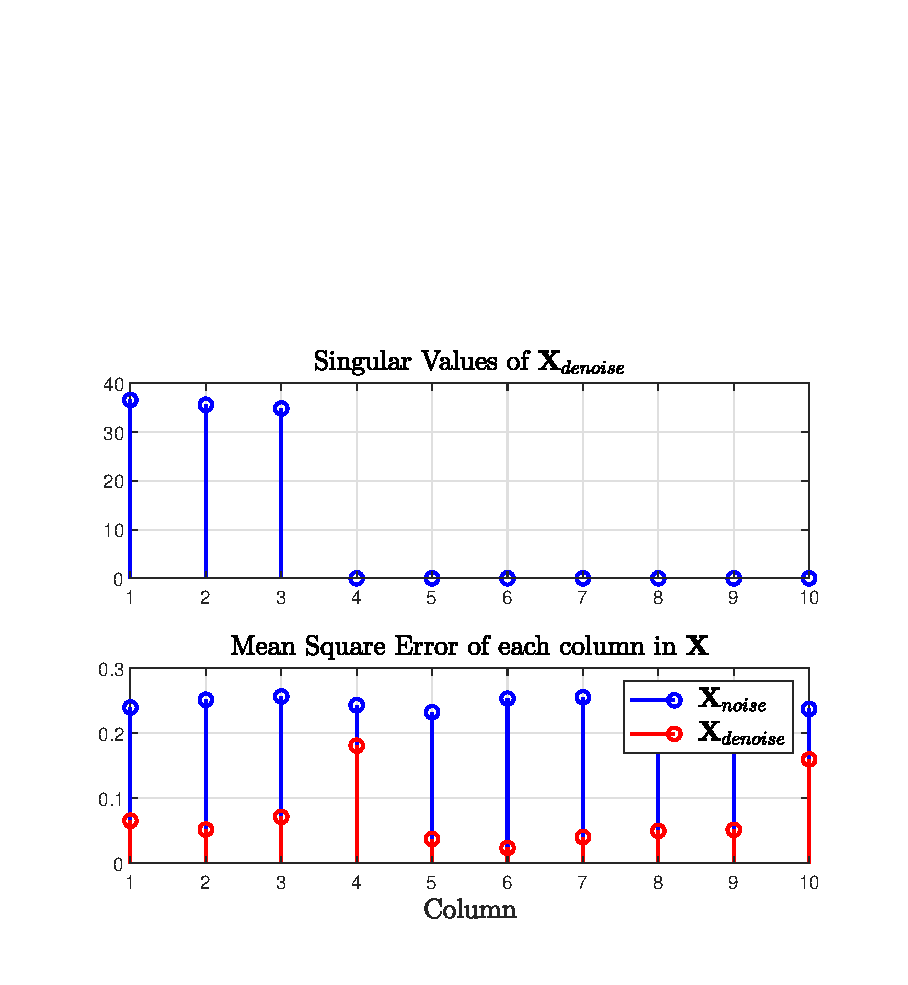
\includegraphics[width=0.48\textwidth]{fig/1.6_2.eps}
        \label{fig11b}
    }
    \caption{Analysis of the singular values of different data matrices}
    \label{fig11}
\end{figure}

\subsection{Robust Regression}

\subsubsection{Task a \& b: Denoised Matrix}
\ \indent
Figure \ref{fig11a} shows the singular values of the $\mathbf{X}$ and 
$\mathbf{X}_{noise}$ and the square errors between them. 
From the singular values of both $\mathbf{X}$ and $\mathbf{X}_{noise}$, 
it can be identified that the rank of the input data is 3, as the first 3 
singular values are much larger than the rest. From the square error 
plotting, it is noticeable that the effect of the noise on the singular 
values is that it enlarges the zero singular values in the original input 
data. Therefore, if the noise makes all the singular values have the same 
value level, it becomes hard to identify the rank of the noisy matrix 
$\mathbf{X}_{noise}$.

The $\mathbf{X}_{noise}$ can be denoised using only the r (rank of the
 matrix) most significant principal components. The denoised low-rank 
 matrix ${\tilde{{\bf{X}}}}_{noise}$ is given by
 \begin{equation}
	{\tilde{{\bf{X}}}}_{noise}={\tilde{{\bf{U}}}\left(:,1:r\right)\tilde{{\bf{S}}}\left(1:r,1:r\right)\tilde{{\bf{V}}}}^H\left(:,1:r\right)
 \end{equation}
 where $\tilde{\bf{U}}$, $\tilde{{\bf{S}}}$, and $\tilde{{\bf{V}}}$ are obtained by 
 SVD of the $\mathbf{X}_{noise}$, i.e.,
 \begin{equation}
	\mathbf{X}_{noise}=\tilde{{\bf{U}}} \tilde{\bf{S}} \tilde{{\bf{V}}}^H
 \end{equation}

Figure \ref{fig11b} shows the singular values of the denoised matrix 
${\tilde{\mathbf{X}}}_{noise}$, and indicates that this operation
is capable of reducing the error with the noiseless data.

\subsubsection{Task c \& d: OLS and PCR}
\ \indent
Table \ref{table1} shows the mean square error of the ${\hat{{\bf{Y}}}}_{\text{OLS}}$ and 
${\hat{{\bf{Y}}}}_{\text{PCR}}$ with the $\bf{Y}$ on the provided training set and testing set. 
The last column of this table shows the averaged mean square error on the 
1000 different testing sets. 

In the training set, the OLS has a better performance than PCR on the 
training set, while has a worse performance than PCR on the testing set.
 The reason is that the OLS method also captures some noise characters, 
 leading to overfit of the model on the training set. By testing the OLS 
 and PCR model on 1000 different testing sets, we can conclude that the 
 PCR method is more efficient on the out-of-sample data.

\begin{table}[htbp]
	\caption{Comparison of OLS and PCR methods}
	\centering
    \setlength{\tabcolsep}{8mm}{
        \centering
        \begin{tabular}{lll}% 通过添加 | 来表示是否需要绘制竖线
            \toprule
             &OLS & PCR\\\hline

            Training set & 0.7103 & 0.7154\\

            Testing set & 0.4755 & 0.4708\\

            1000 testing set & 0.4711 & 0.4674\\

            \bottomrule
        \end{tabular} \label{table1}
    }
\end{table}

\newpage
\section{Adaptive Signal Processing}

\subsection{The Least Mean Square (LMS) Algorithm}

\subsubsection{Task a: Convergence in Mean}
\ \indent
The following 2-order AR process is considered
\begin{equation}
	x(n) = a_1 x(n-1) + a_2 x(n-2) + \eta(n) \label{eq22}
\end{equation}
where $\eta(n) \sim \mathcal{N}(0, \sigma_{\eta}^2)$ is the Gaussian noise power.
In order to estimate the coefficients $a_1$ and $a_2$ using LMS, the input vector is 
${\bf{x}}(n) = [x(n-1), x(n-2)]^T$. Its correlation matrix is given as
\begin{align}
	{\bf{R}} & = \mathbb{E} \left\{ {\bf{x}}(n) {\bf{x}}^T(n) \right\} = \left[\begin{matrix}
		\mathbb{E} \left\{ x(n-1) x(n-1) \right\} & \mathbb{E} \left\{ x(n-1) x(n-2) \right\} \\
		\mathbb{E} \left\{ x(n-2) x(n-1) \right\} & \mathbb{E} \left\{ x(n-2) x(n-2) \right\}	\end{matrix}\right]	= \left[ \begin{matrix}
		r_{xx}(0) & r_{xx}(1)\\
		r_{xx}(1) & r_{xx}(0)
	\end{matrix} \right]
\end{align}
The entries of the correlation matrix can be calculated by a set of 3 linear equtions
\begin{equation}
	\left[
		\begin{matrix}
			r_{xx}(0) & r_{xx}(1) & r_{xx}(2)\\
			r_{xx}(1) & r_{xx}(0) & r_{xx}(1)\\
			r_{xx}(2) & r_{xx}(1) & r_{xx}(0)
		\end{matrix}
	\right] 
	\left[
		\begin{matrix}
			1 \\ a_1 \\ a_2
		\end{matrix}
	\right]
	= \left[
		\begin{matrix}
			\sigma_{\eta}^2 \\ 0 \\ 0
		\end{matrix}
	\right] \label{eq24}
\end{equation}
If the original parameters are $a_1=0.1$, $a_2=0.8$ and $\sigma_{\eta}^2=0.25$,
the solution of \eqref{eq24} is $r_{xx}(0) = 0.6966$, $r_{xx}(1)=-0.0387$ and $r_{xx}(2) = -0.5534$.
Therefore, the correlation matrix is 
\begin{equation}
	{\bf{R}} = \left[
		\begin{matrix}
			0.6966 & -0.0387 \\
			-0.0387 & 0.6966
		\end{matrix}
	\right] \label{eq25}
\end{equation}

Denote the estimated AR coefficients at step $n$ by ${\bf{w}}(n) = [\hat{a}_1(n), \hat{a}_2(n)]^T$.
The LMS algorithm will minimize the cost function $J(n)=\frac{1}{2} e^2(n)$ by updating ${\bf{w}}(n)$
according to
\begin{eqnarray}
	{\bf{w}}(n+1) = {\bf{w}}(n) + \mu e(n) {\bf{x}}(n) \label{eq26}  
\end{eqnarray}
where $e(n) = x(n) - {\bf{w}}^T(n){\bf{x}}(n)$. To ensure the convergence of the LMS in mean, 
the step size $\mu$ needs to stisfy 
\begin{equation}
	0 < \mu < \frac{2}{\text{Tr}\{{\bf{R}}\}} \label{eq27}
\end{equation}
where $\text{Tr}\{{\bf{R}}\}$ is trace of the covariance matrix ${\bf{R}}$Therefore, the range of the step size $\mu$ is
\begin{equation}
	0 < \mu < 1.44 \label{eq28}
\end{equation}


\begin{figure}[htbp]
    \centering
	\subfigure[$\mu = 0.05$]{
		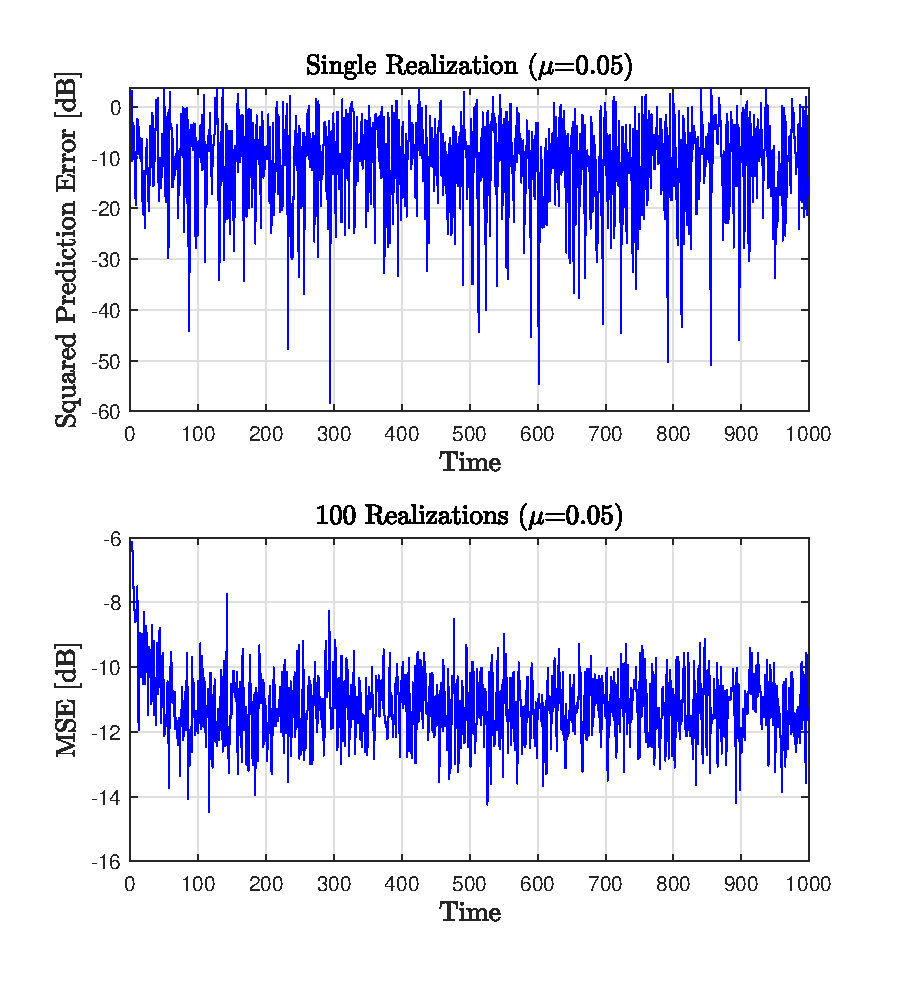
\includegraphics[width=0.48\textwidth]{fig/2.1_1.eps}
        \label{fig12a}
	}
    \subfigure[$\mu = 0.01$]{
		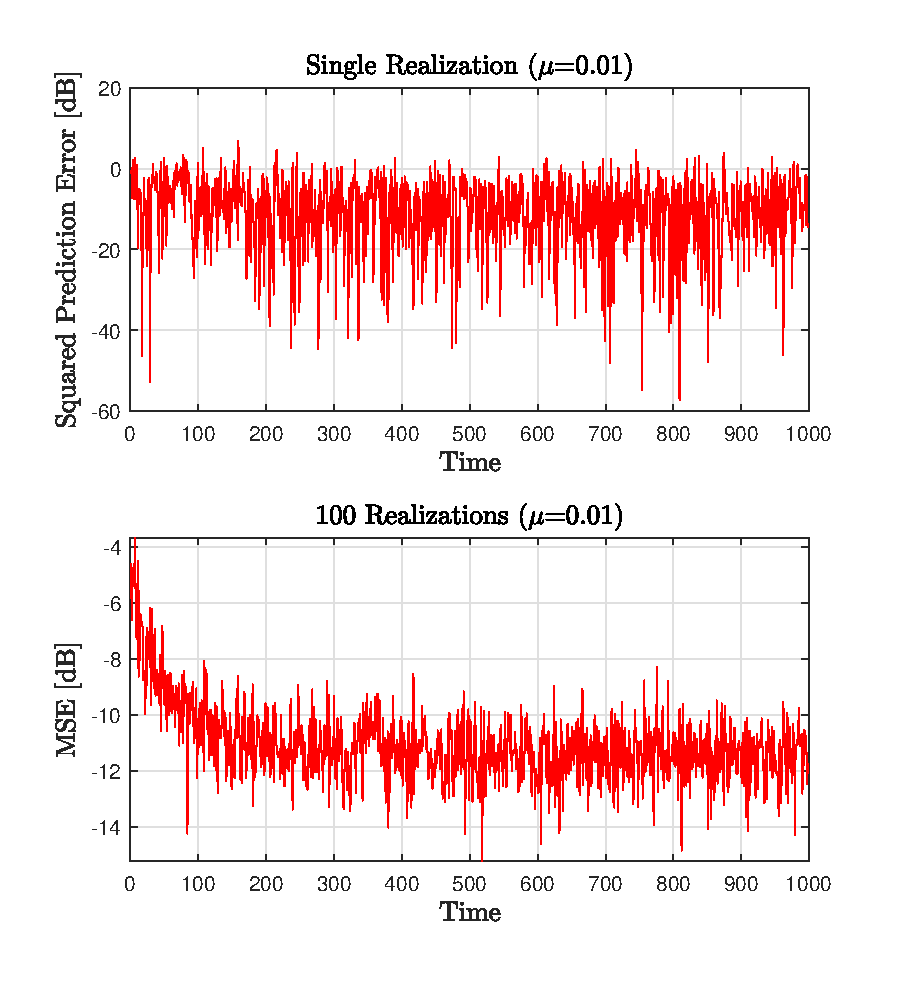
\includegraphics[width=0.48\textwidth]{fig/2.1_2.eps}
        \label{fig12b}
    }
    \caption{The value of the $e^2(n)$ (dB) (top) and the average $e^2(n)$ (dB) of 100 different realizations (bottom)}
    \label{fig12}
\end{figure}

\subsubsection{Task b: Step Size}
\ \indent
Figure \ref{fig12} shows the squared error and average squared error (over 100 realizations) with 
step size of 0.05 and 0.01, respectively. According to the learning curve (plots of the average square error),
the LMS starts to converge at around 100 steps when $\mu=0.05$ while it starts to converge at around 200 steps 
when $\mu=0.01$, which indicates that the LMS can converge faster when the step size is larger.

\subsubsection{Task c \& d: Excess Error}

\ \indent
For small step-size, the misadjustment of the LMS is approximated as
\begin{equation}
	\mathcal{M}_{\text{LMS}} \approx \frac{\mu}{2} \text{Tr}\{{\bf{R}}\} \label{eq29}
\end{equation}
According to the result in \eqref{eq25}, the theoretical misadjustment for $\mu=0.05$ 
and $\mu=0.01$ should be $\mathcal{M}_{0.05} \approx 0.035$ and $\mathcal{M}_{0.01} \approx 0.007$, 
respectively.

The estimated misadjustment is obtained by time-averaging over the steady state of the
ensemble-averaged learning curves using 100 independent trials of the experiment. For both $\mu=0.05$ and
$\mu=0.01$, 10 estimated values of misadjustment are calculated by repeating the aforementioned process 10
times, which are shown below
\begin{align}
	\hat{\mathcal{M}}_{0.05} = [\begin{matrix}
		0.040 &0.045 &0.054 &0.039 &0.050 &0.068 &0.055 &0.051 &0.059 &0.061
	\end{matrix}] \\
	\hat{\mathcal{M}}_{0.01} = [\begin{matrix}
		0.014 &0.018 &0.016 &0.006 &0.022 &0.004 &0.013 &0.021 &0.007 &0.014
	\end{matrix}]
\end{align}
According to the estimated results, we can see that the estimated misadjustment is usually larger that 
the theoretical one. However, for the smaller step size (i.e., $\mu=0.01$), the estimates are closer to
the theoretical values.

The estimated AR coefficients $\hat{a}_1$ and $\hat{a}_2$ are also obtained by averaging the steady-state values of 100
trials of the experiment, which are shown in Table \ref{table2}. It is obvious that for the smaller 
step size (i.e.,$\mu=0.01$), the estimated coefficients have smaller error. The reason is that
the smaller step size leads to the smaller excess error.


\begin{table}[htbp]
	\caption{Comparison of estimated AR coefficients using different step size}
	\centering
    \setlength{\tabcolsep}{8mm}{
        \centering
        \begin{tabular}{ccc}% 通过添加 | 来表示是否需要绘制竖线
            \toprule
            Value & $\mu=0.05$ & $\mu=0.01$\\\hline

            $\hat{a}_1$ & 0.071 & 0.111\\

            $\hat{a}_2$ & 0.716 & 0.748\\

			$|\hat{a}_1 - a_1|$ & 0.029 & 0.011\\

			$|\hat{a}_2 - a_2|$ & 0.084 & 0.052\\
            \bottomrule
        \end{tabular} \label{table2}
    }
\end{table}

\subsubsection{Task e \& f: The Leaky LMS Algorithm}
\ \indent
In order to derive the Leaky LMS coefficient update for ${\bf{w}}(n)$, we can 
first consider the Steepest Descent methods, where the following cost function is minimized
\begin{align}
	\tilde{J}_2(n) & = \mathbb{E} \{ J_2(n) \} \nonumber \\
	& = \frac{1}{2} \mathbb{E} \left\{ e^2(n) + \gamma \Vert {\bf{w}}(n) \Vert_2^2 \right\} \nonumber \\
	& = \frac{1}{2} \mathbb{E} \left\{ e^2(n) \right\} + \frac{1}{2} \gamma \Vert {\bf{w}}(n) \Vert_2^2 \nonumber \\
	& = \frac{1}{2} \mathbb{E} \left\{ \left( x(n) - {\bf{w}}^T(n) {\bf{x}}(n) \right) \left( x(n) - {\bf{w}}^T(n) {\bf{x}}(n) \right)^T  \right\} + \frac{1}{2} \gamma {\bf{w}}^T(n) {\bf{w}}(n) \nonumber \\
	& = \frac{1}{2} \mathbb{E} \left\{ x^2(n) - 2 x(n) {\bf{x}}^T(n) {\bf{w}}(n) + {\bf{w}}^T(n) {\bf{x}}(n) {\bf{x}}^T(n) {\bf{w}}(n) \right\} + \frac{1}{2} \gamma {\bf{w}}^T(n) {\bf{w}}(n) \nonumber \\
	& = \frac{1}{2} \left( \underbrace{\mathbb{E} \{x^2(n) \}}_{\sigma_x^2} - 2 {\bf{w}}^T(n) \underbrace{\mathbb{E} \{ {\bf{x}}(n)x(n) \}}_{\bf{p}} + {\bf{w}}^T(n) \underbrace{\mathbb{E} \{ {\bf{x}}(n) {\bf{x}}^T(n) \}}_{\bf{R}} {\bf{w}}(n) \} \right) + \frac{1}{2} \gamma {\bf{w}}^T(n) {\bf{w}}(n) \nonumber \\
	& = \frac{1}{2} \sigma_x^2 - {\bf{w}}^T(n) {\bf{p}} + \frac{1}{2} {\bf{w}}^T(n) {\bf{R}} {\bf{w}}(n) + \frac{1}{2} \gamma {\bf{w}}^T(n) {\bf{w}}(n)
\end{align}
In Steepest Descent, ${\bf{w}}(n)$ is updated in the direction of the negative gradient of cost function $\tilde{J}_2(n)$. The gradient is given as 
\begin{align}
	\nabla \tilde{J}_2(n) |_{{\bf{w}}(n)} & = -{\bf{p}} + \frac{1}{2} \left( {\bf{R}} + {\bf{R}}^T \right) {\bf{w}}(n) + \gamma {\bf{w}}(n) \nonumber \\
	& = -{\bf{p}} + {\bf{R}} {\bf{w}}(n) + \gamma {\bf{w}}(n)
\end{align}
Therefore, the coefficient update in Steepest Descent methods is 
\begin{align}
	{\bf{w}}(n+1) & = {\bf{w}}(n) + \mu \left( -\nabla \tilde{J}_2(n) |_{{\bf{w}}(n)} \right) \nonumber \\
	& = {\bf{w}}(n) + \mu \left( {\bf{p}} - {\bf{R}} {\bf{w}}(n) - \gamma {\bf{w}}(n) \right) \nonumber \\
	& = (1 - \mu \gamma) {\bf{w}}(n) + \mu ({\bf{p}} - {\bf{R}} {\bf{w}}(n)) \label{eq34}
\end{align}

In the LMS, we replace ${\bf{p}}$ and $\bf{R}$ by the instantaneous estimate, i.e., $\hat{\bf{p}} = {\bf{x}}(n) x(n)$
and $\hat{\bf{R}} = {\bf{x}}(n) {\bf{x}}^T(n)$. The coefficient update in \eqref{eq34} is converted to 
\begin{align}
	{\bf{w}}(n+1) & = (1 - \mu \gamma) {\bf{w}}(n) + \mu (\hat{\bf{p}} - \hat{\bf{R}} {\bf{w}}(n)) \nonumber \\
	& = (1 - \mu \gamma) {\bf{w}}(n) + \mu ({\bf{x}}(n) x(n) - {\bf{x}}(n) {\bf{x}}^T(n) {\bf{w}}(n)) \nonumber \\
	& = (1 - \mu \gamma) {\bf{w}}(n) + \mu {\bf{x}}(n) \underbrace{\left( x(n) - {\bf{x}}^T(n) {\bf{w}}(n) \right)}_{e(n)} \nonumber \\
	& = (1 - \mu \gamma) {\bf{w}}(n) + \mu e(n) {\bf{x}}(n) \label{eq35}
\end{align}
We get the coefficient update \eqref{eq35} for leaky LMS.

The leaky LMS is implemented to estimated AR coefficients of \eqref{eq22}, where $a_1=0.1$
and $a_2 = 0.8$. Table \ref{table3} and Table \ref{table4} show the estimates of 
$a_1$ and $a_2$, respectively. 

\begin{table}[htbp]
	\caption{Estimates of $a_1$ using different $\mu$ and $\gamma$}
	\centering
    \setlength{\tabcolsep}{8mm}{
        \centering
        \begin{tabular}{lcc}% 通过添加 | 来表示是否需要绘制竖线
            \toprule
            & $\mu=0.05$ & $\mu=0.01$\\\hline

            $\gamma=0.01$ & 0.073 & 0.112\\

            $\gamma=0.1$ & 0.091 & 0.128\\

			$\gamma=5$ & 0.047 & 0.058\\

			$\gamma=10$ & 0.031 & 0.035\\

            \bottomrule
        \end{tabular} \label{table3}
    }
\end{table}

\begin{table}[htbp]
	\caption{Estimates of $a_2$ using different $\mu$ and $\gamma$}
	\centering
    \setlength{\tabcolsep}{8mm}{
        \centering
        \begin{tabular}{lcc}% 通过添加 | 来表示是否需要绘制竖线
            \toprule
            & $\mu=0.05$ & $\mu=0.01$\\\hline

            $\gamma=0.01$ & 0.705 & 0.736\\

            $\gamma=0.1$ & 0.619 & 0.663\\

			$\gamma=5$ & 0.105 & 0.114\\

			$\gamma=10$ & 0.060 & 0.063\\
            \bottomrule
        \end{tabular} \label{table4}
    }
\end{table}

For the fixed $\gamma$, the smaller $\mu$ still results in the 
better estimates.For fixed $\mu$, with the increase of the $\gamma$, the leaky LMS converge to
incorrect values of the coefficients, which approach zero. This can be explained in two perspectives.
\begin{itemize}
	\item In the perspective of the cost function, there is an additional term $\gamma \Vert {\bf{w}}(n) \Vert^2$
	in leaky LMS. If we reduce the cost function, we will also reduce the norm of the coefficients ${\bf{w}}$.
	Therefore, for the large $\gamma$, the term $\gamma \Vert {\bf{w}}(n) \Vert^2$ will become dominant in the cost
	function, which means we are mainly minimizing the norm of the coefficients. In this case, we will get the small
	coefficient, which is incorrect.
	\item In the perspective of the coefficient update in \eqref{eq35}, we can consider the model of convergence. 
	We define the distance vector ${\bf{v}}(n) = {\bf{w}}(n) - {\bf{w}}_{\text{opt}}$ and rewrite \eqref{eq22} as
	$x(n) = {\bf{x}}^T(n) {\bf{w}}_{\text{opt}} + \eta(n)$. In this case, we can rewrite \eqref{eq35} as
	\begin{align}
		{\bf{w}}(n+1) & = (1-\mu \gamma) {\bf{w}}(n) + \mu {\bf{x}}(n) \left( {\bf{x}}^T(n) {\bf{w}}_{\text{opt}} + \eta(n) - {\bf{x}}^T(n) {\bf{w}}(n) \right) \nonumber \\
		& = (1-\mu \gamma) {\bf{w}}(n) + \mu {\bf{x}}(n) {\bf{x}}^T(n) {\bf{w}}_{\text{opt}} - \mu {\bf{x}}(n) {\bf{x}}^T(n) {\bf{w}}(n) + \mu {\bf{x}}(n) \eta(n)
	\end{align}
	By subtracting ${\bf{w}}_{\text{opt}}$ from both sides, we get 
	\begin{align}
		{\bf{v}}(n+1) & = (1-\mu \gamma) {\bf{v}}(n) - \mu {\bf{x}}(n) {\bf{x}}^T(n) {\bf{v}}(n) + \mu {\bf{x}}(n) \eta(n) \\
		\mathbb{E} \left\{ {\bf{v}}(n+1) \right\} &= \left( (1-\mu \gamma) {\bf{I}} - \mu \mathbb{E}\{{\bf{x}}(n) {\bf{x}}^T(n)\} \right) \mathbb{E} \{ {\bf{v}}(n) \} + \mu \mathbb{E}\{ \eta(N) {\bf{x}}(n) \} \nonumber \\
		& =  \left( (1-\mu \gamma) {\bf{I}} - \mu {\bf{R}} \right) \mathbb{E} \{ {\bf{v}}(n) \} \label{eq38}
	\end{align}
	We define the transformed vector $\tilde{\bf{v}}(n) = {\bf{Q}} {\bf{v}}(n)$, where $\bf{Q}$ is obtained from the eigenvalue decomposition of
	${\bf{R}}$, i.e., ${\bf{R}} = {\bf{Q}} {\bf{\Lambda}} {\bf{Q}}^T$. Then we can rewrite \eqref{eq38} as
	\begin{gather}
		\tilde{\bf{v}}(n+1) = ((1-\mu \gamma) {\bf{I}} - \mu {\bf{\Lambda}}) \tilde{\bf{v}}(n) \\
		\left[\begin{matrix}
			\tilde{v}_1(n+1) \\
			\vdots\\
			\tilde{v}_1(n+1)
		\end{matrix}\right] = 
		\left[\begin{matrix}
			1 - \mu \gamma - \mu \lambda_{max} & 0 & \cdots & 0\\
			0 & 1 - \mu \gamma - \mu \lambda_2 & \cdots & 0\\
			\vdots & \vdots & \ddots & \vdots\\
			0 & 0 & \cdots & 1 - \mu \gamma - \mu \lambda_{min}
		\end{matrix}\right] \left[\begin{matrix}
			\tilde{v}_1(n) \\
			\vdots\\
			\tilde{v}_1(n)
		\end{matrix}\right]
	\end{gather}
	In order to ensure the convergence of the leaky LMS, we need to guarantee that 
	$|1 - \mu \gamma - \mu \lambda_i| < 1$. Because of the term $- \mu \gamma$, it can be guaranteed 
	even though one of the eigenvalues $\lambda_i$ is zero, which is the aim of leaky LMS. However, for the 
	large $\gamma$, it can be regarded as the distance ${\bf{v}}(n)$ is reduced in a large rate,
	which is equivalent to using large step size. Therefore, there will be large excess error when the large $\gamma$ is used,
	resulting in the incorrect estimates of coefficients.

\end{itemize}

\subsection{Adaptive Step Sizes}
\subsubsection{Task a: GASS Algorithm}
\ \indent
In the gradient adaptive step-size (GASS) algorithms, the step size of LMS is 
dynamically updated at each step according to
\begin{equation}
	\mu(n+1) = \mu(n) + \rho e(n) {\bf{x}}^T(n) \psi (n)
\end{equation}
where the $\psi(n)$ can be calculated following three methods
\begin{align}
	{\text{Benveniste:}} \quad & \psi(n) = \left[{\bf{I}} - \mu(n-1) {\bf{x}}(n-1) {\bf{x}}^T(n-1) \right] \psi(n-1) + e(n-1) {\bf{x}}(n-1) \\
	{\text{Farhang:}} \quad & \psi(n) = \alpha \psi(n-1) + e(n-1) {\bf{x}}(n-1), \quad 0 < \alpha < 1\\
	{\text{Matthews:}} \quad & \psi(n) = e(n-1) {\bf{x}}(n-1)
\end{align}

In this part, the following real-value MA(1) process is considered.
\begin{equation}
	x(n) = 0.9 \eta(n-1) + \eta(n), \quad \eta \sim \mathcal{N}(0, 0.5) \label{eqMA}
\end{equation}

\begin{figure}[htbp]
    \centering
	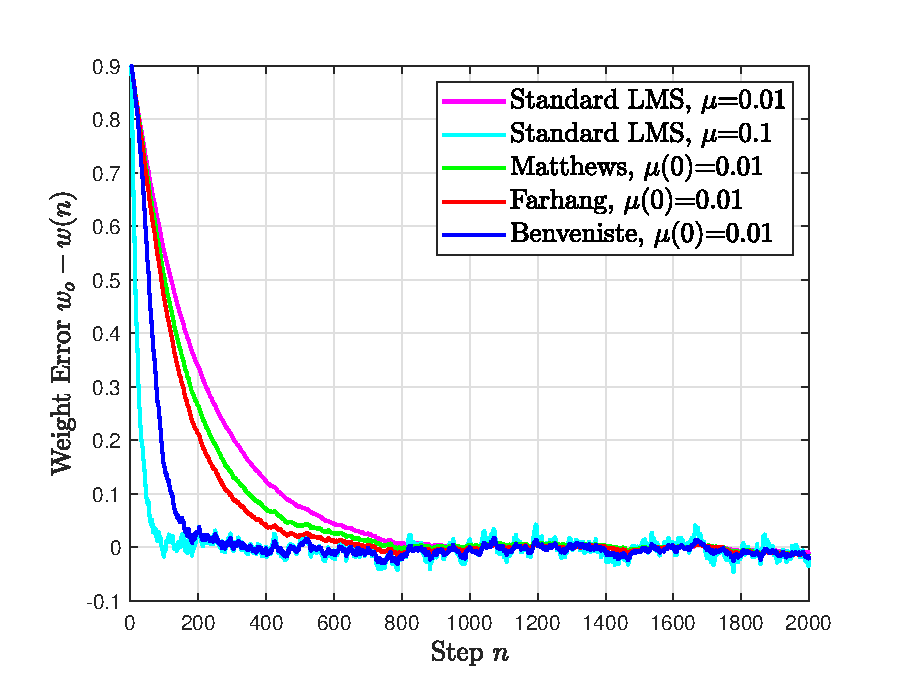
\includegraphics[width=0.6\textwidth]{fig/2.2_1_alter.eps}

    \caption{Comparison of standard LMS and GASS algorithm}
    \label{fig13}
\end{figure}

The standard LMS and GASS algorithms are implemented in the system identification setting 
to identify the MA(1) system in \eqref{eqMA}. The input to the LMS is ${\bf{x}}(n) = [\eta(n-1)]^T$.
The expression of error is $e(n) = x(n) - {\bf{w}}^T(n){\bf{x}}(n)$. The standard LMS is 
implemented with step size of $\mu=0.01$ and $\mu=0.1$. For GASS algorithms, theri 
initial step sizes for weights update are all set to $\mu(0)=0.01$, and the step size 
for $\mu(n)$ update is set to $\rho=0.0005$.

Figure \ref{fig13} shows the weight error in the standard LMS and GASS algorithms. The curves are
plotted by averaging 100 trials of experiments. We can see that the standard LMS with $\mu=0.1$ congerges
fastest, but it has the largest steady state error. Benveniste's method also converge fast, which is only
a little slower than standard LMS with $\mu=0.1$, although its $\mu$ starts from a small value. 
Compared with standard LMS with $\mu=0.1$, Benveniste’s method has smaller steady state error. Both 
Farhang's and Matthews's method converge slower than the Benveniste’s method, but they have better 
performance in terms of steady state error. The standard LMS with $\mu=0.01$ converge slowest and its 
steady state error is also smaller than Benveniste’s method.

In conclusion, the GASS outperforms LMS in terms of the convergence speed, but it may lead to higher steady
state error.



% Based on the duality of AR and MA processes, this MA(1) process can be transformed to 
% an AR process with infinite order, which is shown below.
% \begin{equation}
% 	x(n) = \lim_{M \to \infty} \sum_{m=1}^M 0.9^m x(n-m) + \eta(n) \label{eqAR}
% \end{equation}
% Therefore, the finite length version of \eqref{eqAR} is taken to approximate the MA(1) process. In the LMS algorithm,
% then input will be ${\bf{x}}(n) = [x(n-1),...,x(n-M)]^T$, and the weight of $x(n-1)$ will close to the weight of MA(1) process.

% The next step is to determine the rang of step size $\mu$. Consider the correlation matrix of ${\bf{x}}(n)$, which is
% \begin{equation}
% 	{\bf{R}} = \mathbb{E} \{ {\bf{x}}(n) {\bf{x}}^T(n) \} = \left[ \begin{matrix}
% 		\mathbb{E} \{ x(n-1)x(n-1) \} & \cdots & \mathbb{E} \{ x(n-1)x(n-M) \}\\
% 		\vdots & \ddots & \vdots \\
% 		\mathbb{E} \{ x(n-M)x(n-1) \} & \cdots & \mathbb{E} \{ x(n-M)x(n-M) \}
% 	\end{matrix} \right]
% \end{equation}
% The range of $\mu$ is given as 
% \begin{gather}
% 	0 < \mu < \frac{2}{\text{Tr}\{\bf{R}\}}\\
% 	\text{Tr}\{{\bf{R}}\} = \sum_{m=1}^M \mathbb{E} \{ x(n-m)x(n-m) \} = 0.905 M
% \end{gather}

% In order to make both $\mu=0.1$ and $\mu=0.01$ achievable, $M=4$ is chosen in this part. Furthermore, for GASS,
% the leaning rate of $\mu(n)$ is set to $\rho=0.00005$ and the value of $\alpha$ in Farhang's method is set to $\alpha=0.5$.

% \begin{figure}[htbp]
%     \centering
% 	\subfigure[$\mu = 0.1$]{
% 		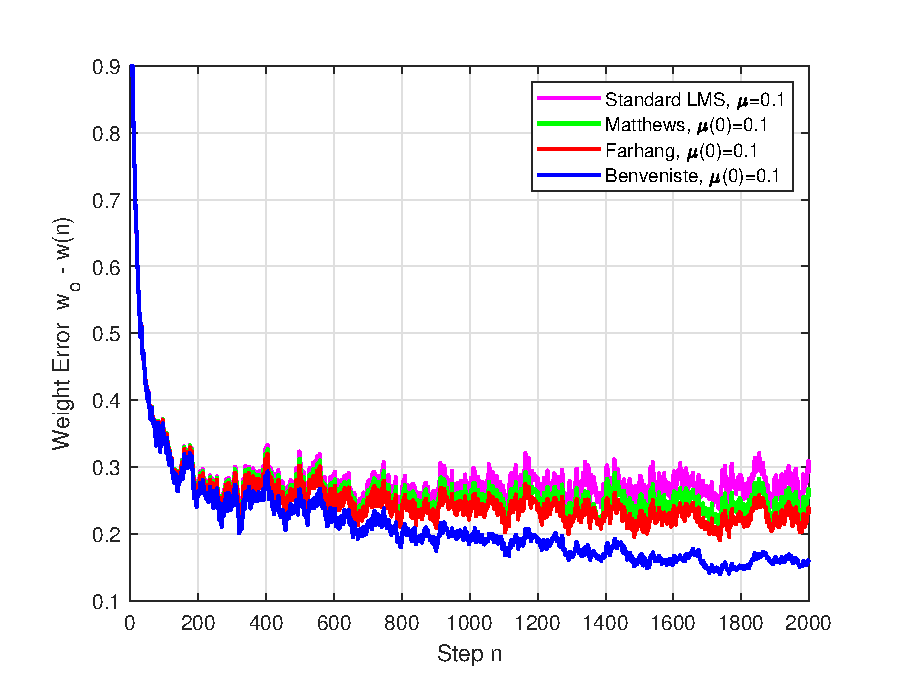
\includegraphics[width=0.48\textwidth]{fig/2.2_1.eps}
%         \label{fig13a}
% 	}
%     \subfigure[$\mu = 0.01$]{
% 		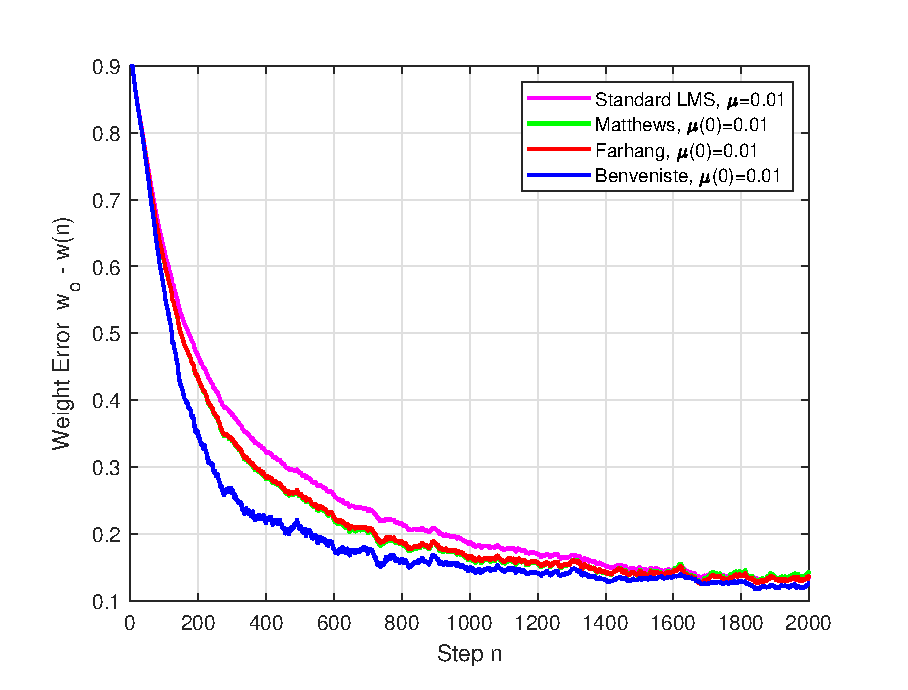
\includegraphics[width=0.48\textwidth]{fig/2.2_2.eps}
%         \label{fig13b}
%     }
%     \caption{Comparison of standard LMS and GASS algorithm}
%     \label{fig13}
% \end{figure}

% Figure \ref{fig13} shows the weight error curves by averaging the results of 100 trials of experiments.
% We can see that the GASS algorithms usually converge faster that the standard LMS algorithm, in which the 
% Benveniste's method converge fastest. Apart from the convergence speed, GASS algorithms also outperform standard LMS
% in terms of steady state error. In the case of $\mu=0.01$, both GASS and standard LMS are converged to a relative small steady error.
% For $\mu=0.1$, both Matthews's and Farhang's methods outperforms the standard LMS, but they have a relative large steady state error.
% However, for Benveniste's method, it can still converge to a small weight error (even close to the case $\mu=0.01$), and it steady state error is
% also very small.

\subsubsection{Task b: NLMS Algorithm}
\ \indent
In the normalized LMS (NLMS), the coefficients update is 
\begin{equation}
	{\bf{w}}(n+1) = {\bf{w}}(n) + \frac{\beta}{\epsilon + \Vert {\bf{x}}(n) \Vert ^2} e(n) {\bf{x}}(n) \label{eq41}
\end{equation}
which can be equivalently written in the form of 
\begin{equation}
	{\bf{w}}(n+1) = {\bf{w}}(n) + \mu e_p(n) {\bf{x}}(n) \label{eq42}
\end{equation}
where $e_p(n) = d(n) - {\bf{x}}^T(n) {\bf{w}}(n+1)$.
\begin{proof}
	Firstly, define $\Delta {\bf{w}}(n) = {\bf{w}}(n+1) - {\bf{w}}(n)$, then we have
	\begin{align}
		\Delta{\bf{w}}(n) & = {\bf{w}}(n+1) - {\bf{w}}(n) \nonumber \\
		& = \mu e_p(n) {\bf{x}}(n) \\
		& = \mu \left( d(n) - {\bf{x}}^T(n) \left( {\bf{w}}(n) + \Delta {\bf{w}}(n) \right) \right) {\bf{x}}(n) \nonumber \\
		& = \mu ( \underbrace{d(n) - {\bf{x}}^T(n) {\bf{w}}(n)}_{e(n)} -{\bf{x}}^T(n)  \Delta {\bf{w}}(n)  ) {\bf{x}}(n) \nonumber \\
		& = \mu \left( e(n) - {\bf{x}}^T \Delta{\bf{w}}(n) \right) {\bf{x}}(n) \nonumber \\
		& = \mu e(n) {\bf{x}}(n) - \mu {\bf{x}}^T(n) {\bf{x}}(n) \Delta {\bf{w}}(n)
	\end{align}
	By rearrange this expression, we have
	\begin{align}
		( 1 + \mu {\bf{x}}^T(n) {\bf{x}}(n)) \Delta {\bf{w}}(n) & = \mu e(n) {\bf{x}}(n)\\
		\Delta {\bf{w}}(n) &= \frac{\mu}{1 + \mu \Vert {\bf{x}}(n) \Vert^2} e(n) {\bf{x}}(n) \nonumber \\
		& = \frac{1}{\frac{1}{\mu} + \Vert {\bf{x}}(n) \Vert^2} e(n) {\bf{x}}(n)
	\end{align}

	By setting $\beta=1$ and $\epsilon = 1 / \mu$, we get
	\begin{align}
		{\bf{w}}(n+1) & = {\bf{w}}(n) + \Delta {\bf{w}}(n) \nonumber \\
		& = {\bf{w}}(n) + \frac{\beta}{\epsilon + \Vert {\bf{x}}(n) \Vert^2} e(n) {\bf{x}}(n)
	\end{align}
	Therefore, we prove that the \eqref{eq42} is equivalent to \eqref{eq41} with $\beta=1$ and $\epsilon=1/ \mu$.
 $\hfill\blacksquare$ 
\end{proof}

\subsubsection{Task c: GNGD Algorithm}
\ \indent
In Generalized Normalized Gradient Descent (GNGD) algorithm, the regularization facotr in NLMS is 
updated according to
\begin{equation}
	\epsilon (n+1) = \epsilon (n) - \rho \mu \frac{ e(n) e(n-1) {\bf{x}}^T(n) {\bf{x}}(n-1) }{ \left( \epsilon(n-1) + \Vert  {\bf{x}}(n-1) \Vert^2 \right)^2 }
\end{equation} 

\begin{figure}[htbp]
    \centering
	\subfigure[$\mu = 0.01$]{
		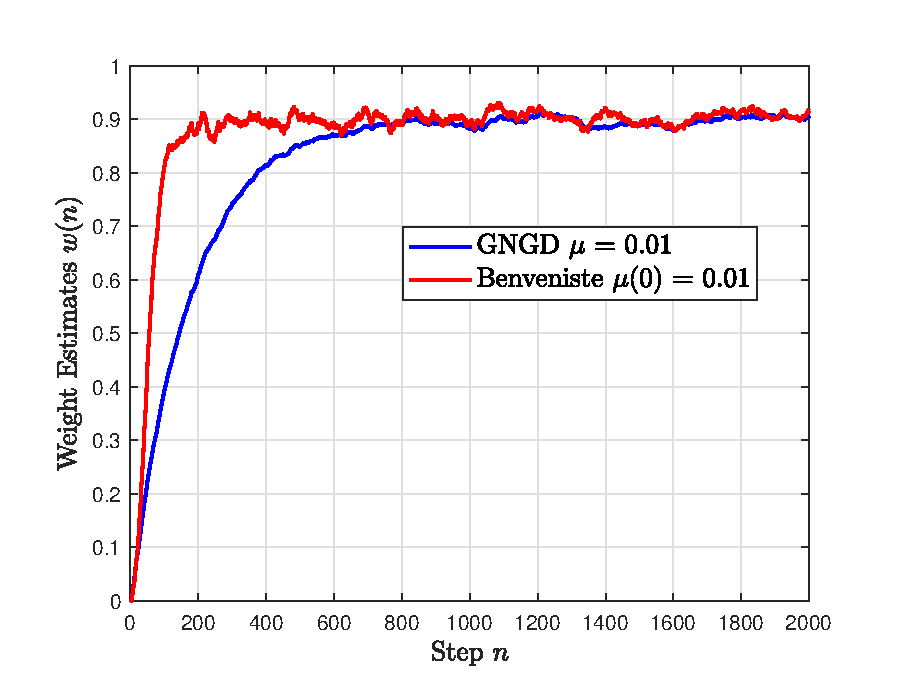
\includegraphics[width=0.48\textwidth]{fig/2.2_2_alter.eps}
        \label{fig14a}
	}
    \subfigure[$\mu = 0.1$]{
		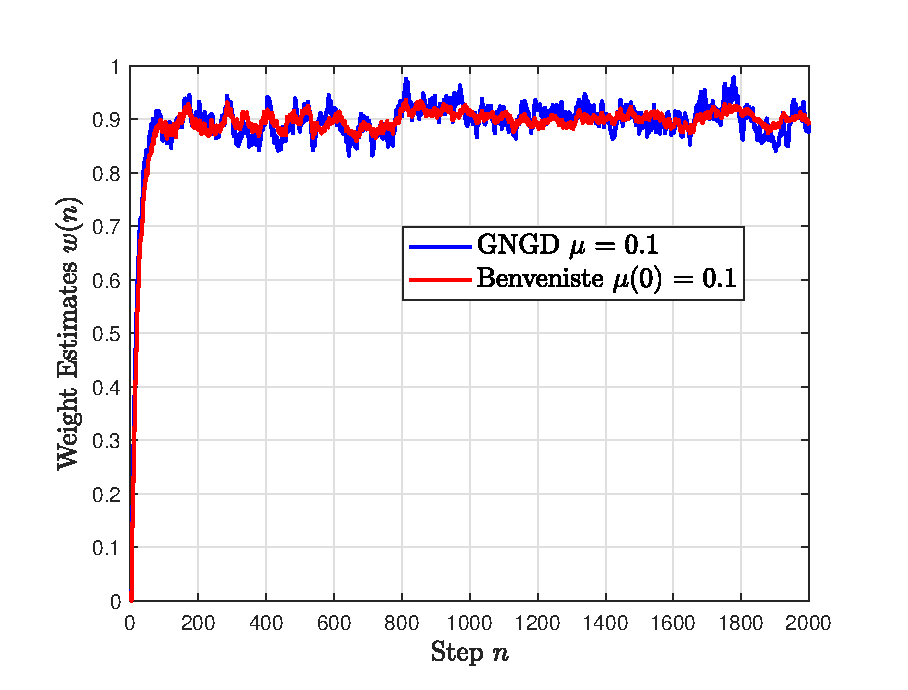
\includegraphics[width=0.48\textwidth]{fig/2.2_3_alter.eps}
        \label{fig14b}
    }
	\subfigure[$\mu = 1$]{
		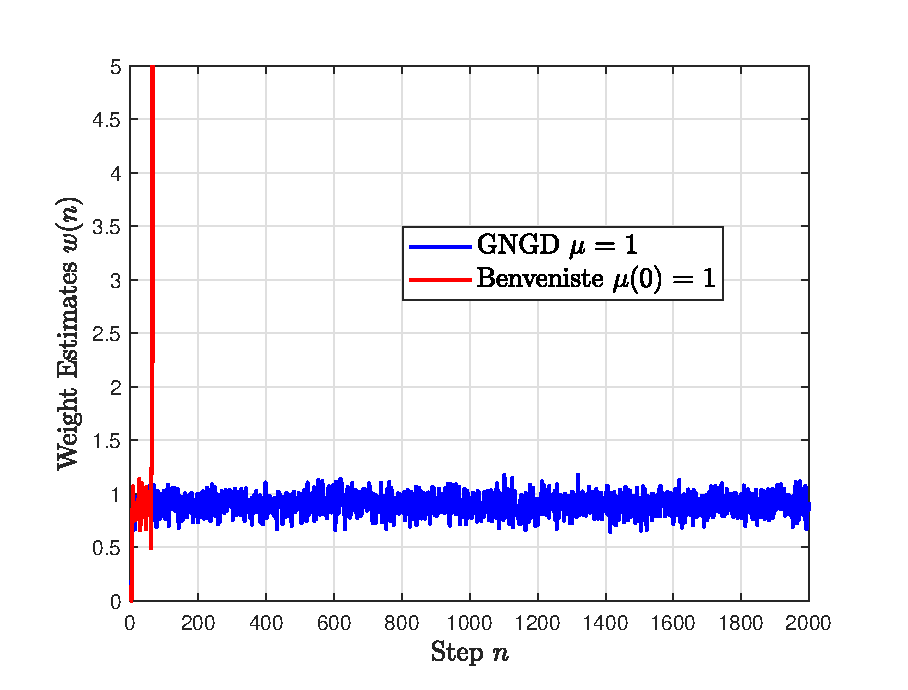
\includegraphics[width=0.48\textwidth]{fig/2.2_4_alter.eps}
        \label{fig14c}
    }
    \caption{Comparison of GNGD algorithm and Benveniste’s algorithm}
    \label{fig14}
\end{figure}

In this part, the GNGD algorithm and Benveniste’s algorithm are compared in identifying the MA(1) system \eqref{eqMA}. 
The value of $\mu$ in GNGD is set to the same value of the initial step size $\mu(0)$ in GASS. 
The value of $\rho$ in GASS is set to $\rho=0.0005$. 

Figure \ref{fig14} shows the weight estimates of MA(1) process in \eqref{eqMA} using different 
$\mu$. We can see that for the small value of $\mu=0.01$, GNGD converges slower than Benveniste’s algorithm but GNGD 
have better performance in steady state error. When $\mu$ increases to $\mu=0.1$, both algorithms 
converge in almost the same speed, but the state error of GNGD is lager. For the very large value of
$\mu$ (i.e., $\mu=1$), the GNGD algorithm can still converge, but Benveniste’s algorithm cannot.


% \begin{figure}[htbp]
%     \centering
% 	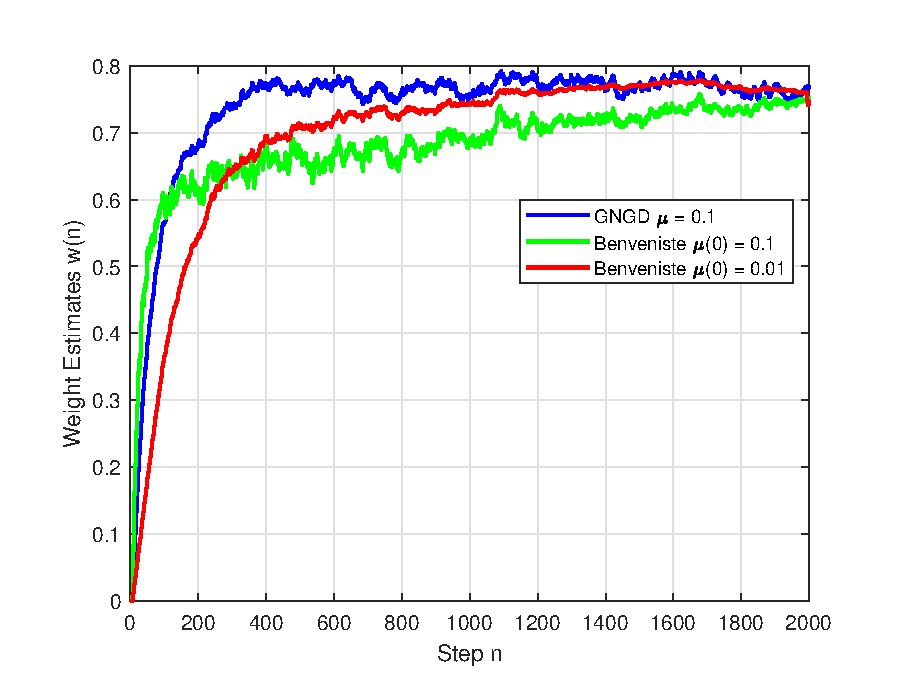
\includegraphics[width=0.48\textwidth]{fig/2.2_3.eps}
%     \caption{Comparison of GNGD and Benveniste’s algorithm}
%     \label{fig14}
% \end{figure}

% Figure \ref{fig14} shows that weight estimates of MA(1) \eqref{eqMA} in GNGD and Benveniste’s algorithms. For GNGD with $\mu=0.1$, it is
% capbale of converging to a similar value as the Benveniste’s algorithm with $\mu=0.01$. The GNGD ($\mu=0.1$) converge faster but has higher steady state error,
% compared with Benveniste’s algorithm ($\mu=0.01$). For Benveniste’s algorithm with $\mu=0.1$, it also converges fast, but the steady state error is much higher than 
% the case of GNGD with $\mu=0.1$.

In terms of complexity, for Benveniste's algorithm, it needs $3M^2+M$ multiplications and $2M^2+M$ additions to
calculate $\psi (n)$, $2M+1$ multiplications and $M+1$ additions to update $\mu(n)$, and $M+1$ multiplications and $M$ additions 
to update ${\bf{w}}(n)$. So there are totally $3M^2 + 4M +2$ multiplications and $2M^2 + 3M + 1$ additions in each step $n$.

Similarly, for GNGD algorithm, it needs $M+6$ multiplications and $2M+2$ additions to update $\epsilon(n)$ as well as 
$2M + 2$ multiplications and $2M + 1$ additions to update ${\bf{w}}(n)$. So, there are totally $3M+8$ multiplications and 
$4M+3$ additions in each step.

As we can see, the computational complexity of Benveniste's algorithm is $O(M^2)$ and that of GNGD is $O(M)$, which 
indicates that the GNGD algorithm has lower computational complexity.

\subsection{Adaptive Noise Cancellation}

\subsubsection{Task a \& b: Adaptive Line Enhancer (ALE)} 
\ \indent
In this part, a noise-corrupted signal is considered, which is given as
\begin{equation}
	s(n) = \sin(0.01\pi n) + \eta(n)
\end{equation}
where $\eta(n)$ is the coloured noise which is given as 
\begin{equation}
	\eta(n) = v(n) + 0.5 v(n-1), \quad v(n) \sim \mathcal{N}(0,1)
\end{equation}
Figure \ref{fig14_14} shows the noised signal
\begin{figure}[htbp]
    \centering
	\includegraphics[width=0.5\textwidth]{fig/2.3_3.pdf}

    \caption{Noise-corrupted signal}
	\label{fig14_14}
\end{figure}

In order to determine the minimum value of delay $\Delta$, we can consider the Mean Square Error 
$\mathbb{E}\{ (s(n) - \hat{x}(n))^2 \}$, from which we can get
\begin{align}
	\mathbb{E}\{ (s(n) - \hat{x}(n))^2 \} & = \mathbb{E}\{ (s(n) - \hat{x}(n)) (s(n) - \hat{x}(n))^T \} \nonumber\\
	& = \mathbb{E}\{ ( s(n) - {\bf{w}}^T(n) {\bf{u}}(n)) ( s(n) - {\bf{u}}^T(n) {\bf{w}}(n)) \} \nonumber\\
	& = \mathbb{E}\{ s(n)^2 \} - 2\mathbb{E}\{ s(n) {\bf{u}}^T(n) \} {\bf{w}}(n) + {\bf{w}}^T(n) \mathbb{E}\{ {\bf{u}}(n) {\bf{u}}^T(n) \} {\bf{w}}(n) \label{eq59}
\end{align}

If the noise in $s(n)$ and ${\bf{u}}(n)$ are uncorrelated, the second term in \eqref{eq59} becomes
\begin{equation}
	- 2\mathbb{E}\{ s(n) {\bf{u}}^T(n) \} {\bf{w}}(n) = -2{\bf{w}}^T(n) \left[ 
		 \begin{matrix}
			 \mathbb{E}\{ x(n) x(n-\Delta) \}\\
			 \vdots\\
			 \mathbb{E}\{ x(n) x(n-\Delta-M+1) \}
		 \end{matrix}
	\right]
\end{equation}
where there is only correlation of the pure signal $x(n)$. Therefore, the linear precoder will minimize the distance 
between the $x(n)$ and $\hat{x}(n)$ in this case. The error $e(n)$ will finally converge to $\eta(n)$ and $\hat{x}(n)$ will converge to
$x(n)$. However, there is noise correlation in $- 2\mathbb{E}\{ s(n) {\bf{u}}^T(n) \} {\bf{w}}(n)$, the coefficients ${\bf{w}}(n)$ will also catch up the
noise, and the both noise and signal will remain in the $e(n)$. Therefore, signal $x(n)$ in $\hat{x}(n)$ will be suppressed.

To ensure the noise in $s(n)$ and ${\bf{u}}(n)$ are uncorrelated, the delay need to be larger than the correlation length of $\eta(n)$,  within which the correlation between the
first and last sample is not zero. According to the expression $\eta(n) = v(n) + 0.5v(n-2)$, its correlation length is 2.
Therefore, we have
\begin{equation}
	\Delta > 2
\end{equation}
The minimum value of delay is 3.


% In the second term $2\mathbb{E}\{ s(n) {\bf{u}}^T(n) \} {\bf{w}}(n)$, there is a corss-correlation $\mathbb{E}\{ s(n) {\bf{u}}^T(n) \}$ \label{eq48}
% between the primary signal and the delayed signal. If the linear predictor minimizes the Mean Square Error, it also
% maximizes the term $2\mathbb{E}\{ s(n) {\bf{u}}^T(n) \} {\bf{w}}(n)$ with respect to ${\bf{w}}(n)$. If there is 
% noise correlation in this term, the linear predictor will also match the noise. Therefore, the noise correlation in this term needs to be 
% removed. By expending this term, we have
% \begin{align}
% 	2\mathbb{E}\{ s(n) {\bf{u}}^T(n) \} {\bf{w}}(n) 
% 	& = 2{\bf{w}}^T(n) \left[ \begin{matrix}
% 		\mathbb{E}\{ s(n) s(n-\Delta) \} \\
% 		\vdots \\
% 		\mathbb{E}\{ s(n) s(n-\Delta-M+1) \} 
% 	\end{matrix} \right] \nonumber\\
% 	& = 2{\bf{w}}^T(n) \left[ \begin{matrix}
% 		\mathbb{E}\{ x(n) x(n-\Delta) \} + \mathbb{E}\{ \eta(n) \eta(n-\Delta) \} \\
% 		\vdots \\
% 		\mathbb{E}\{ x(n) x(n-\Delta-M+1) \} + \mathbb{E}\{ \eta(n) \eta(n-\Delta-M+1) \}  \} 
% 	\end{matrix} \right]  \label{eq49}
% \end{align}
% By observing \eqref{eq49}, we need to choose the $\Delta$ that ensure $\mathbb{E}\{ \eta(n) \eta(n-\Delta - i) \}=0, i=0,...,M-1 $.
% \begin{align}
% 	& \mathbb{E}\{ \eta(n) \eta(n-\Delta - i) \}=0 \nonumber\\
% 	\iff & \mathbb{E}\{ (v(n) + 0.5v(n-2)) (v(n-\Delta - i) + 0.5v(n-\Delta - i-2) \} = 0 \nonumber\\
% 	\iff & \mathbb{E}\{v(n) v(n-\Delta-i) + 0.5 v(n) v(n-\Delta-i-2) + 0.5 v(n-2) v(n-\Delta-i) + 0.25 v(n-2) v(n-\Delta-i-2)\} = 0 \label{eq50}
% \end{align}
% As $v(n)$ is white noise with unit variance, each term in \eqref{eq50} is non-negative and each term needs to be zero. Therefore, we have
% \begin{equation}
% 	\begin{cases}
% 		n-\Delta-i \neq n\\
% 		n-\Delta-i-2 \neq n\\
% 		n-\Delta-i \neq n-2\\
% 		n-\Delta -i-2 \neq n-2\\
% 		\Delta \geq 0\\
% 		M > 1\\
% 		i=0,...,M-1
% 	\end{cases} \iff \Delta > 2 \quad (\text{May be wrong !!!})
% \end{equation}
% The minimum value of the delay $\Delta$ is 3.

% In order to justify the minimum value of the delay calculated above, the following signal is used for test.
% \begin{equation}
% 	s(n) = \sin(0.01\pi n) + \eta (n)
% \end{equation}
% The coefficients ${\bf{w}}(n)$ is updated using LMS algorithm.
Figure \ref{fig15_15} comparison the results of ALE with and without delay. 
One visualize from the figure that the estimated signal is still noise-corrupted if there is 
no delay of the input signal, while the estimated signal is purer when 
$\Delta=3$.

\begin{figure}[htbp]
    \centering
	\subfigure[$\Delta = 0$]{
		\includegraphics[width=0.48\textwidth]{fig/2.3_5.pdf}
        \label{fig15_15a}
	}
    \subfigure[$\Delta = 3$]{
		\includegraphics[width=0.48\textwidth]{fig/2.3_4.pdf}
        \label{fig15_15b}
    }
    \caption{Comparison of different delay}
    \label{fig15_15}
\end{figure}

The MSPE is calculated using ALE with different filter $M$ orders and delays $\Delta$
to investigate the impact of them. The averaged MSPE over 1000 trials is calculated 
for each case. The step size $\mu$ is set to 0.01.

\begin{figure}[H]
    \centering
	\includegraphics[width=0.5\textwidth]{fig/2.3_6.pdf}
	\caption{MSPE against different filter orders and delays}
    \label{fig16_16}
\end{figure}

In Figure \ref{fig16_16}, we can see that the MSPE firstly decreases and then increases 
with the increase of the delay $\Delta$. In terms of filter order, the MSPE dropped sharply 
when the order changed from 5 to 10. Nevertheless, as the order changes from 10 to 15 or 20,
there is no significant drop of MSPE and it even increases sometimes. Given the
computational cost increase with $M$, the best choice is $M=10$.


\subsubsection{Task c: Adaptive Noise Cancellation (ANC)}
\ \indent
In this part, the ANC is implemented to compare with ALE, where the filter order $M$ and 
step size $\mu$ are set to 10 and 0.01, respectively. The result is shown in Figure \ref{fig17_17}.

\begin{figure}[htbp]
    \centering
	\includegraphics[width=0.5\textwidth]{fig/2.3_7.pdf}
	\caption{Noiseless signal and estimated signal by ANC}
    \label{fig17_17}
\end{figure}
The MSPE in this case is 0.0038. For ALE, the minimum MSPE for $M=10$ is achieved when $\Delta=6$, which is 0.065. 
Therefore, the ANC outperforms ALE in de-nosing the noisy sinusoid signal.

\subsubsection{Task d: Denoise EEG Data}
\ \indent
In the EEG data, there is a strong 50Hz component introduce by the mains. Figure \ref{fig15a} shows the 
spectrum of the corrupted EEG data using $\mathtt{spectrogram}$ function with window length of 
1000 and overlap of 500. There is a bright yellow vertical line at 50Hz in this figure, which represents for the 
noise.

The ANC is exploited to suppress the 50Hz component in EEG data. The reference noise signal is genereated 
according to 
\begin{equation}
	r(n) = sin(2\pi\times 50 \times T_s \times n) + w(n)
\end{equation}
where $T_s$ is the sampling interval and $w(n) \sim \mathcal{N}(0,1)$ is the white Gaussian noise.
The sampling frequency of EEG data is $f_s = 1200$Hz, so $T_s = 1/f_s = 1/1200$s. 
In ANC, the step size is set to $\mu=0.01$ and the filter length is set to $M=15$. 

Figure \ref{fig15b} shows the spectrum of the EEG data denoised by ANC, where we can see that the bright yellow line at $50$Hz 
in Figure \ref{fig15a} disappears and other frequency components are not affected. Therefore, the noise 
introduced by the mains is almost totally removed.


\begin{figure}[H]
    \centering
	\subfigure[Corrupted]{
		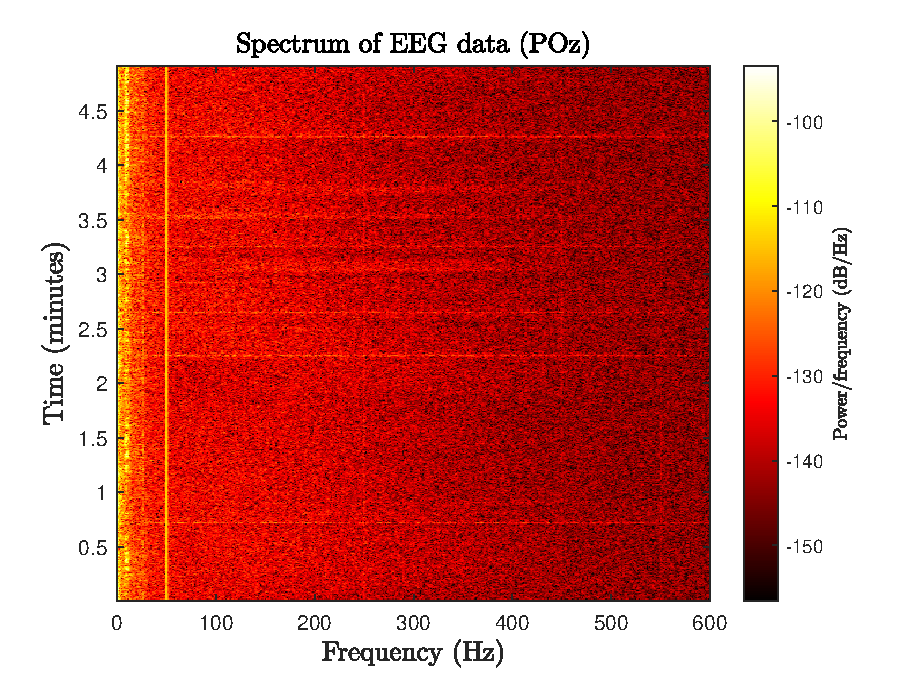
\includegraphics[width=0.48\textwidth]{fig/2.3_1.eps}
        \label{fig15a}
	}
    \subfigure[Denoised]{
		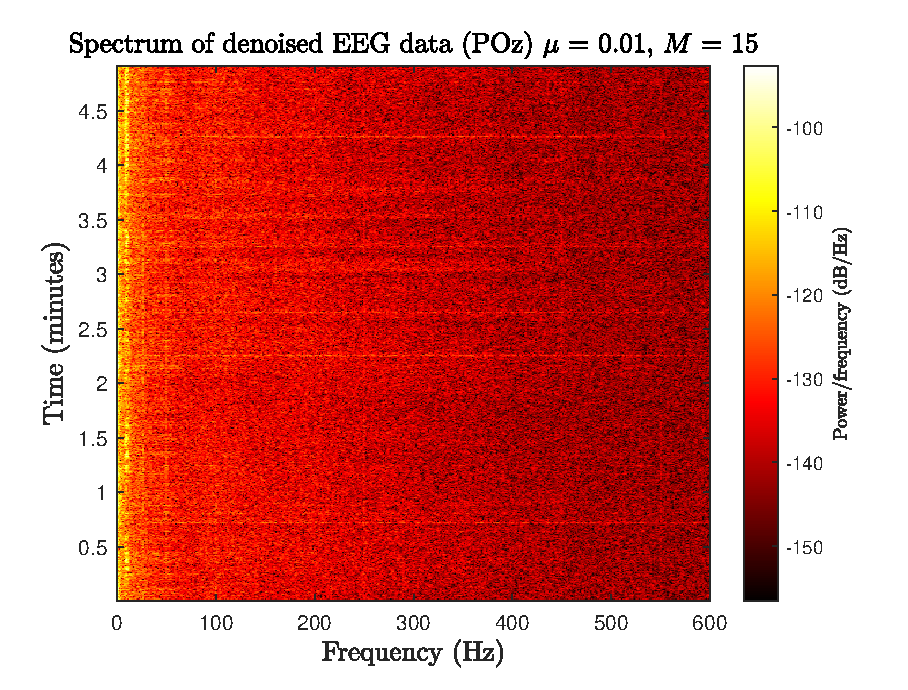
\includegraphics[width=0.48\textwidth]{fig/2.3_2.eps}
        \label{fig15b}
    }
    \caption{Spectrum of corrupted and denoised EEG data}
    \label{fig15}
\end{figure}

\newpage
\section{Widely Linear Filtering and Adaptive Spectrum Estimation}

\subsection{Complex LMS and Widely Linear Modelling}

\subsubsection{Task a: Comparison of CLMS and ACLMS}
\ \indent
In the complex LMS (CMLS) algorithm, the weights update procedure is given as 
\begin{align}
	\hat{y}(n) & = {\bf{h}}^H(n) {\bf{x}}(n) \nonumber\\
	e(n) & = y(n) - \hat{y}(n) \\
	{\bf{h}}(n+1) & = {\bf{h}}(n) + \mu e^*(n) {\bf{x}}(n) \nonumber
\end{align}
In the argumented CLMS (ACLMS) algorithm, the procedure is given as 
\begin{align}
	\hat{y}(n) & = {\bf{h}}^H(n) {\bf{x}}(n) + {\bf{g}}^H(n) {\bf{x}}^*(n) \nonumber\\
	e(n) & = y(n) - \hat{y}(n) \\
	{\bf{h}}(n+1) & = {\bf{h}}(n) + \mu e^*(n) {\bf{x}}(n) \nonumber\\
	{\bf{g}}(n+1) & = {\bf{g}}(n) + \mu e^*(n) {\bf{x}}^*(n) \nonumber
\end{align}

To compare CLMS and ACLMS, a WLMA(1) process is considered, which is given as
\begin{equation}
	y(n) = x(n) + b_1 x(n-1) + b_2 x^*(n-1), \quad x \sim {\mathcal{CN}}(0,1)
\end{equation}
where $b_1 = 1.5 + 1j$ and $b_2 = 2.5 - 0.5j$. Both CLMS and ACLMS algorithms are
implemented in the system identification setting to identify the WLAM model. The 
input to the model and CLMS/ACLMS is ${\bf{x}}(n) = [x(n-1)]^T$.

Figure \ref{fig16} shows the leaning curves, $10\log_{10} |e(n)|^2$, of CLMS and ACLMS by
averaging the results of 100 trials. For CLMS, the square error $|e(n)|^2$ is always 
around 7dB. However, for the ACLMS, its square error finally converges to around -3dB, which is much 
lower than that in CLMS. Therefore, ACLMS have better performance in terms of steady
state error when learning the weights of WLMA(1) model.

\begin{figure}[htbp]
    \centering
	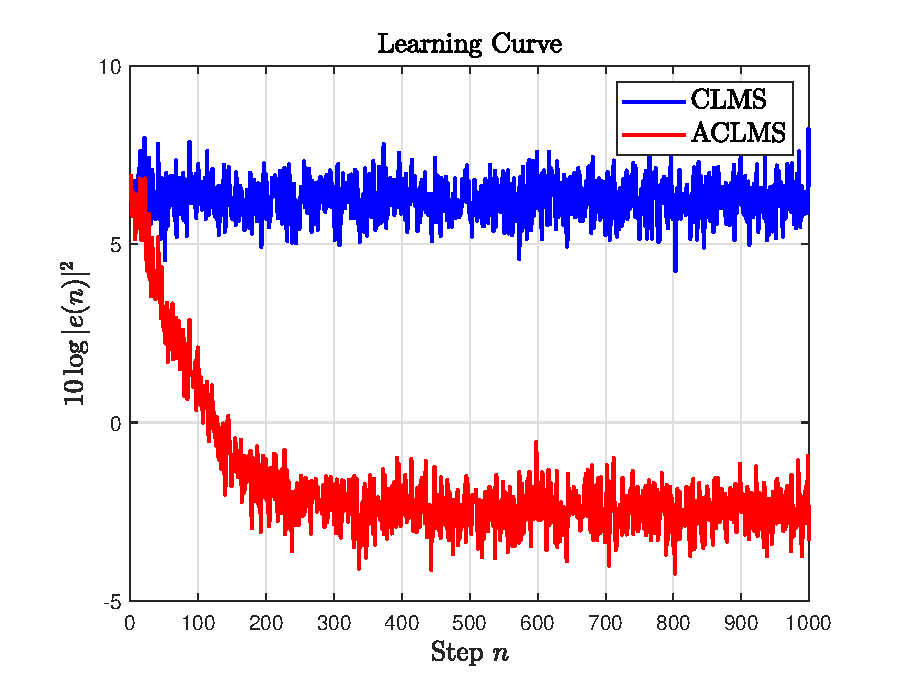
\includegraphics[width=0.48\textwidth]{fig/3.1_1.eps}
    \caption{Learning curves of CLMS and ACLMS}
    \label{fig16}
\end{figure}

\subsubsection{Task b: Processing Wind Data}
\ \indent
Figure \ref{fig17} shows the scatter diagrams of wind data. Based on observation, the 
three complex wind signals are all non-circular, because the properties of 
signals would be changes if they are rotated. Their circularity can also be 
analysed quantitatively using circularity coefficient, which is defined as 
\begin{equation}
	|\rho| = \frac{|p|}{c}, \quad c = \mathbb{E}\{ z z^* \}, \quad p = \mathbb{E}\{ z z^T \} \label{eq61}
\end{equation}
where $c$ and $p$ are the covariance and pseudocovariance of $z$, respectively. In practice, 
they can be approximated by 
\begin{equation}
	c = \frac{1}{N} {\bf{z}}^H {\bf{z}}, \quad p = \frac{1}{N} {\bf{z}}^T {\bf{z}} \label{eq62}
\end{equation}
where $N$ is the number of data samples and $z = [z(0),...,z(N-1)]^T$. The circularity coefficients 
of the low, medium and high wind data is calculated based on \eqref{eq61} and \eqref{eq62}.
\begin{align}
	\text{low}:& \quad|\rho_l| = 0.1592 \nonumber\\
	\text{medium}:& \quad|\rho_m| = 0.4543 \label{eq63} \\ 
	\text{high}:& \quad|\rho_h| = 0.6237 \nonumber 
\end{align}
According to circularity coefficients in \eqref{eq63}, the circularity of low wind signal is highest and
that of high wind data is lowest.

\begin{figure}[htbp]
    \centering
	\subfigure[Low wind]{
		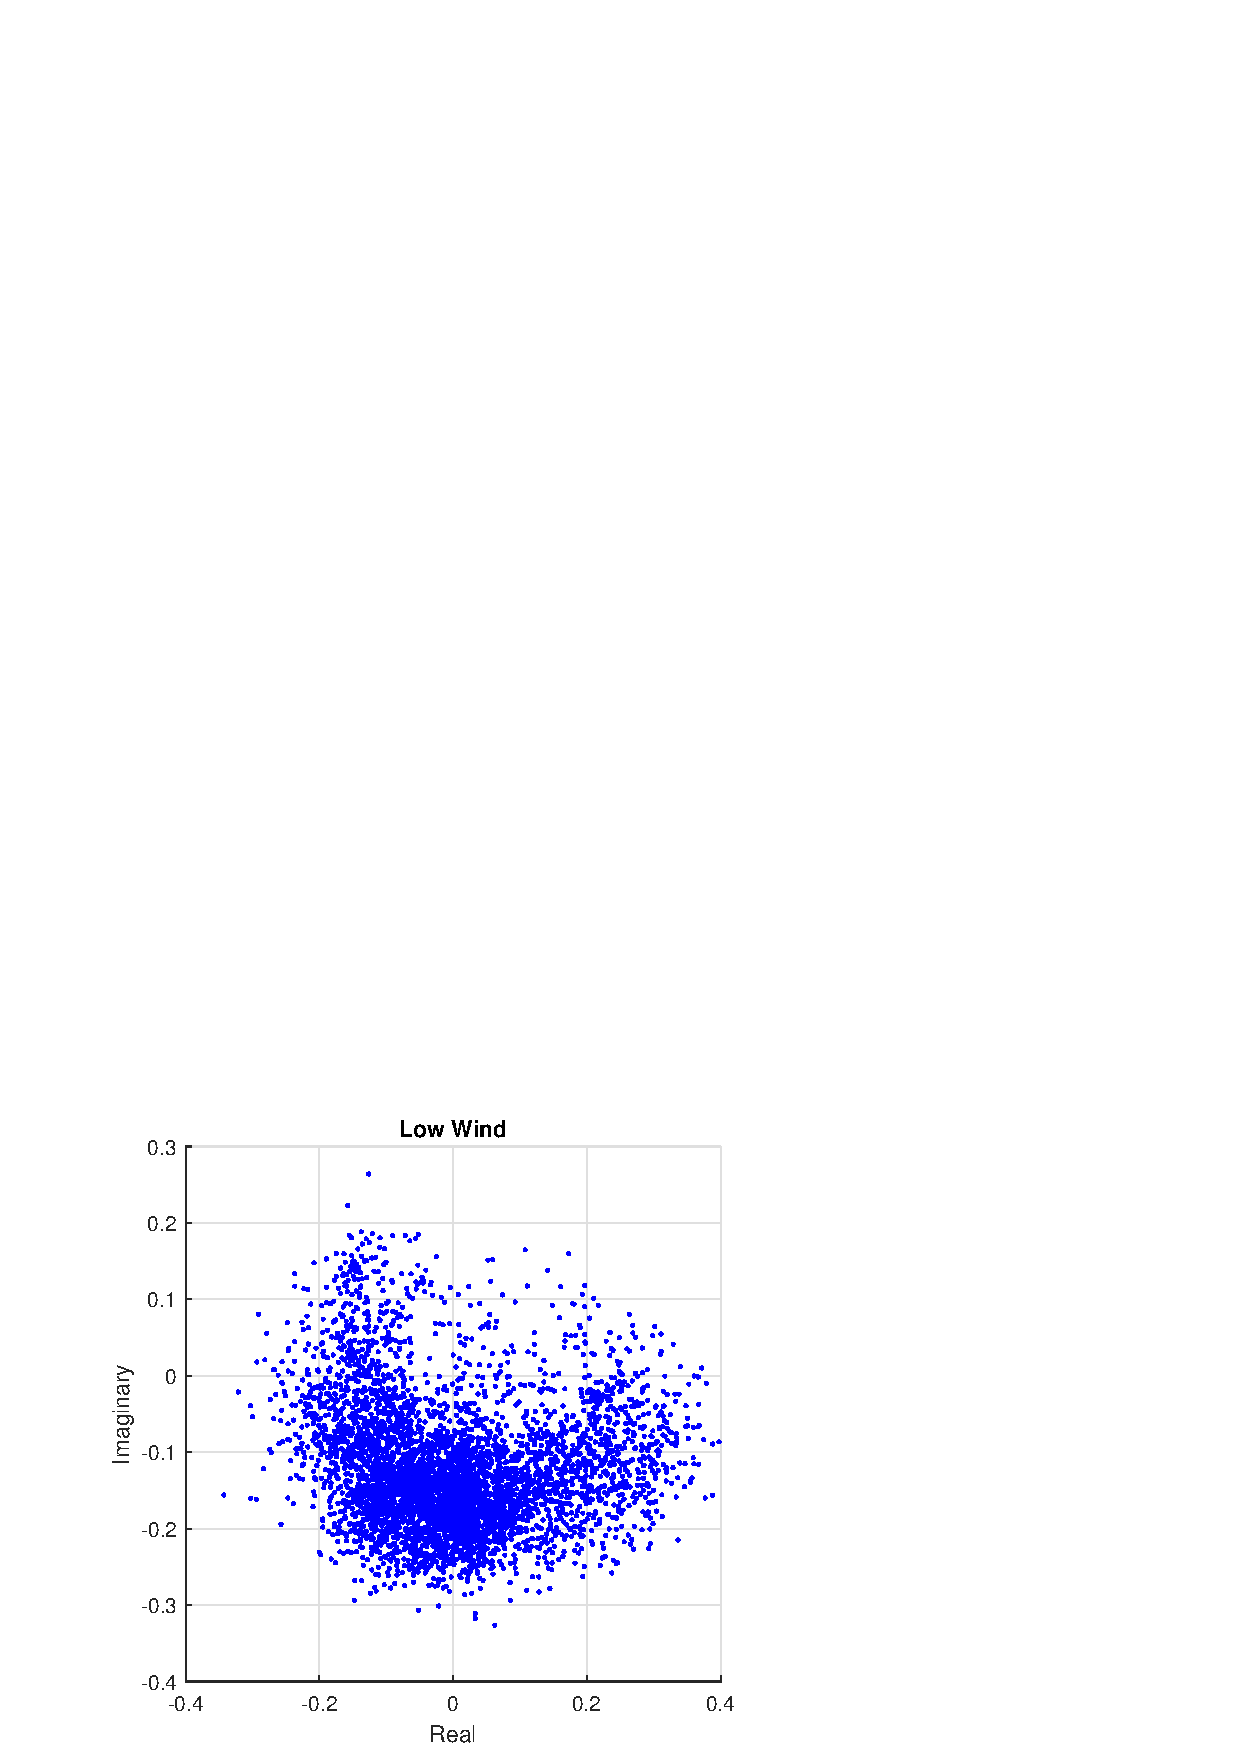
\includegraphics[width=0.31\textwidth]{fig/3.1_2.pdf}
        \label{fig17a}
	}
    \subfigure[Medium wind]{
		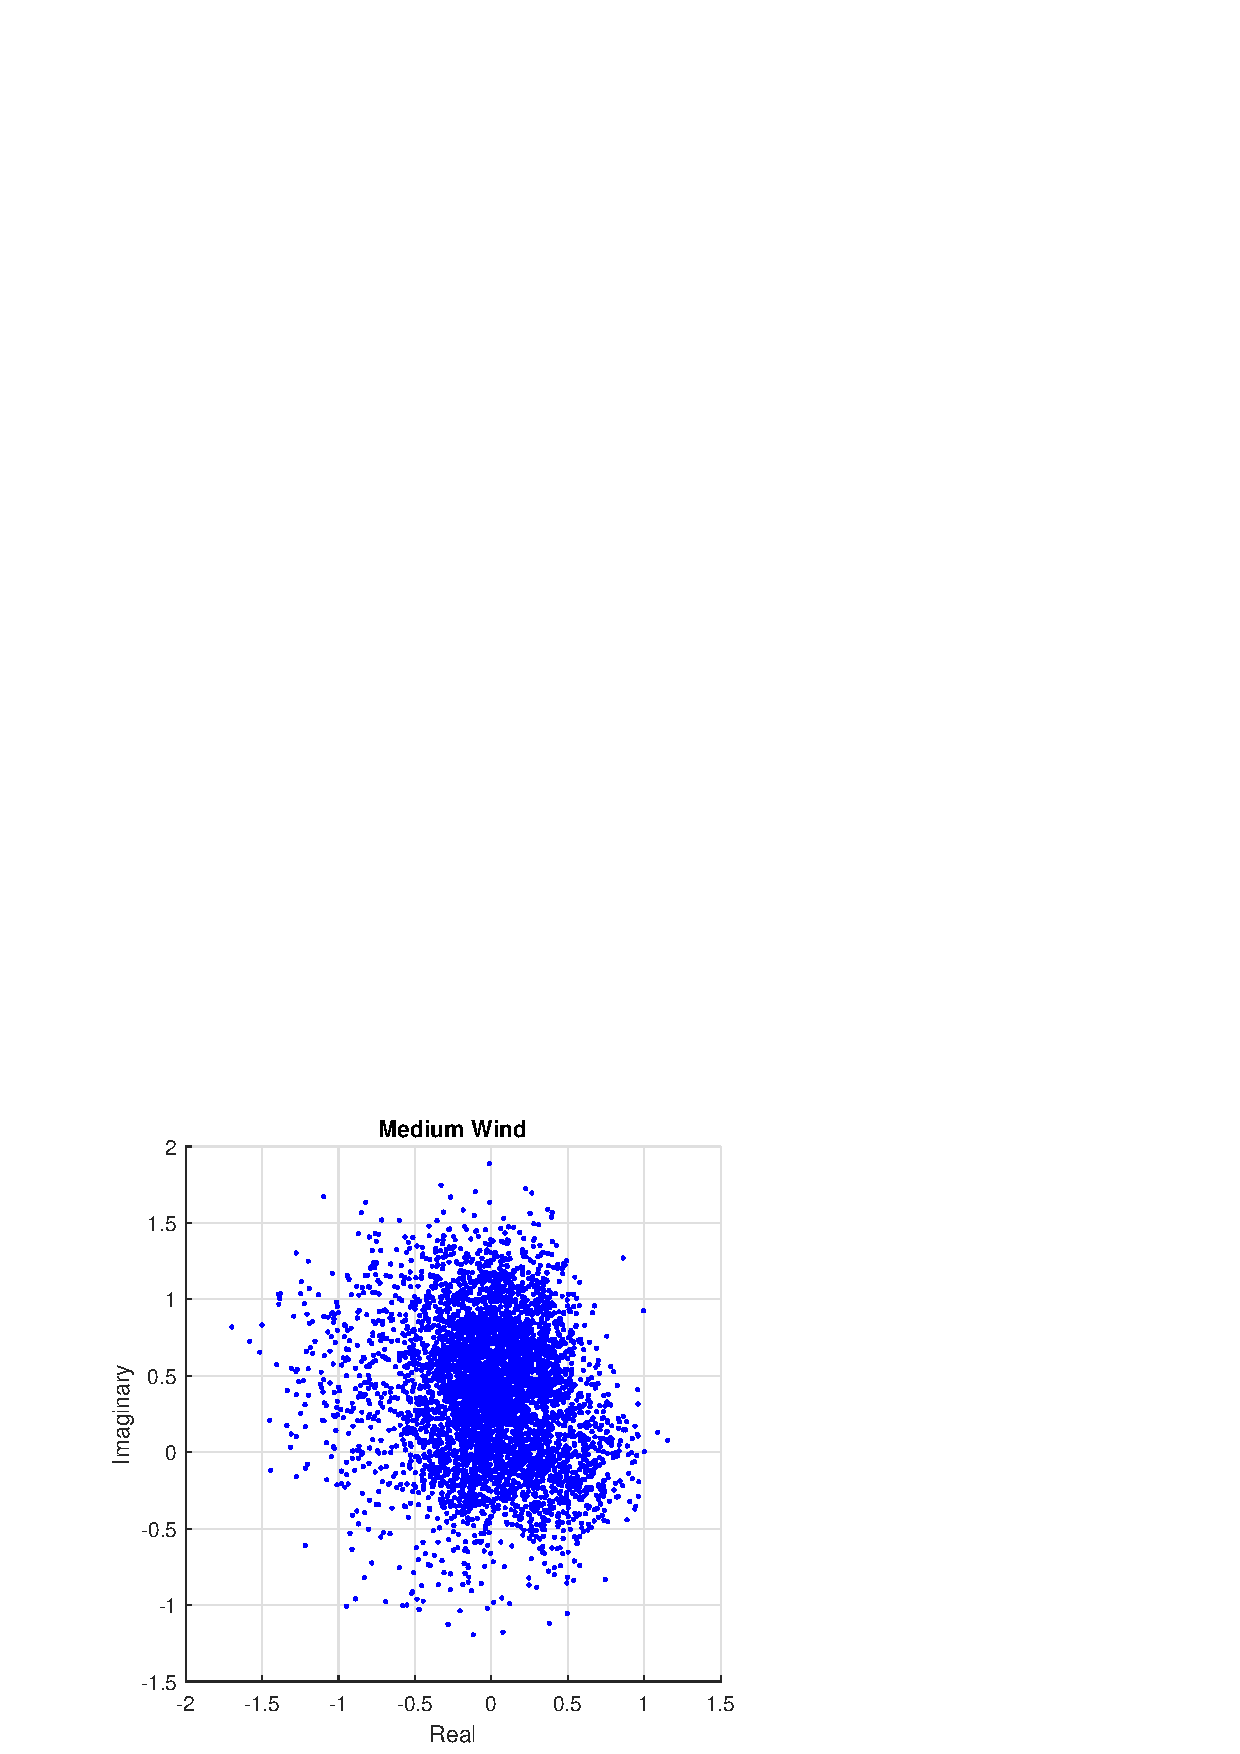
\includegraphics[width=0.31\textwidth]{fig/3.1_3.pdf}
        \label{fig17b}
    }
	\subfigure[High wind]{
		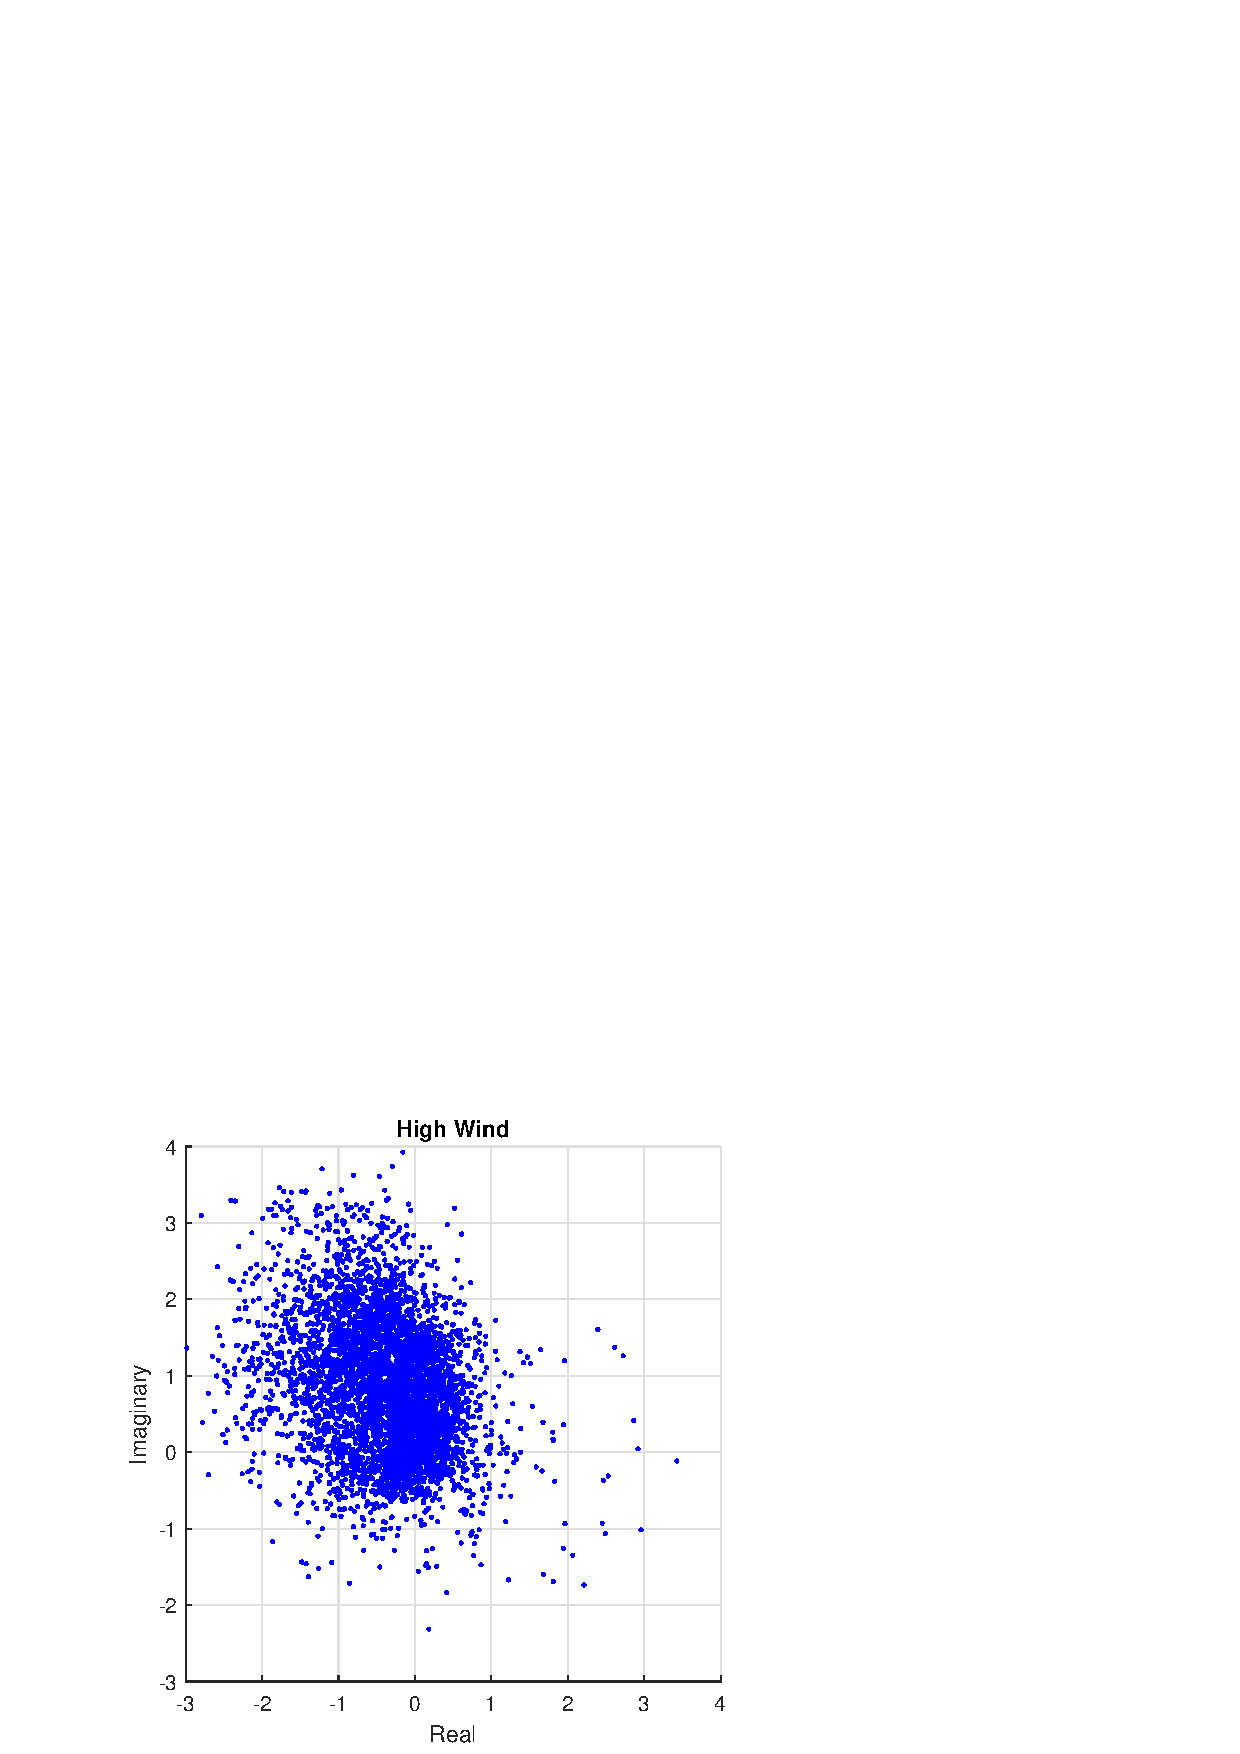
\includegraphics[width=0.31\textwidth]{fig/3.1_4.pdf}
        \label{fig17b}
    }
    \caption{Scatter diagrams of wind data}
    \label{fig17}
\end{figure}

The CLMS and ACLMS filter are configured in a prediction setting to perform a one-step ahead 
prediction, i.e., using the past wind data to predict one future win data. The wind signals 
in east-west and north-south directions are firstly combined to a complex signal
\begin{equation}
	v(n) = v_{\text{east}}(n) + j v_{\text{north}}(n)
\end{equation}
The signal input to the CLMS and ACLMS is ${\bf{x}}(n) = [v(n-1),...,v(n-M)]^T$, which is used to
predict $v(n)$. The prediction gain $R_p$ is exploited to evaluate the performance of CLMS and ACLMS.
The prediction gain is defined as
\begin{equation}
	R_p = 10 \log_{10} \frac{\sigma_v^2}{\sigma_e^2}
\end{equation}
where $\sigma_v^2 = \mathbb{E} \left\{ |v(n)|^2 \right\}$ is the signal power and $\sigma_e^2 = \mathbb{E} \left\{ |e(n)|^2 \right\}$ is the error power.

\begin{figure}[htbp]
    \centering
	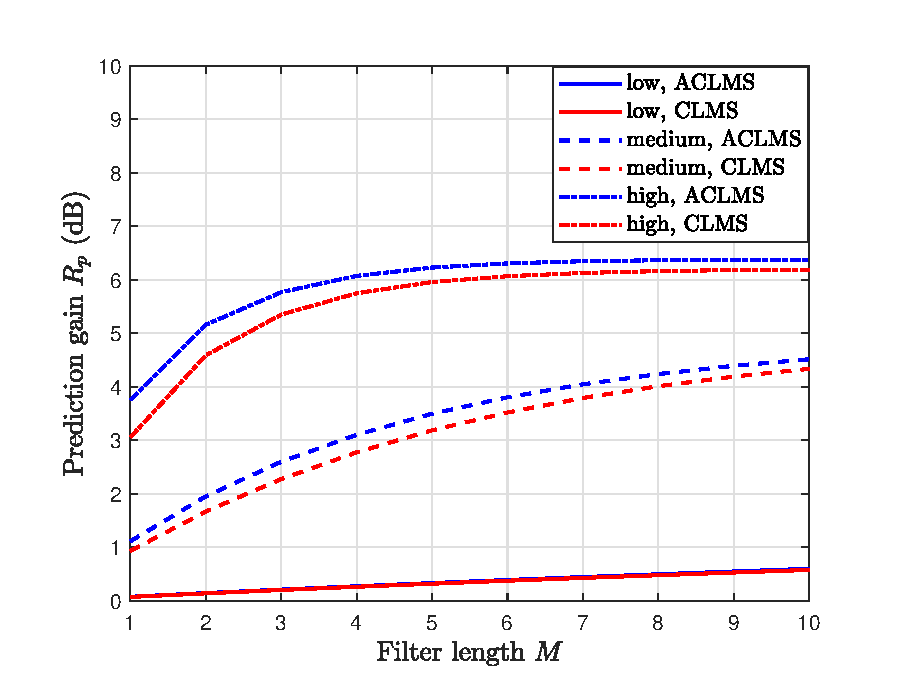
\includegraphics[width=0.48\textwidth]{fig/3.1_5.eps}
    \caption{Comparison of CLMS and ACLMS for different wind regimes}
    \label{fig18}
\end{figure}

Figure \ref{fig18} evaluates CLMS and ACLMS in terms of prediction gain. For the 
low wind signal, which has high circularity, CLMS and ACLMS has almost the same performance.
For the wind signals that have low circularity (i.e., medium and high wind), the ACLMS outperforms the 
CLMS algorithm. 

\subsubsection{Task c: Circularity Diagrams of Complex $\alpha$-$\beta$ Voltages}
\ \indent
In this section, the balanced and unbalanced three-phase voltages are generated with 
system frequency $f_o=50$Hz and sampling frequency $f_s=1000$Hz.

Figure \ref{fig19} shows the circularity diagram of balanced system, where all the voltages locate 
at several points which make up a circle. The amplitude of all the complex voltages are the same. 
Therefore, the balanced complex voltages have very high circularity.
When the phase $\phi$ is changed, the points rotate angle of $\phi$ around the origin in counterclockwise. 

Figure \ref{fig20} shows the circularity diagram of unbalanced systems with $f_o=50$Hz, $f_s=1000$Hz and $\phi=0$. 
The magnitudes ($V_b, V_c$) and phases ($\Delta_b, \Delta_c$) are changed to explore their impact.
In the unbalanced systems, all the voltages also locate at several points, but these points 
become non-circular, which can be a criterion to identify whether there is a fault. 

\begin{figure}[htbp]
    \centering
	\subfigure{
		\includegraphics[width=0.31\textwidth]{fig/3.1_6.pdf}
	}
    \subfigure{
		\includegraphics[width=0.31\textwidth]{fig/3.1_7.pdf}
    }
	\subfigure{
		\includegraphics[width=0.31\textwidth]{fig/3.1_8.pdf}
    }
    \caption{Circularity diagrams balanced complex voltages}
    \label{fig19}
\end{figure}

\begin{figure}[htbp]
    \centering
	\subfigure{
		\includegraphics[width=0.23\textwidth]{fig/3.1_9.pdf}
    }
	\subfigure{
		\includegraphics[width=0.23\textwidth]{fig/3.1_10.pdf}
    }
	\subfigure{
		\includegraphics[width=0.23\textwidth]{fig/3.1_11.pdf}
    }
	\subfigure{
		\includegraphics[width=0.23\textwidth]{fig/3.1_12.pdf}
    }
	\subfigure{
		\includegraphics[width=0.23\textwidth]{fig/3.1_13.pdf}
    }
	\subfigure{
		\includegraphics[width=0.23\textwidth]{fig/3.1_14.pdf}
    }
	\subfigure{
		\includegraphics[width=0.23\textwidth]{fig/3.1_15.pdf}
    }
	\subfigure{
		\includegraphics[width=0.23\textwidth]{fig/3.1_16.pdf}
    }
    \caption{Circularity diagrams unbalanced complex voltages with different magnitudes and phases (blue points are "unbalanced"; red points are "balanced")}
    \label{fig20}
\end{figure}

\subsubsection{Task d \& e: Estimates of System Frequency}
\ \indent
Consider the strictly linear autoregressive model, given by
\begin{equation}
	v(n+1) = h^*(n)v(n) \label{eq66}
\end{equation}
The frequency of balanced complex $\alpha$-$\beta$ voltage can be expressed as 
\begin{equation}
	f_o(n) = \frac{f_s}{2\pi} \arctan \left\{ \frac{\mathfrak{I}\{ h(n) \}}{\mathfrak{R}\{ h(n) \}} \right\} \label{eq67}
\end{equation}

\begin{proof}
	In balanced system, the complex voltage is expressed as
	\begin{equation}
		v(n) = \sqrt{ \frac{3}{2} } V e^{ j \left( 2\pi \frac{f_o}{f_s} n + \phi \right) }
	\end{equation}
	According to \eqref{eq66}, we have
	\begin{gather}
		h^*(n)  = \frac{\sqrt{ \frac{3}{2} } V e^{ j \left( 2\pi \frac{f_o}{f_s} (n+1) + \phi \right) }}{\sqrt{ \frac{3}{2} } V e^{ j \left( 2\pi \frac{f_o}{f_s} n + \phi \right) }} \\
		h^*(n)  = e^{j 2\pi \frac{f_o}{f_s}} \label{eq70}
	\end{gather}
	The two side of \eqref{eq70} must be co-phased. According to Nyquist sampling 
	theory, we must have $0 < 2\pi \frac{f_o}{f_s} \leq \pi \quad ( f_s \geq 2 f_o )$.
	Therefore, we have
	\begin{gather}
		2 \pi \frac{f_o}{f_s} = \arctan \left\{  \frac{\mathfrak{I}\{ h(n) \}}{\mathfrak{R}\{ h(n) \}} \right\} \\
		f_o = \frac{f_s}{2 \pi} \arctan \left\{  \frac{\mathfrak{I}\{ h(n) \}}{\mathfrak{R}\{ h(n) \}} \right\}
	\end{gather}
	$\hfill\blacksquare$ 
\end{proof}

Similarly, if we consider the following widely linear autoregressive model 
\begin{equation}
	v(n+1) = h^*(n) v(n) + g^*(n) v^*(n) \label{eq73}
\end{equation}
the frequency of unbalanced voltage is 
\begin{equation}
	f_o(n) = \frac{f_s}{2\pi} \arctan \left\{  \frac{ \sqrt{\mathfrak{I}^2\{ h(n) \} - |g(n)|^2 } }{\mathfrak{R}\{ h(n) \}} \right\} \label{eq74}
\end{equation}

\begin{proof}
	In unbalanced system, the complex voltage is given as 
	\begin{equation}
		v(n) = A e^{ j \left( 2\pi \frac{f_o}{f_s} n + \phi \right) } + B e^{ -j \left( 2\pi \frac{f_o}{f_s} n + \phi \right) }
	\end{equation}
	According to \eqref{eq73}, we have the following equivalent equations.
	\begin{align}
		g^*(n) &= \frac{v(n+1) - h^*(n)v(n)}{v^*(n)} \\
		g(n) g^*(n) &= \frac{\Bigl(v(n+1) - h^*(n)v(n)\Bigl) \Bigl(v^*(n+1) - h(n)v^*(n)\Bigl)}{v(n) v^*(n)} \\
		|g(n)|^2 &= \frac{v(n+1) v^*(n+1)}{v(n) v^*(n)} - \frac{h(n) v(n+1)}{v(n)} - \frac{h^*(n) v^*(n+1)}{v^*(n)} + h(n)h^*(n) \\
		|g(n)|^2 &= \left( e^{ j 2\pi \frac{f_o}{f_s} } \right)^2 - (h(n) + h^*(n))e^{ j 2\pi \frac{f_o}{f_s} } + |h(n)|^2 \\
		|g(n)|^2 &= \left( e^{ j 2\pi \frac{f_o}{f_s} } \right)^2 - 2 \mathfrak{R}\{ h(n) \} e^{ j 2\pi \frac{f_o}{f_s} } + \mathfrak{R}^2\{ h(n) \} + \mathfrak{I}^2\{ h(n) \} \\
		|g(n)|^2 - \mathfrak{I}^2\{ h(n) \} &= \left( e^{ j 2\pi \frac{f_o}{f_s} } - \mathfrak{R}\{ h(n) \} \right)^2 \\
		j \sqrt{ \mathfrak{I}^2\{ h(n) \} - |g(n)|^2 } &= e^{ j 2\pi \frac{f_o}{f_s} } - \mathfrak{R}\{ h(n) \} \\
		e^{ j 2\pi \frac{f_o}{f_s} } &= \mathfrak{R}\{ h(n) \} + j \sqrt{ \mathfrak{I}^2\{ h(n) \} - |g(n)|^2 }
	\end{align}
	\begin{align}
		2\pi \frac{f_o}{f_s} &= \arctan \left\{ \frac{ \sqrt{ \mathfrak{I}^2\{ h(n) \} - |g(n)|^2 } }{ \mathfrak{R}\{ h(n) \} } \right\} \\
		f_o &= \frac{f_s}{2\pi} \arctan \left\{ \frac{ \sqrt{ \mathfrak{I}^2\{ h(n) \} - |g(n)|^2 } }{ \mathfrak{R}\{ h(n) \} } \right\}
	\end{align}
	$\hfill\blacksquare$ 
\end{proof}

Therefore, based on \eqref{eq66}, \eqref{eq67}, \eqref{eq73} and \eqref{eq74}, we can use CLMS and ACLMS
to estimate the frequency of balanced and unbalanced system. The parameters of balanced
system and unbalanced system are shown below. 

\begin{table}[htbp]
	\caption{Parameters of balanced and unbalanced systems}
	\centering
    \setlength{\tabcolsep}{4mm}{
        \centering
        \begin{tabular}{ccc}% 通过添加 | 来表示是否需要绘制竖线
            \toprule
             &Balanced & Unbalanced\\\hline
			$f_o$ & 50Hz & 50Hz\\

			$f_s$ & 1000Hz & 1000Hz \\

            $V_a$ & 1 & 1\\

            $V_b$ & 1 & 1\\

            $V_c$ & 1 & 2\\

			$\phi$ & 0 & 0\\

			$\Delta_b$ & 0 & 0\\

			$\Delta_c$ & 0 & $\frac{1}{3}\pi$\\

            \bottomrule
        \end{tabular} \label{table5}
    }
\end{table}

Figure \ref{fig21} shows the frequency estimates for balanced and unbalanced systems.
For the balanced system, the CLMS algorithm is capable of getting the correct frequency 
from the first step and the ACLMS algorithm can also converge to the correct frequency
after several steps. For the unbalanced system, the ACMLS can estimate the frequency correctly.
However, the CLMS algorithm cannot converge to the correct frequency. The main reason is that
the complex voltages of unbalanced system are non-circular, on which the CLMS performs bad 
because of the conjugate component. 

\begin{figure}[htbp]
    \centering
	\subfigure[Balanced]{
		\includegraphics[width=0.48\textwidth]{fig/3.1_17.eps}
	}
    \subfigure[Unbalanced]{
		\includegraphics[width=0.48\textwidth]{fig/3.1_18.eps}
    }
    \caption{Comparison of CLMS and ACLMS for frequency estimation}
    \label{fig21}
\end{figure}

\subsection{Adaptive AR Model Based Time-Frequency Estimation} \label{part3.2}
\ \indent
The conventional AR model can only estimate the spectrum of stationary signals. 
In this part, the adaptive AR model is investigated to estimate the non-stationary
signal.

The following frequency modulated signal is considered.
\begin{equation}
	y(n) = e^{j \left( \frac{2\pi}{f_s} \phi(n) \right)} + \eta(n) \label{eq86}
\end{equation}
where $\eta(n) \sim \mathcal{CN} (0,0.05)$ and $\phi(n) = \int f(n) dn $. 
$f(n)$ is a frequency signal which is given as
\begin{equation}
	f(n) = \begin{cases}
		100, &1 \leq n \leq 500\\
		100 + \frac{n-500}{2}, &501 \leq n \leq 1000 \\
		100 + \left( \frac{n-1000}{25} \right)^2, &1001 \leq n \leq 1500
	\end{cases}
\end{equation}
Figure \ref{fig22} shows the plot of $f(n)$. As the maximal frequency is $500$Hz,
the sample frequency is set to $f_s=1000$Hz.

\begin{figure}[htbp]
    \centering
	\includegraphics[width=0.5\textwidth]{fig/3.2_1.pdf}

    \caption{Frequency signal $f(n)$}
    \label{fig22}
\end{figure}

The conventional AR(1) model is firstly used to estimate the spectrum of $y(n)$.
The MATLAB function $\mathtt{aryule}$ is used to calculate the AR(1) coefficient and
the function $\mathtt{freqz}$ is used to calculated the spectrum.

Figure \ref{fig23} shows the spectrum estimated by the AR(1) model. Obviously, 
this method cannot capture the changes of frequency in $f(n)$.

\begin{figure}[htbp]
    \centering
	\includegraphics[width=0.5\textwidth]{fig/3.2_2.pdf}

    \caption{Spectrum estimated by AR(1) model}
    \label{fig23}
\end{figure}

In order to capture the frequency changes, we can use the adaptive AR(1) model, where 
the CLMS algorithm is exploited to estimate the time-frequency spectrum. The adaptive AR(1)
model follows \eqref{eq66}.

\begin{figure}[htbp]
    \centering
	\includegraphics[width=0.6\textwidth]{fig/3.2_3.png}

    \caption{Time-frequency spectrum estimated by adaptive AR(1) model}
    \label{fig24}
\end{figure}

Figure \ref{fig24} shows the time-frequency estimated by adaptive AR(1) model.
The bright parts in this figure represent the frequency components. We can see that 
the time-varying frequencies match the plot of frequency $f(n)$ in Figure \ref{fig22}.
Therefore, the CLMS-based adaptive AR model is capable of estimating the frequency of 
a non-stationary signal, while the conventional AR spectrum is only suitable for stationary signal.

\subsection{A Real Time Spectrum Analyser Using Least Mean Square}

\subsubsection{Task a \& b: Least Squares Solution and Discrete Fourier Transform}
\ \indent
Consider the signal $\hat{\bf{y}} = {\bf{Fw}}$, which is an estimate of the actual signal 
${\bf{y}}$. The matrix ${\bf{F}}$ is given as 
\begin{equation}
	{\bf{F}} = \left[ \begin{matrix}
		1 & 1 & \cdots & 1\\
		1 & e^{j \frac{2\pi}{N}(1)(1)} & \cdots & e^{j \frac{2\pi}{N}(1)(N-1)}\\
		\vdots & \vdots & \ddots & \vdots \\
		1 & e^{j \frac{2\pi}{N}(N-1)(1)} & \cdots & e^{j \frac{2\pi}{N}(N-1)(N-1)}
	\end{matrix} \right] \label{eq89}
\end{equation}

The least squares problem is solved by minimising the cost function
\begin{equation}
	\min_{\bf{w}} \Vert {\bf{y}} - \hat{\bf{y}} \Vert^2 \label{eq88}
\end{equation}
The solution of problem \eqref{eq88} is given as
\begin{equation}
	{\bf{w}} = \left( {\bf{F}}^H{\bf{F}} \right)^{-1} {\bf{F}}^H {\bf{y}} \label{eq89}
\end{equation}

\begin{proof}
	By expending the \eqref{eq88}, we have
	\begin{align}
		\Vert {\bf{y}} - \hat{\bf{y}} \Vert^2 & = ( {\bf{y}} - \hat{\bf{y}} )^H( {\bf{y}} - \hat{\bf{y}} ) \nonumber \\
		& = ( {\bf{y}} - {\bf{F}} {\bf{w}} )^H( {\bf{y}} - {\bf{F}} {\bf{w}} ) \nonumber \\
		& = {\bf{w}}^H {\bf{F}}^H {\bf{F}} {\bf{w}} - 2 {\bf{F}}^H {\bf{y}} {\bf{w}} + {\bf{y}}^H {\bf{y}} \label{eq90}
	\end{align}
	It is obvious that ${\bf{F}}^H {\bf{F}}$ is a semi-definite matrix, so the problem \eqref{eq88} is 
	an unconstrained convex optimization problem, the solution of which is given by 
	$\frac{\partial{ \Vert {\bf{y}} - \hat{\bf{y}} \Vert^2 }}{ \partial{\bf{w}}} = 0$.
	Based on \eqref{eq90}, we have
	\begin{align}
		\frac{\partial{ \Vert {\bf{y}} - \hat{\bf{y}} \Vert^2 }}{ \partial{\bf{w}}} & = ({\bf{F}}^H {\bf{F}} + {\bf{F}} {\bf{F}}^H) {\bf{w}} - 2{\bf{F}}^H {\bf{y}} \nonumber\\
		& = 2{\bf{F}}^H {\bf{F}} {\bf{w}} - 2{\bf{y}}{\bf{F}} \label{eq90}
	\end{align}
	By setting \eqref{eq90} to zero, we have
	\begin{gather}
		2{\bf{F}}^H {\bf{F}} {\bf{w}} - 2{\bf{F}}^H{\bf{y}} = 0 \\
		{\bf{F}}^H {\bf{F}} {\bf{w}} = {\bf{F}}^H{\bf{y}} \\
		{\bf{w}} = \left( {\bf{F}}^H{\bf{F}} \right)^{-1} {\bf{F}}^H {\bf{y}}
	\end{gather}

	$\hfill\blacksquare$ 
\end{proof}

The solution \eqref{eq89} has a strong relationship with the discrete Fourier transform (DFT).
Denote the DFT of ${\bf{y}}$ by ${\bf{d}} = [d(0),...,d(N-1)]^T$. 
\begin{equation}
	y(n) = \frac{1}{N} \sum_{k=0}^{N-1} d(k) e^{ j \frac{2\pi}{N} n k }, \quad n=0,...,N-1 \label{eq96}
\end{equation}
Observing the structure of matrix ${\bf{F}}$ and equation \eqref{eq96}, ${\bf{y}}$ can be rewritten as
\begin{equation}
	{\bf{y}} = \frac{1}{N} {\bf{F}} {\bf{d}}
\end{equation}
Substitute it into equation \eqref{eq89}, we have
\begin{equation}
	{\bf{w}} = \frac{1}{N}( {\bf{F}}^H {\bf{F}} )^{-1} {\bf{F}}^H {\bf{F}} {\bf{d}} = \frac{1}{N}{\bf{d}}
\end{equation}
Therefore, the solution ${\bf{w}}$ of least squares is the DFT of ${\bf{y}}$ divided by $N$.

Based on the least squares interpretation of DFT, we can explain the Fourier transform in
another perspective. Consider a function $f(t), t \in(t_1,t_2)$ and a set of
orthonormal basis $\{B_k\}$. We can try to represent $f(t)$ using $\{B_k\}$, 
and we can get a approximation $\hat{f}(t)$ ,which is given as 
\begin{equation}
	\hat{f}(t) = \sum_k w_k B_k \label{basisRep}
\end{equation}
In order to find $\{w_k\}$ that best approximate the function $f(t)$, the 
square error between $\hat{f}(t)$ and $f(t)$ needs to be minimized. The square error is given as
\begin{align}
	\varepsilon^2 & = \int_{t_1}^{t_2} \left( f(t) - \hat{f}(t) \right)^2 dt \nonumber\\
	& = \int_{t_1}^{t_2} \left( f(t) - \sum_k w_k B_k \right)^2 dt \nonumber \\
	& = \int_{t_1}^{t_2} f^2(t) - 2 f(t) \sum_k w_k B_k + \left(\sum_k w_kB_k\right)^2 dt \nonumber \\
	& = \int_{t_1}^{t_2} f^2(t) - 2 f(t) \sum_k w_k B_k + \sum_k (w_kB_k)^2 dt
\end{align}
where the final step is due to the orthogonality of $\{B_k\}$.

The solution of $\{w_k\}$ is given by the least squares, i.e.,
\begin{equation}
	\min_{\{w_k\}} \varepsilon^2
\end{equation}
Therefore, $w_k$ need to satisfy $\frac{\partial \varepsilon^2}{\partial w_k}=0$.
\begin{equation}
	\frac{\partial \varepsilon^2}{\partial w_k} = -2 \int_{t_1}^{t_2} f(t) B_k dt + 2 w_k \int_{t_1}^{t_2} B_k^2 dt
\end{equation}
By setting this expression to zero, we have
\begin{align}
	w_k & = \frac{ \int_{t_1}^{t_2} f(t) B_k dt }{ \int_{t_1}^{t_2} B_k^2 } \nonumber\\
	& = \frac{ <f, B_k> }{ <B_k, B_k> }
\end{align}
where $<a,b>$ is the inner product of $a$ and $b$. As $\{B_k\}$ is orthonormal, 
$<B_k, B_k> = 1$. Therefore, the best approximation of $f(t)$ using the orthonormal 
basis $\{B_k\}$ is 
\begin{equation}
	\hat{f}(t) = \sum_k <f,B_k> B_k \label{basisSolu}
\end{equation}
Actually, the inner product $<f, B_k>$ is the projection of $f(t)$ onto $B_k$.

Now, we can consider the Fourier transform in terms of basis and projection.
Fourier transform uses a complex orthonormal basis set $\{ e^{j 2\pi \xi t } \}$ with infinity size 
and  weights $\{ F(\xi) \}$ to approximate the signal $f(t), t \in (-\infty, +\infty)$, i.e.,
\begin{equation}
	f(t) = \int_{-\infty}^{\infty} F(\xi) e^{j2\pi \xi t } d\xi
\end{equation}
where the integral replace the sum in \eqref{basisRep} because the size of basis set is infinite.
According to \eqref{basisSolu}, the optimal $F(\xi)$ is given by the projection 
of $f(t)$ on to basis, i.e.,
\begin{align}
	F(\xi) & = <f(t), e^{j2\pi \xi t }> \nonumber \\
	& = \int_{-\infty}^{+\infty} f(t) e^{-j2\pi \xi t} dt
\end{align}
We can find that this expression is definition of Fourier transform.














\subsubsection{Task c: DFT-CLSM Algorithm}
\ \indent
As the DFT can be treated as the solution of least squares, the signal can be 
estimated by
\begin{equation}
	\hat{y}(n) = {\bf{w}}^H {\bf{x}}(n)
\end{equation}
where ${\bf{x}}$ represents for the DFT basis, which is given as 
\begin{equation}
	{\bf{x}}(n) = \frac{1}{N} \left[ 1, e^{j \frac{2n\pi}{N}},...,e^{j \frac{2n(N-1)\pi}{N}} \right]^T
\end{equation}
Each element of ${\bf{w}}(n)$ represents the magnitude of each frequency components at time $n$.  In ${\bf{w}}(n)$, the element 
corresponds to $e^{j \frac{2nk\pi}{N}}$ in ${\bf{x}}(n)$ is denoted by $w_k(n)$. The signal is 
assumed to be sampled by $f_s$. Then, the magnitude of $w_k(n)$ represents 
the power at frequency $\frac{k}{N} f_s$ when $k<\frac{N}{2}$, and represents 
power at frequency $\frac{k-N}{N} f_s$ when $k>\frac{N}{2}$.

The frequency modulated signal \eqref{eq86} in Part \ref{part3.2} is considered, and the 
CLMS algorithm is applied to get the weights ${\bf{w}}(n)$.The time-frequency spectrum can be 
plotted based on ${\bf{w}}(n)$. The sampling frequency is set to $f_s=1000$Hz.

\begin{figure}[htbp]
    \centering
	\includegraphics[width=0.6\textwidth]{fig/3.3_1.png}

    \caption{Time-frequency spectrum estimated by DFT-CLMS}
    \label{fig25}
\end{figure}

Figure \ref{fig25} shows the time-frequency spectrum estimated by DFT-CLMS. The 
elements in ${\bf{w}}(n)$ are reordered to show the true frequency. There is no
negative frequency components because the signal is complex.
In this figure, the bright part is not the line shown in Figure \ref{fig22}, 
but the area enclosed by the line and coordinate axis. It means that once 
a frequency component appears at time instance $k$,
it exists at the all the subsequent time instances. The reason is that the 
weight ${\bf{w}}(k)$ in DFT-CLMS algorithm is the DFT of the sequence 
${\bf{y}}_k = {\bf{y}}(0:k) = [y(0),...,y(k)]^T$. Therefore, ${\bf{w}}(k)$ will 
reveal all the frequency components that appear before time $k$, resulting in a bright
area instead of bright line in the estimated time-frequency spectrum.


\subsubsection{Task d: DFT-CLSM for EEG Signal}

The DFT-CLSM algorithm is also applied to estimate the time-frequency spectrum
of EEG signal.

Figure \ref{fig26} shows the time-frequency spectrum estimated by DFT-CLMS.
One visualize from the figure that there are only bright lines in the spectrum.
This is because that the EEG signal is a stationary signal, the frequency components of which
do not change with time. 


\begin{figure}[htbp]
    \centering
	\includegraphics[width=0.6\textwidth]{fig/3.3_2.png}

    \caption{Time-frequency spectrum of EEG signal estimated by DFT-CLMS}
    \label{fig26}
\end{figure}

\newpage

\section{From LMS to Deep Learning}

\subsection{Task 1: One-step Ahead Prediction for Time-series} \label{part4.1}
\ \indent
In this part, the one-step ahead prediction is performed for the time-seires 
from the 'time-series.mat' file using AR(4) model and LMS algorithm. The step size
is set to $\mu=1\times 10^{-5}$.

\begin{figure}[htbp]
    \centering
	\includegraphics[width=1\textwidth]{fig/4.1_1.pdf}

    \caption{One-step ahead prediction using LMS}
    \label{fig27}
\end{figure}

Figure \ref{fig27} shows the actual signal $y(n)$ and the estimated signal $\hat{y}(n)$.
We can see that the estimated signal starts from a very small value and gradually 
reaches to the close values of actual signal. The mean square error (MSE) and prediction gain 
is shown below.

\begin{table}[htbp]
	\caption{LMS one-step ahead prediction}
	\centering
    \setlength{\tabcolsep}{8mm}{
        \centering
        \begin{tabular}{rl}% 通过添加 | 来表示是否需要绘制竖线
            \toprule
            MSE & 40.094\\

            Prediction Gain & 5.197\\

            \bottomrule
        \end{tabular} \label{table6}
    }
\end{table}

\subsection{Task 2: Activation Function} \label{part4.2}
\ \indent
In this part, the $\mathtt{tanh}$ activation function is used in LMS to 
perform the one-step prediction for the signal in Part \ref{part4.1}.

\begin{figure}[htbp]
    \centering
	\includegraphics[width=1\textwidth]{fig/4.2_1.pdf}

    \caption{One-step ahead prediction using LMS and activation function $\mathtt{tanh}$}
    \label{fig28}
\end{figure}

Obviously, the estimated signal in Figure \ref{fig28} only oscillates between -1 and 1. 
Therefore, this activation function is not appropriate.

\subsection{Task 3: Scaled Activation Function}
\ \indent
In order to solve the problem in Part \ref{part4.2}, we can use the scaled activation 
function (i.e., $a \cdot \mathtt{tanh}$). For the signal in Part \ref{part4.1},
the scaling coefficient $\alpha$ need to be larger than the maximum oscillation range 
of the signal. The maximum value of the signal $y(n)$ is 38.8115, so
$a = 40$ is selected.

\begin{figure}[htbp]
    \centering
	\includegraphics[width=1\textwidth]{fig/4.3_1.pdf}

    \caption{One-step ahead prediction using LMS and activation function $ 40 \cdot \mathtt{tanh}$}
    \label{fig29}
\end{figure}

Figure \ref{fig29} shows the signal estimated by LMS using activation function 
$ 40 \cdot \mathtt{tanh}$. One visualize from this figure that the estimated 
signal $\hat{y}(n)$ is capable of converging to the close values of the actual signal
from the beginning, instead of waiting for a lot of steps as in standard LMS.
 The MSE and prediction gain of this method is shown below.

\begin{table}[htbp]
	\caption{Scaled activation function for time-series with zero-mean}
	\centering
    \setlength{\tabcolsep}{8mm}{
        \centering
        \begin{tabular}{rl}% 通过添加 | 来表示是否需要绘制竖线
            \toprule
            MSE & 8.142\\

            Prediction Gain & 14.087\\

            \bottomrule
        \end{tabular} \label{table7}
    }
\end{table}
Compared with the MSE and prediction gain of standard LMS in Table \ref{table6}, the 
method used in this part has much lower MSE and much higher prediction gain, which shows 
better performance.

\subsection{Taks 4: Time-series with Non-zero Mean} \label{part4.4}
\ \indent
To process the time-series with non-zero mean, we can add a bias input to the model
(i.e., $\phi ({\bf{w}}^T {\bf{x}} + b)$, where $\phi(\cdot)$ is the activation function), 
which can be achieved by argumented input $[1, {\bf{x}}]^T$.

\begin{figure}[htbp]
    \centering
	\includegraphics[width=1\textwidth]{fig/4.4_1.pdf}

    \caption{One-step ahead prediction using LMS, activation function $ 40 \cdot \mathtt{tanh}$ and bias input}
    \label{fig30}
\end{figure}

We can see from Figure \ref{fig30} that the mean of the estimated signal is zero at the beginning, but
it gradually shifts to the mean of the actual signal. The estimated signal also converge to the close values 
of the actual signal. Table \ref{table8} shows the MSE and prediction gain of the 
method in this part.

\begin{table}[H]
	\caption{Bias input for time-series with non-zero mean}
	\centering
    \setlength{\tabcolsep}{8mm}{
        \centering
        \begin{tabular}{rl}% 通过添加 | 来表示是否需要绘制竖线
            \toprule
            MSE & 16.179\\

            Prediction Gain & 11.509\\

            \bottomrule
        \end{tabular} \label{table8}
    }
\end{table}


\subsection{Task 5: Pre-trained Weights}
\ \indent
For the method in Part \ref{part4.4}, it need to take a lot of steps to converge to 
the close values of actual signal. To solve this problem, we can pre-train the weights
${\bf{w}}$ on a small number of samples and use the pre-trained weights as the initial weights.

\begin{figure}[htbp]
    \centering
	\includegraphics[width=1\textwidth]{fig/4.5_1.pdf}

    \caption{One-step ahead prediction using LMS, activation function $ 40 \cdot \mathtt{tanh}$, bias input and pre-trained weights}
    \label{fig31}
\end{figure}

One can visualize from Figure $\ref{fig31}$ that the signal estimated by the method in 
this part converge to the reasonable value fast. Table \ref{table9} shows the MSE and 
prediction gain of the method using pre-trained weights. Compared with the method 
in previous part (Table \ref{table8}), it has better performance.

\begin{table}[htbp]
	\caption{Pre-trained weights for time-series with non-zero mean}
	\centering
    \setlength{\tabcolsep}{8mm}{
        \centering
        \begin{tabular}{rl}% 通过添加 | 来表示是否需要绘制竖线
            \toprule
            MSE & 9.173\\

            Prediction Gain & 13.954\\

            \bottomrule
        \end{tabular} \label{table9}
    }
\end{table}

\subsection{Task 6: Backpropagation in Deep Network}
\ \indent
A deep network can be trained using backpropagation algorithm, which is investigated in this part 
by taking the deep network in Figure \ref{fig32} as example.

\begin{figure}[htbp]
    \centering
	\includegraphics[width=0.6\textwidth]{fig/4.6_1.png}

    \caption{Example of a deep network}
    \label{fig32}
\end{figure}

Denote the weight between $x[n-i]$ and the $j$-th neuron in Layer 1 by $w_{n-i,j}$,
e.g., the weight between $x[n-1]$ and neuron 1 is $w_{n-1,1}$. Denote the weight between 
neuron $i$ and neuron $j$ by $w_{i,j}$, e.g, the weight between neuron 1 and neuron 4 is $w_{1,4}$. 
The activation function at neuron $i$ is denoted by $f_i(\cdot)$. The value and error
at neuron $i$ are denoted by $v_i$ and $e_i$, respectively. 
The Backpropagation algorithm trains the deep network thorough the following steps.
\begin{itemize}
	\item \textbf{Step 1: Value Forward Propagation:}
	In this step, the value at each neuron is calculated in the forward direction.
	The values of the Layer 1 are firstly calculated. Taking neuron 1 as example,
	\begin{equation}
		v_1 = f_1 ( w_{n-1,1} x(n-1) + w_{n-2,1} x(n-2))
	\end{equation}
	The value of $v_2$ and $v_3$ are calculated similarly.
	Then the value of Layer 2 is calculated, e.g.,
	\begin{equation}
		v_4 = f_4 ( w_{1,4} v_1 + w_{2,4} v_2 + w_{3,4} v_3)
	\end{equation}
	Finally, the output is given as
	\begin{equation}
		\hat{x}(n) = v_6 = f_6 ( w_{4,6} v_4 + w_{5,6} v_5 )
	\end{equation}
	\item \textbf{Step 2: Error Back Propagation:}
	In this step, the error at each neuron is calculated in the back direction.
	The overall error is firstly calculated, which is given as
	\begin{equation}
		e = e_6 = x(n) - \hat{x}(n)
	\end{equation}
	Then the errors at Layer 2 are calculated. 
	The errors at neuron 4 and neuron 5 are given as
	\begin{align}
		e_4 &= w_{4,6} e_6 \\
		e_5 &= w_{5,6} e_6
	\end{align}
	Finally, the errors at Layer 1 are calculated. For example,
	the error at neuron 1 is given as 
	\begin{equation}
		e_1 = w_{1,4} e_4 + w_{1,5} e_5
	\end{equation}
	The erros at neuron 2 and 3 are calculated similarly.
	\item \textbf{Step 3: Weight Update:}
	In this step, the weights are updated. For example, the weight $w_{1,4}$ update is 
	\begin{equation}
		w_{1,4}(n+1) = w_{1,4}(n) + \mu e_4 x_1,
	\end{equation}
	which is similar to the weights update in LMS.
\end{itemize}

\subsection{Task 7 \& 8: Deep Learning for Prediction}
\begin{figure}[H]
    \centering
	\includegraphics[width=1\textwidth]{fig/4.7_1.eps}

    \caption{Input signal (top) and target signal (bottom)}
    \label{fig33}
\end{figure}
\ \indent
In this part, the deep learning method is used for predicting the signal $y(n)$ shown 
in Figure \ref{fig33}. The deep network used is consist of 4 hidden layers, which is 
compared with a linear single neuron and a non-linear neuron actived by $\mathtt{tanh}$.
The learning rate is set to 0.01 and the noise power is 0.05.

Figure \ref{fig34} shows the outputs of deep network and single neuron against target signal $y(n)$.
We can see that the deep network is capable of fitting the target signal better after
20,000 epochs. Figure \ref{fig35} shows the loss of three methods against epoch number.
One can visualize that the test loss of linear and non-linear single neuron starts from a 
low value (around 0.2), but the initial test loss of deep network is high (around 0.7).
Nevertheless, with the increase of epoch number, the test loss of deep network finally 
converge to a lower value (around 0.08), which is better than that of single neuron (more than 0.1).

\begin{figure}[H]
    \centering
	\includegraphics[width=1\textwidth]{fig/4.7_2.eps}

    \caption{Outputs of deep network and single neuron}
    \label{fig34}
\end{figure}

\begin{figure}[H]
    \centering
	\includegraphics[width=1\textwidth]{fig/4.7_3.eps}

    \caption{Loss of different methods on train set and test set (noise power is 0.05)}
    \label{fig35}
\end{figure}

However, the deep network is not suitable for predicting signal with high noise power.
Figure \ref{fig36} and Figure \ref{fig37} show the train loss and test loss of 
the three methods for the signal with noise power of 0.5 and 1, respectively.
For the high noise power, the single neuron model can still converge. But the deep network 
can not converge in both train loss and test loss. The test loss of deep network even 
increase with the epoch number and is worse than the single neuron, which means that 
there is an over fit in the deep network. This drawback of deep network gets worse when the noise power is higher,
i.e., the randomness of the signal gets higher.

Therefore, the deep network cannot predict the random signal like noise.

\begin{figure}[H]
    \centering
	\includegraphics[width=1\textwidth]{fig/4.8_1.eps}

    \caption{Loss of different methods on train set and test set (noise power is 0.5)}
    \label{fig36}
\end{figure}

\begin{figure}[H]
    \centering
	\includegraphics[width=1\textwidth]{fig/4.8_2.eps}

    \caption{Loss of different methods on train set and test set (noise power is 1)}
    \label{fig37}
\end{figure}


\end{document}